 \documentclass[headtopline=0.08em,headsepline=0.04em, bindingoffset = 5mm]{scrbook}

\usepackage[autooneside = false]{scrlayer-scrpage}
    \automark[section]{chapter}
    \addtokomafont{pagenumber}{\bfseries}

\usepackage[british]{babel}
\usepackage{blindtext}
\usepackage{cancel}
\usepackage[figurename={Abb.}, tablename={Tab.}]{caption} %Abb. statt Abbildung bei Grafiken sowie Tab. statt Tabelle
\usepackage{chngcntr}
\usepackage{xcolor}
\usepackage{dsfont}
\usepackage[T1]{fontenc} % Schrift ordentlich rendern, damit Umlaute auch Umlaute sind und nicht Vokale mit Doppelpunkten drüber
\usepackage[utf8]{luainputenc} % Interpretation des Inputs in utf8 (inkl. Umlaute, Akzente, etc.)
\usepackage{lmodern} % Ordentliche skalierbare Schriftart
\usepackage{framed}
\usepackage{graphicx} %zum einbinden von Grafiken
\usepackage{multicol}
\usepackage{makeidx}
\usepackage{mathtools}
\usepackage{soul}

\usepackage{paralist}
\usepackage{perpage}

\usepackage{tikz}
\usepackage{tikz-3dplot}
\usepackage[compat=1.1.0]{tikz-feynman}
\usetikzlibrary{mindmap,decorations.pathreplacing,patterns,hobby,calc,3d}
\usetikzlibrary{external}
\tikzexternalize[prefix=tikz/]

\usepackage{todonotes}
%%%
    \def\sothreecirc{\path[thin,dashed,draw=black,fill=black!20] (0,0) circle (\rad)}
    \def\dotmiddle{\fill (0,0) circle (2pt)}
    \def\rad{1.8cm}
%%% Fixing the todonotes for tikzexternalize since it depends on tikz XD
    \makeatletter
    \renewcommand{\todo}[2][]{\tikzexternaldisable\@todo[#1]{#2}\tikzexternalenable}
    \makeatother
    \usepackage{letltxmacro}
    \LetLtxMacro{\oldmissingfigure}{\missingfigure}
    \renewcommand{\missingfigure}[2][]{\tikzexternaldisable\oldmissingfigure[#1]{#2}\tikzexternalenable}
\usepackage{wrapfig} %zur wrapfigure-Umgebung, damit Grafiken nicht über die ganze Seitenbreite gehen

\usepackage{nicefrac} %zum darstellen von 1/2 in "schön"
\usepackage{bm}
\usepackage{braket}
\usepackage{tensor}
\usepackage{physics}
\usepackage{siunitx}
\usepackage{upgreek}
\usepackage{marvosym}
\usepackage{amsfonts, amsmath, amssymb} %Mathezeugs
\usepackage{ulem}

\usepackage{stackengine,scalerel}
\usepackage{calc}

\usepackage{hyperref} %zum referenzieren von Abbildungen, Gleichungen etc.
\usepackage{cleveref}
\makeatletter
\def\@footnotecolor{myorange}
\define@key{Hyp}{footnotecolor}{%
 \HyColor@HyperrefColor{#1}\@footnotecolor%
}
\def\@footnotemark{%
    \leavevmode
    \ifhmode\edef\@x@sf{\the\spacefactor}\nobreak\fi
    \stepcounter{Hfootnote}%
    \global\let\Hy@saved@currentHref\@currentHref
    \hyper@makecurrent{Hfootnote}%
    \global\let\Hy@footnote@currentHref\@currentHref
    \global\let\@currentHref\Hy@saved@currentHref
    \hyper@linkstart{footnote}{\Hy@footnote@currentHref}%
    \@makefnmark
    \hyper@linkend
    \ifhmode\spacefactor\@x@sf\fi
    \relax
  }%
\makeatother
\hypersetup{
  linkcolor = blue,
  citecolor  = myorange,
  urlcolor   = myblue,
  colorlinks = true,
}
%
\definecolor{myred}  {HTML}{A3061E}
\definecolor{myblue} {RGB} {0,63,119}
\definecolor{myyellow} {cmy} {0,0.263,0.741}
\definecolor{mygreen} {HTML}{0B6E4F}
%
\colorlet{myorange} {myyellow!60!myred}
\colorlet{myviolett} {myred!50!myblue!80}

\definecolor{orange}{rgb}{1, 0.5, 0} %selbsterklärend
\definecolor{yellow}{rgb}{1, 1, 0}

\renewcommand\thechapter{\Roman{chapter}}
\renewcommand*{\thesubsection}{\thesection.\arabic{subsection}}

\MakePerPage{footnote} %Fußnoten werden am Ende jeder Seite statt am Ende des Dokuments angezeigt

\numberwithin{equation}{chapter} %Damit Formeln im Format Chapter-Zahl.Formelzahl nummeriert werden (z.B.: I.17, II.3)
\counterwithin{figure}{chapter} %Damit Abbildungen im Format Chapter-Zahl.Abbildungszahl nummeriert werden (z.B.: I.17, II.3)
\counterwithin{table}{chapter} %Damit Abbildungen im Format Chapter-Zahl.Tabellenzahl nummeriert werden (z.B.: I.17, II.3)


\setcounter{tocdepth}{2} %Im Inhaltsverzeichnis werden Chapter und Sections angezeigt.

\newlength\shlength
\setlength{\parindent}{0pt}
\setlength{\parskip}{0.5\baselineskip}

\newcommand{\mi}{\textcolor{white}{w} \quad\quad\quad\quad\quad}
\newcommand{\hilb}{\mathcal{H}}
\newcommand{\epsi}{\varepsilon}
\newcommand{\epso}{\varepsilon_0}
\newcommand{\vphi}{\varphi}
\newcommand{\inte}{\int\limits}
\newcommand{\suml}{\sum\limits}
\newcommand{\ents}{$\hat{=}$\ }
\newcommand{\lb }{\left(}
\newcommand{\rb }{\right)}
\newcommand{\lsb }{\left[}
\newcommand{\rsb }{\right]}
\newcommand{\llb}{\left\lbrace}
\newcommand{\rrb}{\right\rbrace}
\newcommand{\rra}{\right\rangle}
\newcommand{\lla}{\left\langle}
\newcommand{\labs}{\left|}
\newcommand{\rabs}{\right|}
\newcommand{\lab}{\left\|}
\newcommand{\rab}{\right\|}
\newcommand{\lno}{\left.}
\newcommand{\rno}{\right.}
\newcommand{\ub}[2]{\,\smash{\underbrace{#1}_{#2}}\vphantom{#1}\,}
\newcommand{\lt}{\leadsto}
\newcommand{\ra}{\rightarrow}
\newcommand{\Ra}{\Rightarrow}
\newcommand{\ua}{\uparrow}
\newcommand{\Ua}{\Uparrow}
\newcommand{\lra}{\leftrightarrow}
\newcommand{\Lra}{\Leftrightarrow}
\newcommand{\da}{\downarrow}
\newcommand{\Da}{\Downarrow}
\newcommand{\cra}{\curvearrowright}
\renewcommand{\braket}{\Braket}
\renewcommand{\bra}{\Bra}
\renewcommand{\ket}{\Ket}
\renewcommand{\mel}{\matrixelement}
\renewcommand{\set}{\Set}
\renewcommand{\bar}{\overline}
\newcommand{\Pa}{\mathrm{d}}
\renewcommand{\mathbb}[1]{\mathds{#1}}
\newcommand{\pa}{\partial}
\newcommand{\defi}{\coloneqq} % :=
\newcommand{\Chi}{\mathcal{X}}
\newcommand{\dom}{\mathrm{dom}}
\newcommand{\mr}[1]{\mathrm{#1}}
\newcommand{\mf}[1]{\mathfrak{#1}}
\newcommand{\mc}[1]{\mathcal{#1}}
\newcommand{\mb}[1]{\mathbb{#1}}
\newcommand{\ms}[1]{\mathscr{#1}}
\newcommand{\tb}[1]{\textbf{#1}}
\newcommand{\tk}[1]{\textit{#1}}
\newcommand{\ol}[1]{\overline{#1}}
\newcommand{\ora}[1]{\overrightarrow{#1}}
\newcommand{\define}{\coloneqq} % :=
\newcommand{\thor}{\Lightning{}}
\newcommand{\Hil}{\mathscr{H}}
\newcommand{\1}{\mb{1}}
\newcommand{\Lag}{\mc{L}}
\newcommand{\E}{\mc{E}}
\newcommand{\Ham}{\mc{H}}

\newcommand{\Lap}{\bm{\Delta}}
\newcommand{\quab}{\pmb{\square}}
\newcommand{\fvec}[1]{{\bm{#1}}}
\newcommand{\mat}[1]{\begin{pmatrix} #1 \end{pmatrix}}
\renewcommand{\dfrac}[2]{\frac{\Pa #1}{\Pa #2}}
\newcommand{\defrac}[2]{\frac{\delta #1}{\delta #2}}
\newcommand{\delfrac}[2]{\frac{\pa #1}{\pa #2}}
\newcommand{\blue}[1]{\color{blue!80!black} #1 \color{black}}
\newcommand{\imp}[1]{\subsubsection{\blue{ #1 }}}
\newcommand{\mar}[1]{\textbf{#1}}
\newcommand{\J}{\mc{J}}
\newcommand{\Ort}{\mc{O}}
\newcommand{\Rot}{\mc{R}}
\newcommand{\RM}[1]{\MakeUppercase{\romannumeral #1{.}}}
\newcommand{\nbox}[1]{\fbox{\parbox{.5\textwidth}{#1}}}
\renewcommand{\Re}{\mathfrak{Re}}
\renewcommand{\Im}{\mathfrak{Im}}
\newcommand{\uul}[1]{\uuline{\mkern-1mu #1\mkern-1mu}\mkern2mu}
\newcommand{\poisson}[2]{ \lb \delfrac{#1}{q^\alpha}\delfrac{#2}{p_\alpha} - \delfrac{#1}{p_\alpha}\delfrac{#2}{q^\alpha}\rb }


\newcommand{\vorlesung}[1]{{\par% Doppelte Klammern wichtig, damit graue Farbe eingeschränkt wird
  \color{gray}
  \bigskip%
  \hrule height 0.5pt%
  \kern 5pt%
  \hbox to \textwidth{\hfil\small\smash{Ende Vorlesung am \textbf{#1}}\vphantom{M}\hfil}%
  \kern 5pt%
  \hrule height 0.5pt%
  \kern\medskipamount%
}} % Doppelte Klammern wichtig, damit graue Farbe eingeschränkt wird
%\renewcommand{\vorlesung}[1]{} %Einkommentieren, um Vorlesungsdaten auszublenden

\newenvironment{example}{
    \begin{leftbar}
    \tb{Example:}
}
{
    \end{leftbar}
}

%\RedeclareSectionCommands[tocdynnumwidth]{chapter,section}
\RedeclareSectionCommands[tocdynnumwidth]{chapter,section}

\begin{document}
{
\begin{titlepage}
    \KOMAoptions{twoside = false}
	\centering
	\vfill
	{\scshape\LARGE Friedrich-Alexander-Universität \\ Erlangen-Nürnberg \par}
	\vfill
	{\scshape\Large Transcript of the lecture advanced experimental physics B\\   \par}
	\vfill
	{\huge\bfseries Particle and astroparticle physics\\
	!!!currently under constrcution!!!\par}
	\vfill
	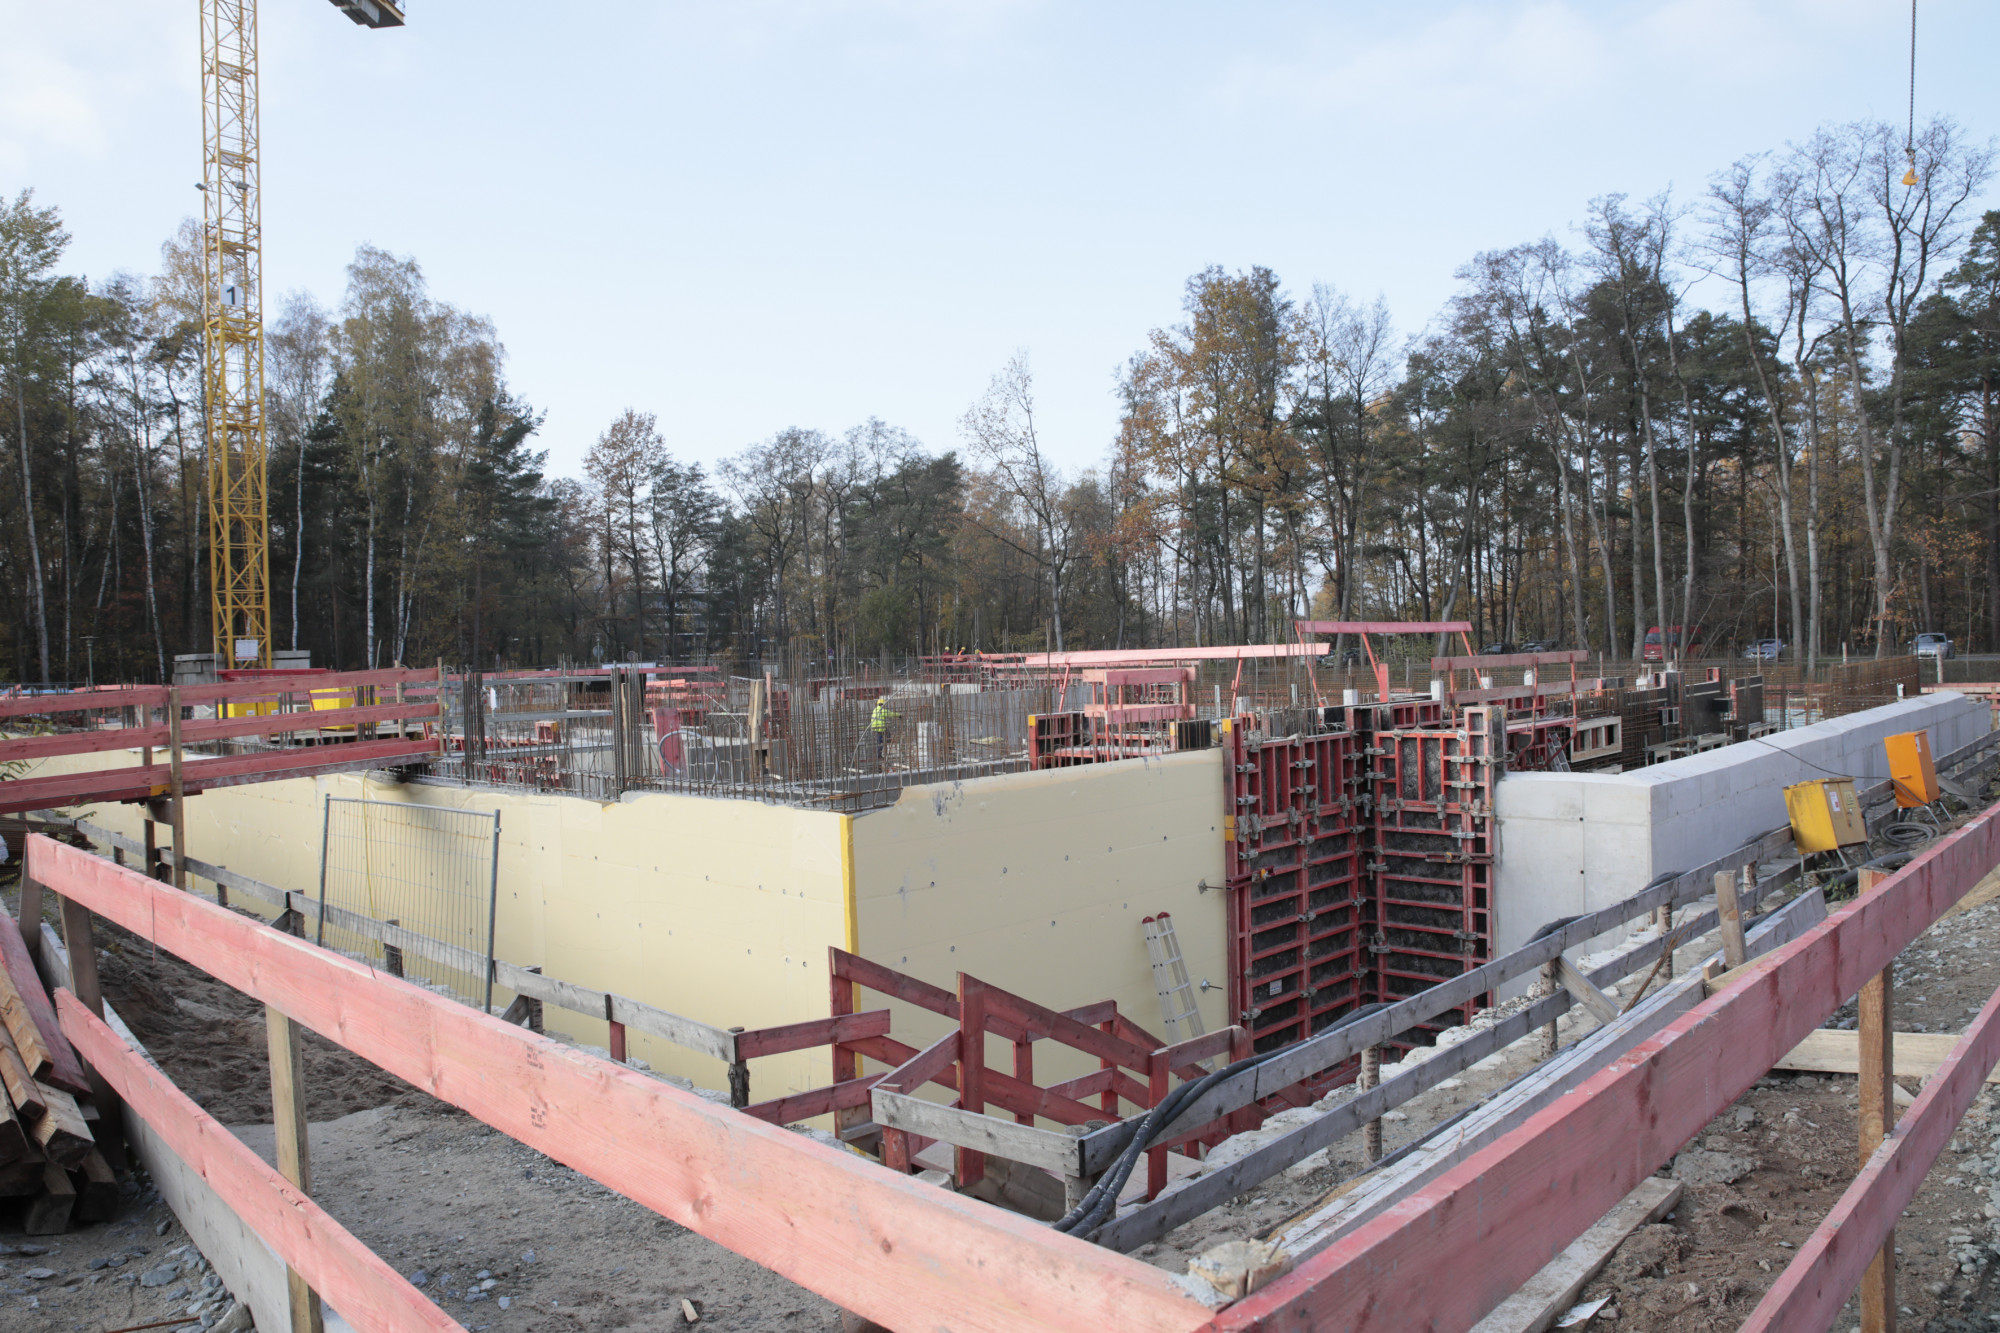
\includegraphics[width=0.9\textwidth]{imgs/ecap.jpg}
	\vfill
	{\Large\itshape following the lecture of Prof. Dr. C. van Eldik\par}
	\vfill
	{\large written by Michael Winter \par}
    \vfill
    {\large last compiled on \today}
    \vfill
	{\large summer semester 2019 + 2020\par}
	\vfill
\end{titlepage}}

\tableofcontents %Fügt ein Inhaltsverzeichnis ein
\clearpage %Beendet die Seite

\chapter*{Preface}
Before the essential contents of the lectures are presented, some remarks have to be made:\\
This script -- or rather this lecture transcript -- was written in the course of the summer semester 2019 accompanying the lecture Advanced experimental physics: Particle and astroparticle physics, read by Prof. Dr. van Eldik. In its peculiarity, this transcript is probably also incorrect and inaccurate.

\tb{If you have an overleaf account, you can mark the appropriate places in the code and leave a comment, what needs to be improved.} So others can benefit from a correction as well.

In addition, the script is constantly being revised with regard to spelling, structure and content.

\chapter{Recap particle physics}
\section{Units}
In general natural units are used: $\hbar = \mathrm c = 1$
\begin{compactitem}
    \item[$\ra$] energy, mass and momentum: $\lsb E\rsb$
    \item[$\ra$] length and time: $\lsb E\rsb ^{-1}$
    \item[$\ra$] cross section: $\lsb E\rsb ^{-2}$
\end{compactitem}
\begin{example}
\begin{align*}
    \hbar \mr c \approx \SI{200}{\mega\eV\femto\meter} \,\hat =\, 1 \longrightarrow \SI{1}{\femto \meter} \,\hat\approx\, \SI{5}{\per\giga\eV}\\
    \hbar = \SI{6.6 e-25}{\giga \eV \second} \,\hat = 1\, \longrightarrow \SI{1}{\per \giga \eV} \,\hat \approx\, \SI{6.6e-25}{\second}
\end{align*}
\end{example}
\section{Relativistic kinematics}
We will use four vector notation, i.e.
\begin{align}
    \fvec A = \lb A^0, \vec A\rb \longrightarrow A^\mu & & \text{contravariant}\\
    \lb A^0, -\vec A\rb \longrightarrow A_\mu & & \text{covariant.}
\end{align}
\paragraph{Lorentz trafos}
Remember that the Lorentz transformation $\uul \Lambda$:
\begin{align}
    A^\mu \mapsto A'^\mu = \tensor{\Lambda}{^\mu_\nu}A^\nu
\end{align}
The transformation along the $z$-axis  is a Lorentz-boost
\begin{align}
    \tensor{\Lambda}{^\mu_\nu} \ra \uul \Lambda = \mat{\gamma & 0 &  0 &- \nicefrac \gamma \beta \\ 0 & 1 & 0 & 0 \\ 0 & 0 & 1 & 0 \\ - \nicefrac \gamma \beta & 0 & 0 & \gamma} \qquad \text{ with } \beta = \frac vc, \ \gamma = \frac{1}{\sqrt{1-\beta^2}}\,.
\end{align}
The Lorentz transformation is a \tb{unitary} transformation: ''rotation in 4-space``
\paragraph{Momentum four vector}
\begin{align}
    x^\mu \ra \fvec x = \lb t, \vec x\rb, \qquad E = \gamma m \mr c^2 = \gamma m, \qquad \vec p = \gamma m \vec v = \gamma m \vec \beta
\end{align}
So it is easy to see that the momentim vector $\vec p$ is measured in units of energy. Thus we may choose the following four vector as momentum four vector (and indeed it is)
\begin{align}
    p^\mu \ra \fvec p = \lb E, \vec p \rb, \qquad \Ra E^2 = \vec p^2 +m^2\,.
\end{align}
\paragraph{Basic invariant} under Lorentz transformation is the scalar product
\begin{align}
    \fvec A \cdot \fvec B = A^\mu B_\mu = \tensor{g}{_\mu_\nu} A^\mu B^\nu = A_\mu B^\mu = A^0B^0 - \vec A \vec B\\
    \text{with } \tensor{g}{_\mu_\nu} = \tensor{g}{^\mu^\nu} = \mat{1 & 0 & 0 & 0 \\ 0 & -1 & 0 & 0 \\ 0 & 0 & -1 & 0 \\ 0 & 0 & 0 & -1} \text{ as metric tensor.} \nonumber
\end{align}
\begin{example}
    scalar product of four momentum $\fvec p$
    \begin{align}
        p^2 = p^\mu p_\mu = E^2 - \vec p^2 = m^2\,,
    \end{align}
    since $E^2 = \vec p^2 +m^2$. Therefore the (rest) mass of the particle is the same in all frames of reference.
\end{example}
\begin{example}
    total energy $\sqrt s$ of particle collision
    \begin{center}
        \begin{tikzpicture}
            \draw[very thick, -latex] (0,0) node [left] {$\fvec p_1$} -- (3,0);
            \draw[very thick, latex-] (3.5,0) -- (6.5,0) node [right] {$\fvec p_2$};
        \end{tikzpicture}
    \end{center}
    \begin{align}
        s \defi \lb \fvec p_1 + \fvec p_2\rb^2 = \lb \fvec p_1 + \fvec p_2 \rb^\mu \lb \fvec p_1 + \fvec p_2 \rb_\mu 
    \end{align}
    is Lorentz invariant since it is a scalar product. Hence it is the same in all reference frames.
\end{example}
\paragraph{Four vector derivatives}
\begin{align}
    \pa_\mu = \pdv{x^\mu} \ra \lb \pa_t, \vec \grad \rb
\end{align}
transforms like a covariant vector. Whereas
\begin{align}
    \pa^\mu = \pdv{x_\mu} \ra \qty(t, - \vec \grad)
\end{align}
transforms like a contravariant vector. The ''scalar product`` of these two is the d'Alembert operator
\begin{align}
    \Box \defi \pa_\mu\pa^\mu = \pa_t^2 - \Lap\,,
\end{align}
\begin{compactitem}
    \item[with] the Laplace operator $\Lap = \vec \grad^2$.
\end{compactitem}

\section{Elementary particles}
\paragraph{Fermions (spin $\nicefrac 12$)} Lepton sector:
\begin{align}
    \mqty(\upnu_\mr{e} \\\mr e^- ), \quad \mqty(\upnu_\upmu \\ \upmu^-),\quad \mqty(\upnu_\uptau \\ \uptau^-) \qquad \text{with charges } \mqty{Q = 0 \\ Q= -\mr e}
\end{align}
They come with a certain mass hierarchy $m_\mr{e} < m_\upmu < m_\uptau$ and the assumption in the standard model that $m_\upnu = 0$ regardless of the neutrino flavour. However we know $m_\upnu >0$ but very small.

Quark sector:
\begin{align}
    \mqty(u \\ d), \quad \mqty(c \\ s), \quad \mqty( t \\ b) \qquad \text{with charges } \mqty{Q = \frac 23 \mr e \\ Q = - \frac 13 \mr e}
\end{align}
Free particles are bounded states with $qq'q''$ as baryons and $q\bar q$ as mesons. Additionally, only colour-neutral particle states are observed.

Both sectors come with the respective 6 anti-particles.

\paragraph{Bosons (spin $1$)} exchange particles of interactions
\begin{compactitem}
    \item[$\upgamma$:] em. interaction, $m=0$, $Q=0$ couples to electric charge
    \item[$Z^0$:] weak interaction, $m = \SI{91}{\giga\eV}$, $Q=0$, couples to weak charge
    \item[$W^\pm$:] weak interaction, $m = \SI{80}{\giga\eV}$, $Q = \pm \mr e$, couples to weak charge
    \item[$g$:] strong interaction, $m=0$, $Q=0$\\
    8 gluons in total, carry colour charge\\
    couple to quarks and to one another (''self-coupling``)
\end{compactitem}

\paragraph{Scalar (spin $0$)}
\begin{compactitem}
    \item[$H^0$:] Higgs boson, brings mass to $Z^0$, $W^\pm$ (''spontaneous symmetry breaking``)\\
    $m = \SI{125}{\giga\eV}$
\end{compactitem}

\section{Feynman diagrams}
These give pictorial representations of particle reactions. Perturbative expansion of scattering ''in a potential`` into leading order and higher order terms, if necessary.
\begin{example}
    electromagnetic scattering (leading order)
    \begin{multicols}{2}
        \begin{center}
            \begin{tikzpicture}
                \begin{feynman}
                \vertex (a1);
                \vertex [below right = 2cm of a1] (b1);
                \vertex [above right = 2cm of b1] (a2);
                \vertex [below = 2cm of b1] (c1);
                \vertex [below left = 2cm of c1] (d1);
                \vertex [below right = 2cm of c1] (d2);
                \vertex [below left = 0.5cm of d1] (z1);
                \vertex [right = 1.6cm of z1] (z2);
                \vertex [below right = 0.5cm of d2] (z4);
                \vertex [left = 1.6cm of z4] (z3);
                \vertex [below = 2.2cm of c1] (y1) {particles};
                \diagram*{
                (a1) -- [fermion, edge label = $\mr e^-$, momentum' = $\fvec p_1$] (b1) -- [fermion, edge label = $\mr e^-$, momentum' = $\fvec p_1'$] (a2),
                (b1) -- [photon, edge label' = $\upgamma$, momentum = $\fvec q$] (c1),
                (d1) -- [fermion, edge label' = $\upmu^-$, momentum = $\fvec p_2$] (c1) -- [fermion, edge label' = $\upmu^-$, momentum = $\fvec p_2'$] (d2);
                };
                \draw[decoration={brace}, decorate] (z2.south) -- node[below] {incoming} (z1.south west);
                \draw[decoration={brace}, decorate] (z4.south east) -- node[below] {outgoing} (z3.south);
                \end{feynman}
            \end{tikzpicture}
        \end{center}
        \begin{compactitem}
            \item[with] $\fvec q$: 4-momentum transfer
        \end{compactitem}
        We will describe this in $\fvec q^2$ (which is Lorentz invariant)
        \begin{align}
            \fvec q^2 = \qty(\fvec p_1 - \fvec p_1')^2 \neq 0
        \end{align}
        The inequity to zero means that it is off mass-shell\\
        $\Ra$ virtual particle because it carries to much/less energy
    \end{multicols}
    
    Next question to ask is: What is the \tb{transition amplitude}?
    \begin{multicols}{2}
        \begin{center}
            \begin{tikzpicture}
                \begin{feynman}
                    \vertex (b1);
                    \vertex [above left  = 1cm of b1] (a1) {$\mr e^-$};
                    \vertex [above right = 1cm of b1] (a2) {$\mr e^-$};
                    \vertex [below = 1cm of b1] (c1);
                    \vertex [below left  = 1cm of c1] (d1) {$\upmu^-$};
                    \vertex [below right = 1cm of c1] (d2) {$\upmu^-$};
                    \diagram*{
                        (a1) -- [fermion] (b1) -- [fermion] (a2),
                        (b1) -- [scalar, momentum = {$\fvec q, M$}] (c1),
                        (d1) -- [fermion] (c1) -- [fermion] (d2);
                    };
                \end{feynman}
            \end{tikzpicture}
        \end{center}
    \begin{align}
        amplitude \propto g_1 \frac{1}{\fvec q^2 - M^2} g_2
    \end{align}
    \begin{compactitem}
        \item[with] $g_{1,2}$: coupling strength between fermion and exchange particle
        \item[] $\nicefrac{1}{\fvec q^2-M^2}$: boson propagator for exchange particle of mass $M$
    \end{compactitem}
    \end{multicols}
    Here the electromagnetic and the weak interaction contribute, i.e.
    \begin{align*}
        \feynmandiagram[vertical= b to d, baseline = -2cm]{
        a [particle = $\mr e^-$] -- [fermion] b -- [fermion] c [particle = $\mr e^-$],
        b -- [photon, edge label = $\upgamma$] d,
        e [particle = $\upmu^-$]-- [anti fermion] d -- [anti fermion] f [particle = $\upmu^-$],
        };
        + 
        \feynmandiagram[vertical= b to d, baseline = -2cm]{
        a [particle = $\mr e^-$] -- [fermion] b -- [fermion] c [particle = $\mr e^-$],
        b -- [scalar, edge label = $Z^0$] d,
        e [particle = $\upmu^-$]-- [anti fermion] d -- [anti fermion] f [particle = $\upmu^-$],
        };
        = e \frac{1}{\fvec q^2}e + g_1 \frac{1}{\fvec q^2 - M_Z^2} g_2
    \end{align*}
    Last question: What is the \tb{cross section}?\\
    It is proportional to the transition probability
    \begin{align}
        \sigma \propto W, \qquad W \propto \qty| amplitude_1 + amplitude_2 |^2 \propto \frac{\mr e^4}{\fvec q^4}
    \end{align}
    The factor $\nicefrac{1}{\fvec q^4}$ leads to a rapid decrease of the cross section as momentum transfer increases.
    \begin{center}
        \begin{tikzpicture}
            \draw[-latex] (-3.25,0) node [left] {$\fvec p_1$} -- (-.25,0);
            \draw[latex-] (.25,0) -- (3.25,0) node [right] {$\fvec p_2$};
            \draw[-latex] (0,0,0) -- (3,1.5,0);
            \coordinate (O) at (0,0,0);
            \tdplotsetcoord{P1}{3.5}{90}{30};
            \tdplotsetcoord{P2}{3.5}{90}{20};
            \tdplotsetcoord{P3}{3.5}{30}{30};
            \tdplotsetcoord{P4}{3.5}{0}{30};
            \draw[-latex] (P1) -- (P2);% -- (P3) -- (P4) -- (P1);
            \draw[dashed] (3.5,90,30) arc (30:20:3.5);
        \end{tikzpicture}
    \end{center}
\end{example}
\chapter{Covariant description of relativistic particles}
\section{Non-relativistic quantum mechanics}
Recall the energy-momentum relation
\begin{align}
    E = \frac{1}{2m} \qty|\vec p|^2\,.
\end{align}
By identifying $E \ra \ti \hbar \pa_t$, $\vec p \ra -\ti \hbar \vec \grad$, we get an operator equation, i.e. the Schrödinger equation
\begin{align}\label{eq:schroedinger}
    \boxed{\qty(\ti \pa_t + \vec \grad ^2 \frac{1}{2m}) \phi \qty(\vec x, t) = 0}
\end{align}
\begin{compactitem}
    \item[with] $\phi \qty(\vec x, t) \in \mb C$ as the one-particle wave function.
\end{compactitem}
We can get the statistical interpretation via $\qty | \phi | \dd[3]{x}$ $\hat =$ probability to find particle in volume $\dd[3]{x}$ at time $t$ and we can obtain the localisation probability density
\begin{align}
    \ra \quad \rho = \rho \qty (\vec x, t) \defi \qty|\phi \qty(\vec x, t)|^2\,.
\end{align}
\begin{multicols}{2}
    \begin{center}
        \begin{tikzpicture}
            \draw (0.,-0.05) to [curve through = {(1.,0.) .. (1.2,0.8) .. (0.4,1.6) .. (0.,2.) .. (-0.5,0.75)}] (0.,-0.05);
            \foreach \i in {-0.2,0.2,0.6}
                \draw[-latex] (\i,1.2-\i) to [curve through = {(\i+0.2,1.8-\i)}] (\i+0.1,2.4);
            \foreach \i in {-0.2,-0.5,-0.8}
                \draw[-latex] (\i,-1.4-\i) to [curve through = {(\i-0.2,-0.6-\i)}] (\i,-0.2-\i);
            \node at (1.,2.6) {$\vec j$};
            \node at (0,0.5) {$\rho$};
            \node at (1.4,0) {$\dd[3]{x}$};
        \end{tikzpicture}
    \end{center}
    From electrodynamics we get the continuity equation:
    \begin{align}\label{eq:continuity}
        \boxed{\pa_t \rho + \vec \grad \vec j = 0}
    \end{align}
    \begin{compactitem}
        \item[with] $\vec j \qty(\vec x, t)$ as the \tb{probability density current}.
    \end{compactitem}
\end{multicols}
How does $\vec j$ depend on the wave function $\phi$?
\begin{align*}
    \qty(-\ti \phi^*) \cdot (\cref{eq:schroedinger}) & = \phi^*\pa_t \phi - \frac{\ti}{2m} \phi^* \vec \grad ^2 \phi = 0 \\
    \qty(- \ti \phi) \cdot (\cref{eq:schroedinger})^* & = - \phi \pa_t \phi^* - \frac{\ti}{2m} \phi \vec \grad ^2 \phi^* = 0
\end{align*}
By subtracting these two equations we get
\begin{align}
    \Ra \quad \underbrace{\qty(\phi^*\pa_t \phi + \phi \pa_t \phi^*)}_{\pa_t \qty(\phi^*\phi) = \pa_t \qty|\phi|^2} - \frac{\ti}{2m} \underbrace{\qty(\phi^* \vec \grad ^2 \phi - \phi \vec \grad^2 \phi^*)}_{\vec \grad \qty(\phi^*\vec \grad \phi - \phi \vec \grad \phi^*)} = 0
\end{align}
and by using the continuity \cref{eq:continuity} we get an explicit expression for the probability density current
\begin{align}
    \boxed{ \vec j = - \frac{\ti}{2m}\qty(\phi^*\vec \grad \phi - \phi \vec \grad \phi^*) }\,.
\end{align}
The probability density current, based on the Schrödinger equation, is not covariant. This means that the Schrödinger equation treats time and space different.

\section{Relativistic particles: Klein-Gordon equation}
Now we use the \tb{relativistic} energy-momentum relation
\begin{align}
    E^2 = \vec p^2 +m^2 \qquad E \ra \ti \hbar \pa_t, \quad \vec p \ra \ti \hbar \vec \grad\nonumber \\
    \Ra \quad \boxed{\qty(\pa_t^2 - \Lap +m^2) \phi \qty(\vec x, t) = 0}\,. \label{eq:KGe}
\end{align}
This is the so-called \tb{Klein-Gordon equation}. By using four vector notation
\begin{align}
    p^\mu \ra \mqty(E \\ \vec p) \ra \mqty(\ti \pa_t \\ - \ti \vec \grad) \ra \ti \pa^\mu \quad \Ra \quad \boxed{\qty(\pa_\mu\pa^\mu + m^2) \phi = 0}\,,
\end{align}
which denotes the Klein-Gordon equation in covariant form. Since the scalar product and the mass are Lorentz invariant, this KG equation is too.\\
$\ra$ Klein-Gordon equation describes spin-0 particles.

The continuity equation thus is
\begin{align}
    \pa_t \rho + \vec \grad \vec j = 0 \quad \ra \quad \boxed{\pa_\mu j^\mu = 0}\,.
\end{align}
How do $\rho$ and $\vec j$ depend on $\phi$?
\begin{align}\label{eq:four_density_KGe}
    \rho = \ti \qty(\phi^*\pa_t \phi - \phi \pa_t \phi^*), \quad \vec j = - \ti \qty(\phi^* \vec\grad \phi - \phi  \vec \grad \phi^*)
\end{align}
and the for vector current is
\begin{align}
    \boxed{j^\mu = \ti \qty(\phi^* \pa^\mu \phi - \phi\pa^\mu \phi^*)}\,.
\end{align}
The fundamental free-particle solution for the KGe is given by
\begin{align}\begin{split}
    \phi \qty(\vec x,t) \equiv \phi (\fvec x) & = N \cdot \exp(\ti \qty(\vec p\vec x - Et))\\
    & = N \exp(- \ti p_\mu x^\mu) = N \exp(-\ti \fvec p\fvec x)
\end{split}\end{align}
\begin{compactitem}
    \item[with] $N$ as the normalisation.
\end{compactitem}
By inserting this into the probability density current (\cref{eq:four_density_KGe}), we get
\begin{align}
    \boxed{j^\mu = 2 p^\mu \qty|N|^2}
\end{align}
for free particles. Note that espacially $\rho = 2 E \qty|N|^2$.
\begin{itemize}[$\ra$]
    \item Localisation probability $\rho \dd[3]{x}$, but under Lorentz boost $\dd[3]{x} \ra \frac 1\gamma \dd[3]{x}$, since $\rho \propto E \propto \gamma$. This effect is compensated for the probability density current $\vec j \propto \vec p$.
    \item Particle current $\vec j$ in the direction of the particle momentum $\vec p$.
\end{itemize}
What are the eigenvalues of the free-particle solution?
\begin{align}
    &\qty(\pa_\mu \pa^\mu + m^2) \exp(-\ti \fvec p\fvec x) = 0 \nonumber \\
    &\Ra\quad \qty(\qty(-\ti)^2 p_\mu p^\mu + m^2) \exp(-\ti \fvec p \fvec x) = 0 \nonumber \\
    &\Ra\quad - p_\mu p^\mu + m^2 = 0, \quad p_\mu p^\mu = m^2 = E^2 - \vec p^2 \nonumber \\
    &\Ra\quad \boxed{E = \pm \sqrt{\vec p^2 + m^2}}
\end{align}
So we get two solutions for the particle energy. However, the negative solution $E < 0 \Ra \rho < 0$ is unphysical! There is one way out, the Feynman-Stückelberg approach. Here we interpret $\rho$ as a charge density.
\begin{itemize}
    \item[$\ra$] Can be negative, since particles can have negative charge.
    \item[$\ra$] Interpret $j^\mu$ as charge current.
    \item[$\Ra$] $j^\mu \ra j'^\mu = Q j^\mu$ with $Q$ as particle charge.
\end{itemize}

\begin{example}
    electron, $ Q= -\mr e$
    
    By assuming an electron with spin 0, we get
    \begin{align}
        j^\mu \qty(\mr e^-) = - \ti \mr e \qty(\phi^* \pa^\mu \phi - \phi \pa^\mu \phi^*)\,.
    \end{align}
    Free particle solution ($E>0$):
    \begin{align}
        j^\mu \qty(\mr e^-) = -2 \mr e p^\mu \qty|N|^2 \ra - 2 \mr e \qty|N|^2 \mqty(E \\ \vec p)
    \end{align}
    For $E<0$: Consider anti muon with $E>0$
    \begin{align}
        \fvec j \qty(\mu^+) = 2 \mr e \fvec p \qty|N|^2 = 2 \mr e \qty|N|^2 \mqty(E \\ \vec p) = - 2 \mr e \qty|N|^2 \mqty(-E \\ -\vec p)  = - \fvec j \qty(\mu^-)\,.
    \end{align}
    So we get a muon with $E<0$, that moves backwards.
\end{example}
\begin{itemize}
    \item[$\ra$] solution with $E<0$ can be used to describe antiparticles with $E' = -E$
\end{itemize}
\begin{align*}
    \begin{tikzpicture}
        \begin{feynman}
        \vertex (a1) {$\mr e^-$};
        \vertex [below right = 2.5cm of a1] (b1);
        \vertex [above right = 2cm of b1] (a2) {$\mr e^-$};
        \vertex [below = 2cm of b1] (c1);
        \vertex [below left = 2cm of c1] (d1) {$\upmu^+$};
        \vertex [below right = 2cm of c1] (d2) {$\upmu^+$};
        \vertex [right = 1cm of d1] (j1);
        \vertex [left = 1cm of d2] (j2);
        \vertex [right = 1cm of a1] (i1);
        \vertex [left = 1cm of a2] (i2);
        \vertex [below = 1cm of b1] (b2);
        \vertex [right = 2.5cm of b2] (e) {$\hat =$};
        \diagram*{
        (a1) -- [fermion, momentum' = $\fvec p_A$] (b1) -- [fermion, momentum' = $\fvec p_C$] (a2);
        (b1) -- [photon, edge label' = $\upgamma$] (c1);
        (d1) -- [anti fermion, momentum = $\fvec p_B$] (c1) -- [anti fermion, momentum = $\fvec p_D$] (d2);
        (j1) -- [draw = none, half left, momentum = $\ $, edge label' = $j^\mu \qty(\upmu^+)$] (j2);
        (i1) -- [draw = none, half right, momentum' = $\ $, edge label = $j^\mu \qty(\mr e^-)$] (i2);
        };
        \vertex [right = 6cm of a1] (z1) {$\mr e^-$};
        \vertex [below right = 2.5cm of z1] (y1);
        \vertex [above right = 2cm of y1] (z2) {$\mr e^-$};
        \vertex [below = 2cm of y1] (x1);
        \vertex [below left = 2cm of x1] (w1) {$\upmu^-$};
        \vertex [below right = 2cm of x1] (w2) {$\upmu^-$};
        \vertex [right = 1cm of w1] (k1);
        \vertex [left = 1cm of w2] (k2);
        \vertex [right = 1cm of z1] (l1);
        \vertex [left = 1cm of z2] (l2);
        \diagram*{
        (z1) -- [fermion, momentum' = $\fvec p_A$] (y1) -- [fermion, momentum' = $\fvec p_C$] (z2);
        (y1) -- [photon, edge label' = $\upgamma$] (x1);
        (w1) -- [fermion, rmomentum = $-\fvec p_B$] (x1) -- [fermion, rmomentum = $-\fvec p_D$] (w2);
        (k2) -- [draw = none, half right, momentum' = $\ $, edge label = $j^\mu \qty(\upmu^-)$] (k1);
        (l1) -- [draw = none, half right, momentum' = $\ $, edge label = $j^\mu \qty(\mr e^-)$] (l2);
        };
        \end{feynman}
    \end{tikzpicture}
\end{align*}
Consequence: Can use particle states with $p^\mu \ra - p^\mu$ for description of antiparticles.

\section{Crossing symmetry}
The description of scattering processes is highly symmetric under the exchange of space and time: This originates in the fact that wave equations treat time and space the same way.
\begin{example}
    $\mr e^- \upmu^-$ scattering in QED
    
    By exchange of time and space, the Feynman diagram changes as:
    \begin{center}
        \begin{tikzpicture}
            \begin{feynman}
                \vertex (a1) {$\mr e^-$};
                \vertex [below right = 2.5cm of a1] (b1);
                \vertex [above right = 2cm of b1] (a2) {$\mr e^-$};
                \vertex [below = 2cm of b1] (c1);
                \vertex [below left = 2cm of c1] (d1) {$\upmu^+$};
                \vertex [below right = 2cm of c1] (d2) {$\upmu^+$};
                \vertex [right = 1cm of d1] (j1);
                \vertex [left = 1cm of d2] (j2);
                \vertex [right = 1cm of a1] (i1);
                \vertex [left = 1cm of a2] (i2);
                \vertex [below = 1cm of b1] (b2);
                \vertex [right = 3cm of b2] (e) {$\hat =$};
                \diagram*{
                (a1) -- [fermion] (b1) -- [fermion] (a2);
                (b1) -- [photon, edge label' = $\upgamma$] (c1);
                (d1) -- [anti fermion] (c1) -- [anti fermion] (d2);
                (j1) -- [draw = none, half left, momentum = $\ $, edge label' = $j^\mu \qty(\upmu^+)$] (j2);
                (i1) -- [draw = none, half right, momentum' = $\ $, edge label = $j^\mu \qty(\mr e^-)$] (i2);
                };
                \vertex [right = 3cm of e] (y1);
                \vertex [below left = 2cm of y1] (z1) {$\mr e^-$};
                \vertex [above left = 2cm of y1] (z2) {$\mr e^+$};
                \vertex [right = 2cm of y1] (x1);
                \vertex [above right = 2cm of x1] (w1) {$\upmu^-$};
                \vertex [below right = 2cm of x1] (w2) {$\upmu^+$};
                \vertex [below = 1cm of w1] (k1);
                \vertex [above = 1cm of w2] (k2);
                \vertex [above = 1cm of z1] (l1);
                \vertex [below = 1cm of z2] (l2);
                \diagram*{
                (z1) -- [fermion] (y1) -- [fermion] (z2);
                (y1) -- [photon, edge label' = $\upgamma$] (x1);
                (w1) -- [anti fermion] (x1) -- [anti fermion] (w2);
                (k2) -- [draw = none, half left, momentum = $\ $, edge label' = $j^\mu \qty(\upmu^-)$] (k1);
                (l1) -- [draw = none, half right, momentum' = $\ $, edge label = $j^\mu \qty(\mr e^-)$] (l2);
                };
            \end{feynman}
        \end{tikzpicture}
    \end{center}
    This is equivalent to a counter clockwise rotation by \SI{90}{\degree}. The resulting diagram represents $\mr e^+ \mr e^-$ annihilation followed by $\mu^+\mu^-$ creation.
\end{example}
By exchanging the incoming anti muon by an outgoing muon in the $\upmu^+\upmu^-$ annihilation, we get the diagram:
\begin{center}
    \begin{tikzpicture}
        \begin{feynman}
        \vertex (y1);
        \vertex [below = 1.8cm of y1] (s);
        \vertex [right = 0.7cm of s] (z1) {$\upmu^-$};
        \vertex [above left = 2cm of y1] (z2) {$\upmu^-$};
        \vertex [right = 2cm of y1] (x1);
        \vertex [above right = 2cm of x1] (w1) {$\mr e^-$};
        \vertex [below right = 2cm of x1] (w2) {$\mr e^+$};
        \diagram*{
        (z1) -- [anti fermion] (y1) -- [anti fermion] (z2);
        (y1) -- [photon, edge label' = $\upgamma$] (x1);
        (w1) -- [anti fermion] (x1) -- [anti fermion] (w2);
        };
        \end{feynman}
    \end{tikzpicture}
\end{center}
This is $\upmu^-$-Bremsstrahlung with subsequent pair creation.

All these processes share the same common transition amplitude, as they contain the same basic interaction. The only difference lies in the momenta of external particles.\\
$\ra$ Thus it is much easier to calculate the related processes once the transition amplitude of one process is known.

\paragraph{Mandelstam variables}
Assume any process $AB \ra CD$ with the Feynman diagram:
\begin{center}
    \begin{tikzpicture}
        \begin{feynman}
            \vertex (b1);
            \vertex [above left = 1cm of b1] (a1) {$\fvec p_A$};
            \vertex [above right = 1cm of b1] (a2) {$\fvec p_C$};
            \vertex [below = 1cm of b1] (c1);
            \vertex [below left = 1cm of c1] (d1) {$\fvec p_B$};
            \vertex [below right = 1cm of c1] (d2) {$\fvec p_D$};
            \vertex [below = 0.75cm of b1] (m);
            \vertex [left = 1.5cm of m] (s);
            \diagram*{
            (a1) -- [fermion] (b1) -- [fermion] (a2);
            (b1) -- [photon] (c1);
            (d1) -- [fermion] (c1) -- [fermion] (d2);
            (s) -- [draw = none, momentum = {[arrow style = myblue] $s$}] (m);
            (a2) -- [draw = none, momentum = {[arrow style = myblue] $t$}] (d2);
            };
        \end{feynman}
    \end{tikzpicture}
\end{center}
Here we define the Mandelstam variables
\begin{align}
    s \defi \qty(\fvec p_A + \fvec p_B)^2, \qquad t \defi \qty(\fvec p_A - \fvec p_C)^2, \qquad u \defi \qty(\fvec p_A - \fvec p_D)
\end{align}
with the identity
\begin{align}
    s + t + u = m_A^2 + m_B^2 + m_C^2 + m_D^2\,.
\end{align}
A crossing of processes therefore generally means interchanging the Mandelstam variables.

\section{Interaction of a particle in a potential}\label{sec:Interaction_particle_potential}
We will now alternate the free Hamiltonian $H_0$ with a potential, i.e.
\begin{align}
    H_0 \ra H_0 + V\qty(\fvec x)\,.
\end{align}
The potential $V$ allows for the transformation from initial to final state $\phi_\mr{i} \ra \phi_\mr{f}$. We can calculate the transition amplitude:
\begin{align}
    T_\mr{fi} = \braket{\phi_\mr{f} | V | \phi_\mr{i}} + \text{higher orders}
\end{align}
Assumption: $V$ is small and only present for a short time $T$
\begin{itemize}[$\ra$]
    \item $\phi_\mr{i}$, $\phi_\mr{f}$ can be treated as plane waves with energy $E_\mr{i}$, $E_\mr{f}$
    \item $T_\mr{fi}$ can be extended in a perturbation series
\end{itemize}
We will do this as ''Born approximation``
\begin{align}
    T_\mr{fi} \approx \braket{\phi_\mr{f}| V | \phi_\mr{i}} = - \ti \int \phi_\mr{f}^* \qty(\fvec x) V\qty(\fvec x) \phi_\mr{i} \qty(\fvec x) \dd[4]x\,.
\end{align}
\begin{center}
    \begin{tikzpicture}
        \begin{feynman}
            \vertex (b1);
            \vertex [above left = 1cm of b1] (a1) {$\phi_\mr{i}$};
            \vertex [above right = 1cm of b1] (a2) {$\phi_\mr{f}$};
            \vertex [below = 1cm of b1] (c1) {$V\qty(\fvec x)$};
            \diagram*{
            (a1) -- [fermion] (b1) -- [fermion] (a2);
            (b1) -- [photon] (c1);
            };
        \end{feynman}
    \end{tikzpicture}
\end{center}
Further assumption: $V\qty(\fvec x)$ does not depend on time.
\begin{align}\begin{split}
    T_\mr{fi} & = \underbrace{-\ti \int \phi_\mr{f}^* \qty(\vec x) V\qty(\vec x) \phi_\mr{i}\qty(\vec x) \dd[3]{x}}_{V_\mr{fi}} \cdot \int\limits_{-\nicefrac T2}^{\nicefrac T2} \underbrace{\exp(-\ti \qty(E_\mr{f} - E_\mr{i})t) \dd{t}}_{\substack{\text{two components of}\\ \text{free-particle wave function}}} \\
    & = -\ti V_\mr{fi} 2 \pi \delta \qty(E_\mr{f} - E_\mr{i})
\end{split}\end{align}
The transition rate (probability per unit of time) then reads
\begin{align}
    W_\mr{fi} = \gamma_\mr{fi} = 2 \pi \qty|V_\mr{fi}|^2 \delta \qty(E_\mr{f} - E_\mr{i})\,.
\end{align}
For many possible final states $\phi_\mr{f}$ integrated over in the measurement, we will sum/integrate over them
\begin{align}\begin{split}
    W_\mr{fi} & = 2\pi \int_0^{E_\mr{f}} \rho_\mr{f} \qty(E_\mr{f}) \qty|V_\mr{fi}|^2 \delta @ty(E_\mr{f} - E_\mr{i}) \dd{E_\mr{f}}\\
    \Ra\quad \boxed{ W_\mr{fi} = 2\pi \qty|V_\mr{fi}|^2 \rho_\mr{f} \qty(E_\mr{i})}
\end{split}\end{align}
\begin{compactitem}
    \item[with] $\rho_\mr{f}$: the phase space density.
\end{compactitem}
The boxed equation above is called \tb{Fermi's Golden Rule}.



\chapter{Experimentelle Aspekte\label{chap:3}}
\begin{compactitem}
\item Messgröße für Vergleich Experiment - Theorie
\item Durchgang von Teilchen durch Materie\\
$\ra$ Teilchennachweis
\item Biologische Strahlenwirkung\\
$\ra$ Dosimetrie
\end{compactitem}
\section{Wirkungsquerschnitt und Lebensdauer}
\tb{Wirkungsquerschnitt (WQ)}\\
= \glqq effektive Trefferfläche\grqq{} für Reaktion zweier Teilchen

\begin{figure}[!ht]
\centering
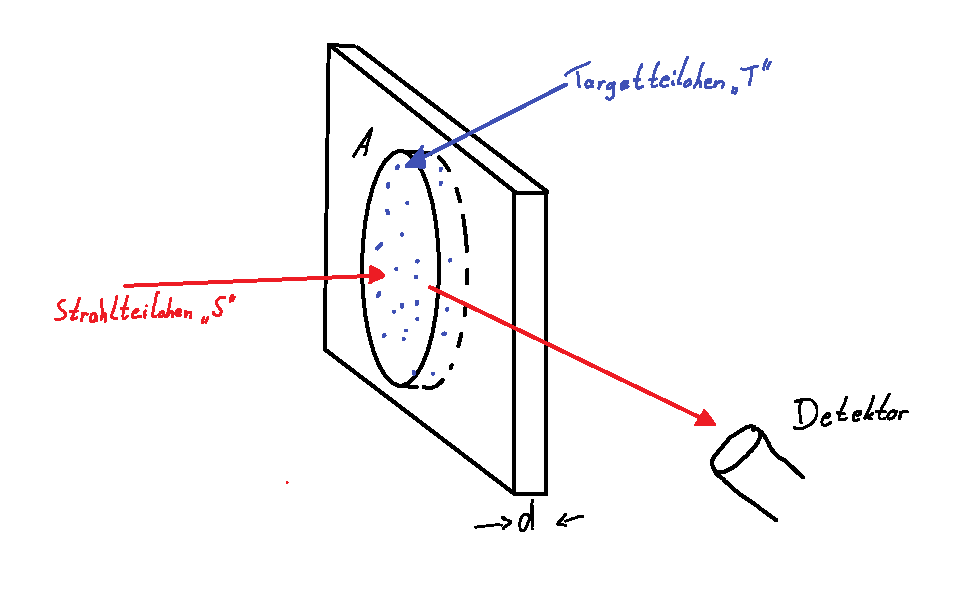
\includegraphics[width=.5\textwidth]{imgs/ep5-fig-3-1.pdf}
\caption{Bestrahlung eines Streuobjektes und anschließender Detektion der gestreuten Teilchen}
\end{figure}
Strahlteilchen streuen an dem Volumen $A\cdot d$ ($A$: Streufläche, $d$: Streudicke). Beschreibe Strahlteilchen durch Stromdichte $j_S= \frac{\Delta N_S}{A\Delta t}$ und Targetteilchen durch Dichte $\rho_T =\frac{N_T}{V}= \frac{N_T}{Ad}$. Die Zahl der Reaktionen ist dann
\begin{align}
\boxed{\frac{\Delta N_{WW}}{\Delta t} = \frac{\Delta N_S}{\Delta t}N_T \cdot \underbrace{\frac{\sigma_{ST}}{A}}}\\
\text{\footnotesize WW-Wskt. pro WW-Versuch} \nonumber
\end{align}
$\Delta N_S \cdot N_T $ = Zahl der WW-Versuche.\\
$\sigma_{ST} = $ WQ für $S$-$T$-WW und hängt von der Art der Teilchen $S$, $T$ sowie von $E_\mr{CMS}$ ab, $\left[\sigma_{ST}\right] = \mr{m^2}$. Mit $\dot{N}_{WW}$ als WW-Rate lässt sich schreiben
\begin{align}
\Ra \boxed{ \sigma_{ST} = \frac{\dot{N}_{WW}}{j_S\cdot N_T} }
\end{align}
\begin{figure}[!ht]
\captionsetup{type=figure}
\centering
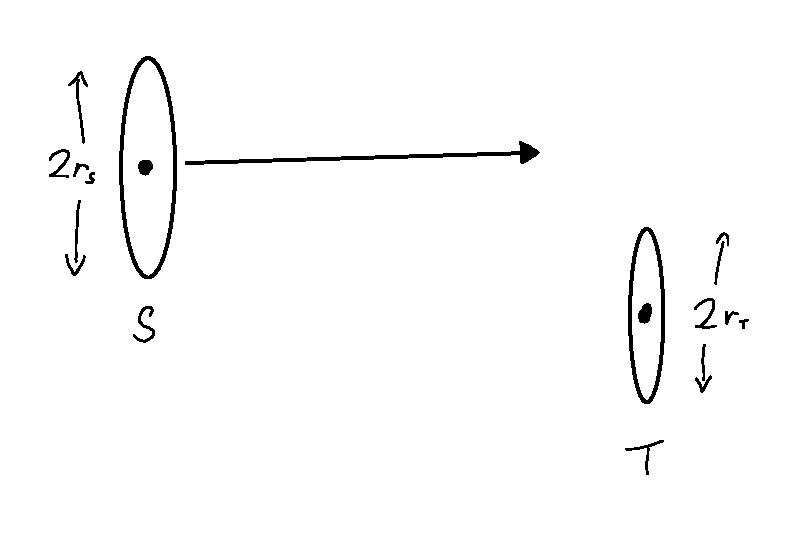
\includegraphics[width=.5\textwidth]{imgs/ep5-fig-3-2.pdf}
\caption{Geometrische Interpretation des WQ}
\end{figure}
Durch eine geometrische Interpretation des WQ (zwei Kugeln stoßen), würde man klassisch erhalten:
\begin{align}
\Ra \sigma_{ST}^{geo}= \pi \left( r_S + r_T\right)^2
\end{align}
Dies gilt jedoch \tb{nur} für ausgedehnte Objekte, aber nicht für Elementarteilchen.
\begin{framed}
\tb{Einheit von $\sigma$}: $1\,\mr{barn}=1\,\mr b = 10^{-28}\,\mr{m^2}$
\end{framed}
\begin{itemize}
\item Beispiel 1: $p+p \ra X$
\begin{align}
\begin{split}
r_p = 10^{-15}\,\mr{m}\\
\Ra \sigma_{pp}^{geo} = 4\pi r_p^2 = 1.2 \cdot 10^{-29}\,\mr{m^2} = 120\,\mr{mb}
\end{split}
\end{align}
Gemessen: $\sigma_{pp}^{exp}$ ist energieabhängig und kleiner
\begin{align*}
\sigma^{tot} = \sigma^{el} + \sigma^{Coul}
\end{align*}
\begin{center}
\captionsetup{type=figure}
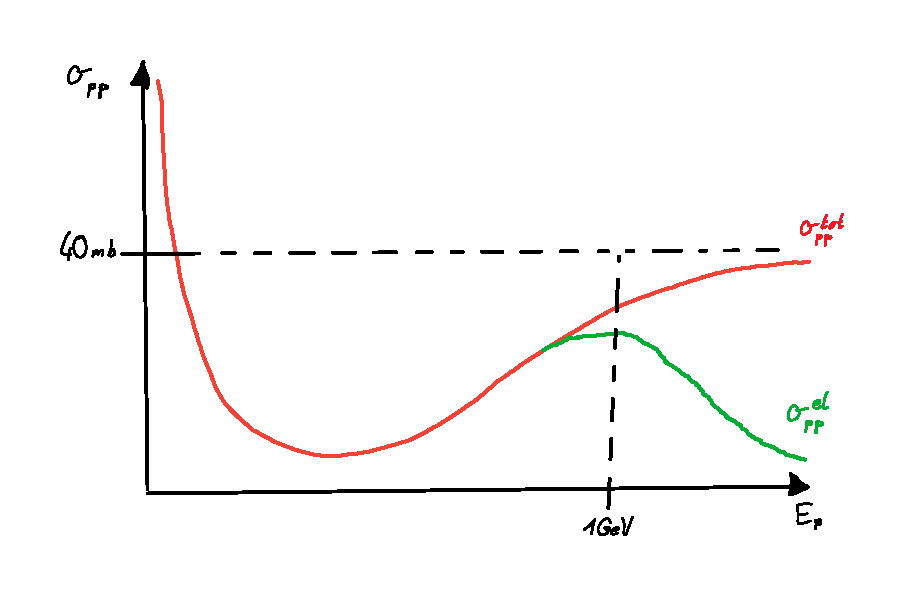
\includegraphics[width=.5\textwidth]{imgs/ep5-fig-3-3.pdf}
\captionof{figure}{Abhängigkeit des WQ von der Energie (hier für $pp$-WW)}
\end{center}

\item Beipiel 2: $\nu+p \ra X$\\
Wenn $r_\nu = 0 \Ra \sigma_{\nu p}^{geo} = 30$\,mb. Gemessen:
\begin{align}
\boxed{\sigma_{\nu p}^{exp} = 0.7\cdot 10^{-42}\,\mr{m^2}}
\end{align}
$\lt$ Faktor $\sim 10^{-13}$!
\item[$\Ra$] WQ in Teilchenphysik ist i.A. \tb{nicht} durch Geometrie der Teilchen gegeben
\item[$\Ra$] WQ ist \tb{stark} energieabhängig
\end{itemize}

 \tb{Differentieller WQ}\\
Effektive Trefferfläche für den Endzustand in einem bestimmten kinematischen Intervall, z.B. Raumwinkel.
\begin{figure}[!ht]
\centering
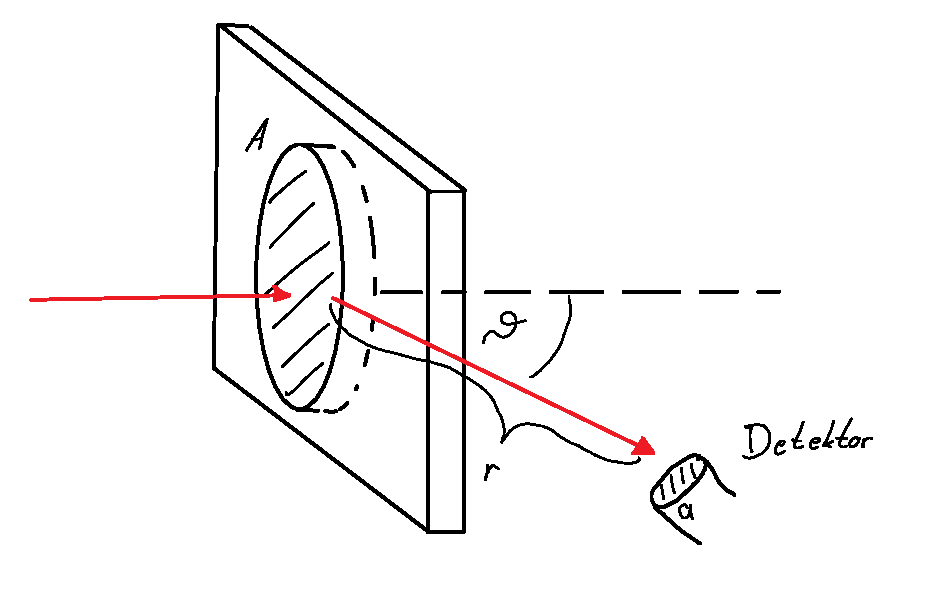
\includegraphics[width=.5\textwidth]{imgs/ep5-fig-3-4.pdf}
\caption{Skizze zur Raumwinkeldetektion}
\end{figure}

  Es gilt hier:
\begin{align}
\begin{split}
\Delta \Omega = \frac{a}{r^2}\\
\Ra \frac{\Delta N_{WW}}{\Delta t} = \frac{N_S}{\Delta t} \cdot N_T \cdot \frac{\Delta \sigma_{ST}^{\Delta \Omega}}{A}\\
\boxed{ \Delta \sigma = \frac{\Pa \sigma_{ST}}{\Pa \Omega}\cdot \Delta \Omega }
\end{split}
\end{align}
Der differentielle WQ ist also:
\begin{align}
\frac{\Pa \sigma_{ST}}{\Pa \Omega} = \underbrace{\frac{\Delta N_{WW}}{\Delta \Omega}}_\text{Messgröße} \cdot \underbrace{\frac{A}{N_S N_T}}_\text{Aufbau}
\end{align}
\begin{framed}
\tb{Anmerkung:}\\
Der WQ ist lorentzinvariant, der differentielle WQ jedoch nicht, da $\Pa \Omega$ variant ist.
\end{framed}

 \tb{Berechneter WQ}
\begin{align}
\begin{split}
\sigma &\sim \labs M \rabs ^2 \rho_Z\\
\delfrac{}{k} \sigma &\sim \labs M \rabs^2 \dfrac{}{k} \rho_Z
\end{split}
\end{align}
\begin{compactitem}
\item $\rho_Z$: Endzustandsdichte (\glqq Zahl der möglichen QM-Wellefunktionen\grqq{})
\item $k$: kinematische Variable
\end{compactitem}
Im Allgemeinen ist die Proportionalität bekannt.

\tb{Lebensdauer}\\
Kerne und Teilchen können instabil sein
\begin{align}
\lambda = \frac{\Pa \left(\text{Zerfallswahrscheinlichkeit}\right)}{\Pa t} = \text{Zerfallskonstante}
\end{align}
\begin{itemize}
\item[$\lt$] $\lambda$ hängt \tb{nicht} von Vorgeschichte ab
\item[$\lt$] Bei $t=0$: $N_0$ zerfallende Kerne/Teilchen
\begin{align}
\begin{split}
\Pa_t N = \dot{N} = -\lambda N\\
\Ra \boxed{ N(t) = N_0 e^{-\lambda t} }
\end{split}
\end{align}
\item[$\lt$] \tb{Mittlere Lebensdauer}
\begin{align}
\boxed{\tau = \frac{\int N(t) \cdot t \,\Pa t}{\int N(t) \, \Pa t} = \frac{1}{\lambda}}
\end{align}
\item[$\lt$] \tb{Halbwertszeit}
\begin{align}
\begin{split}
N\left(T_{\nicefrac{1}{2}}\right) = \frac{1}{2}N_0\\
\Ra T_{\nicefrac{1}{2}} = \frac{\ln 2}{\lambda} = \tau \cdot \ln 2
\end{split}
\end{align}
\item[$\lt$] mehrere Zerfallskanäle $i = 1, \dots, n$; $\lambda_1,\dots,\lambda_n$
\begin{align}
\begin{split}
\Lambda = \sum_i^n \lambda_i\\
N(t) = N_0 e^{-\Lambda t}\\
\tau = \Lambda^{-1} = \frac{1}{\sum_i^n \lambda_i}\\
BR_i = \frac{\lambda_i}{\Lambda}
\end{split}
\end{align}
$BR_i$: Branching-Ratio\\
Berechnung:
\begin{align}
\lambda \sim \labs M\rabs^2 \rho_Z
\end{align}
Auch hier ist die Proportionalität bekannt.
\end{itemize}
\section{Wechselwirkung von Teilchen mit Materie}
\begin{itemize}
\item[$\lt$] Prozesse, die messbare Signale erzeugen
\item[$\lt$] Hier: elm. Prozesse = WW von Photonen oder geladenen Teilchen mit Elektronen oder elm. Kern-Feldern betrachten wir im Weiteren $e^-$ als ungebunden oder (quasi) frei
\end{itemize}
Photonen:
\begin{compactitem}
\item Photoionisation
\item Compton-Streuung
\item Paarbildung
\end{compactitem}
geladenen Teilchen:
\begin{compactitem}
\item Ionisation
\item Bremsstrahlung
\item Cherenkowstrahlung
\end{compactitem}
Anwendungen in Teilchendetektion, Medizin oder auch Materialwissenschaften.

\tb{Photoionisation} (vgl. \autoref{fig:3.5})\\
Photon $\gamma$ wird absorbiert und überträgt $E_\gamma$ auf $e^-$.
\begin{align*}
\boxed{ \gamma + \text{Atom} \ra e^- + \left(\text{Atom}\right)^+ }
\end{align*}
Der Effekt ist dominant für $E_\gamma \lesssim 30$\.keV (Röntgen)
\begin{align*}
\sigma_{p_i} \sim Z^5 E_\gamma^{-3.5}
\end{align*}
\begin{itemize}
\item[$\lt$] Zunahme $\sigma_{p_i}$, wenn tiefer liegende Schalen \glqq zugänglich\grqq{} werden (Absorptionskanten)
\item[$\lt$] schwere Elemente schirmen \tb{viel} besser ab ($\ra$ Pb)
\end{itemize}
\begin{minipage}[c]{.45\textwidth}
\captionsetup{type=figure}
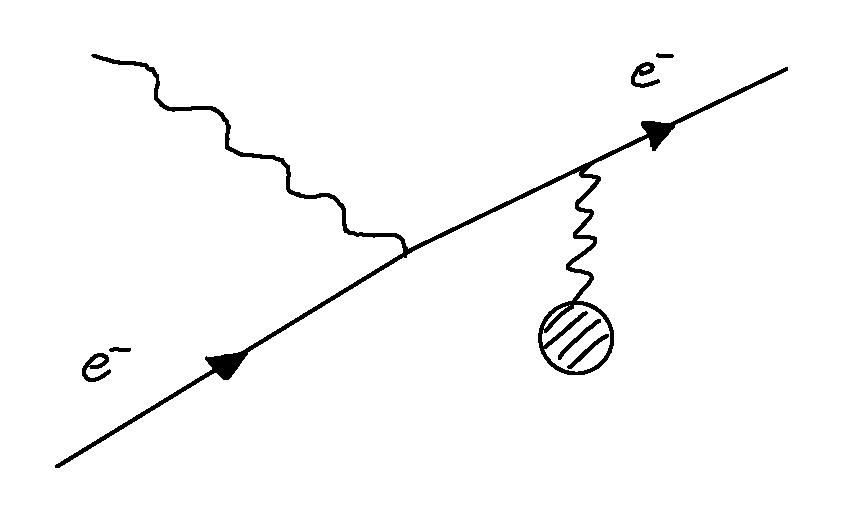
\includegraphics[width=\textwidth]{imgs/ep5-fig-3-5.pdf}
\captionof{figure}{Feynmandiagramm der Photoionisation\label{fig:3.5}}
\end{minipage}
\begin{minipage}[c]{.45\textwidth}
\captionsetup{type=figure}
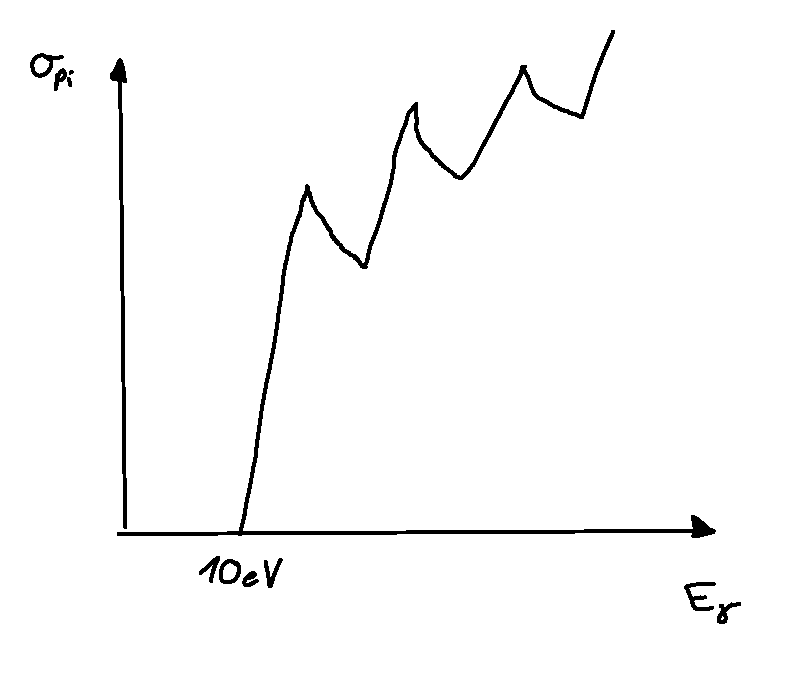
\includegraphics[width=\textwidth]{imgs/ep5-fig-3-6.pdf}
\captionof{figure}{Schematisches Absorptions-\\spektrum}
\end{minipage}

\tb{Compton-Streuung} (vgl. Abb.\ref{fig:3.7})\\
elastische Streuung, Energieübertrag auf $e^-$
\begin{align*}
\boxed{ \gamma + e^- \ra \gamma + e^- }
\end{align*}
Dominant für 30\,keV$\leq E_\gamma \leq$ 5\,MeV\\
$\Ra$ Wellenlänge ändert sich durch $\gamma$
\begin{align*}
\boxed{ \Delta \lambda = \frac{h}{m_e c} \left( 1 - \cos \theta \right) \ \ \ \forall E_\gamma }\\
\lambda_C= \frac{h}{m_e c} \approx 2.4\cdot 10^{-12}\,\mr{m}
\end{align*}
$\lambda_C$ Compton-Wellenlänge des Elektrons\\
Für $\nicefrac{E_\gamma}{m_e} \gg 1$:
\begin{align*}
\sigma_C \sim \alpha^2 \frac{1}{E_\gamma}\ln \left( \frac{2 E_\gamma}{m_e}\right)
\end{align*}

\begin{figure}[!ht]
\centering
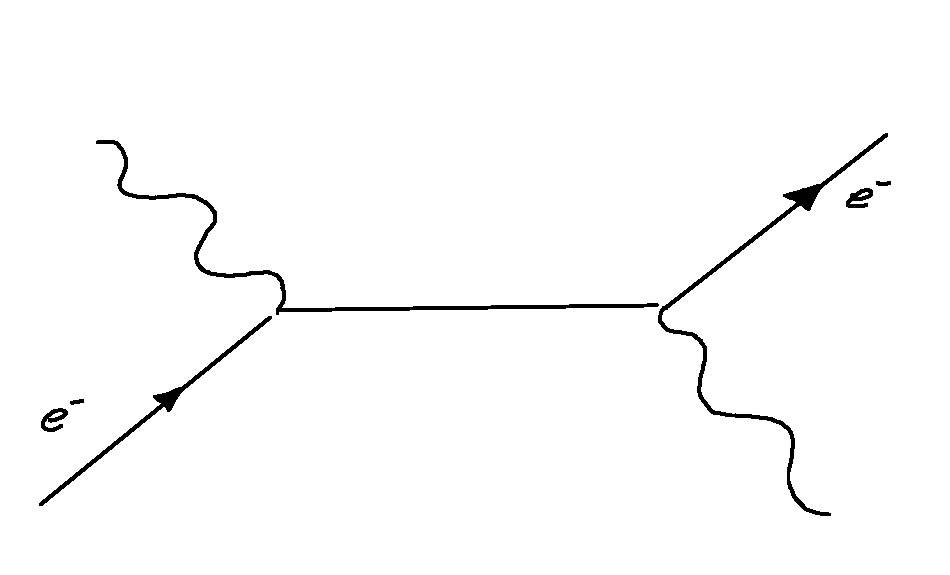
\includegraphics[width=.5\textwidth]{imgs/ep5-fig-3-7.pdf}
\caption{Feynmandiagramm der Compton-Streuung\label{fig:3.7}}
\end{figure}

 \tb{Paarbildung} (vgl. Abb.\ref{fig:3.8})
\begin{align*}
\boxed{ \gamma + \text{Kern} \ra e^+e^-+\text{Kern} }
\end{align*}
  Energieschwelle $E_\gamma > 2m_e \approx 1$\,MeV
\begin{align*}
\sigma_p \sim Z^2 \ln \frac{E_\gamma}{m_e}
\end{align*}
$\Ra$ dominant bei (sehr) hohen Energien

\begin{minipage}[c]{.45\textwidth}
\captionsetup{type=figure}
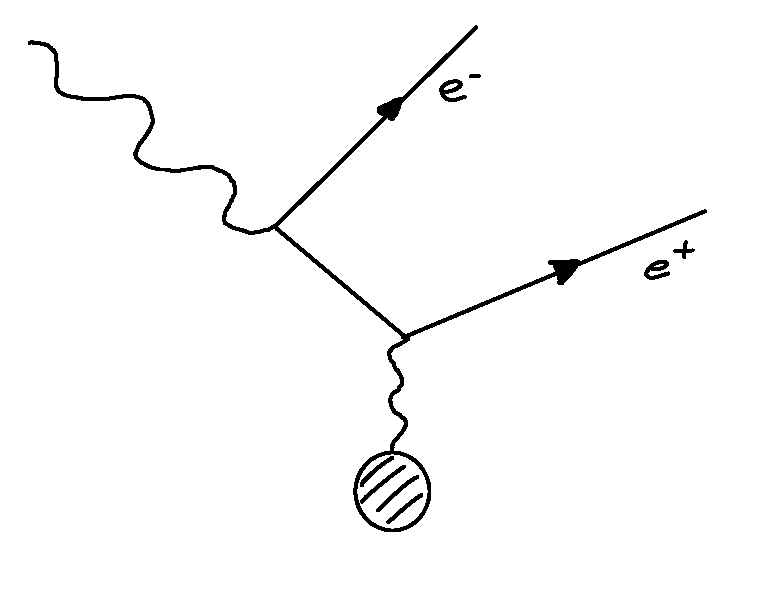
\includegraphics[width=\textwidth]{imgs/ep5-fig-3-8.pdf}
\captionof{figure}{Feynmandiagramm der\\ Paarbildung\label{fig:3.8}}
\end{minipage}
\begin{minipage}[c]{.45\textwidth}
\captionsetup{type=figure}
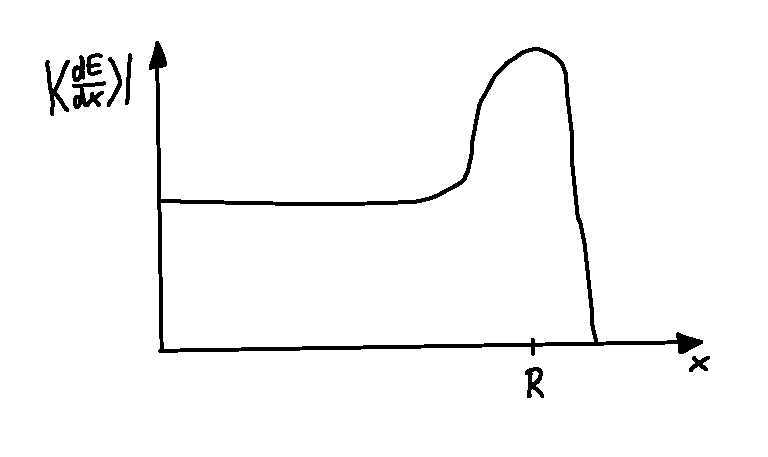
\includegraphics[width=\textwidth]{imgs/ep5-fig-3-9.pdf}
\captionof{figure}{Bragg-Peak visualisiert als\newline  Energieverlust für eine bestimmte Eindringtiefe\label{fig:3.9}}
\end{minipage}

\tb{Ionisation} (vgl. Abb. \ref{fig:3.9})

Am Ende des Abbremsvorgangs hoher Energieverlust $\sim \frac{1}{\beta^2}$ $\Rightarrow$ \glqq Bragg-Peak\grqq{}

\tb{Bremsstrahlung}
	\begin{align}
	\boxed{T+ \text{Kern}\rightarrow T+ \text{Kern}+\gamma}
	\end{align}
Energieverlust:
	\begin{align}
	\boxed{-\left\langle \dfrac{E}{x}\right\rangle_{\text{Brems}}=\frac{E}{x_0}}
	\end{align}
$x_0$: Strahlungslänge (materialabhängig)
	\begin{align}
	\boxed{\frac{1}{x_0}\sim \underbrace{nZ^2}_{\text{Material}} \cdot \frac{Z^2_s}{M^2}}
	\end{align}
$x_0=36\,cm$ für $e^-$ in $H_2O$ und $x_0=5,6\,mm$ für $e^-$ in $Pb$
\begin{itemize}
\item[$\ra$] $E(x)=E(x=0)\cdot e^{-\frac{x}{x_0}}$ ausschließlich Bremsstrahlung
\item[$\ra$] besonders stark für $e^-$ (kleine Masse)
\item[$\ra$] $x_0$ auch für Paarerzeugung: Mithilfe freier Weglänge $=\frac{7}{9}x_0$
\end{itemize}

	\begin{figure}[!ht]
	\centering
	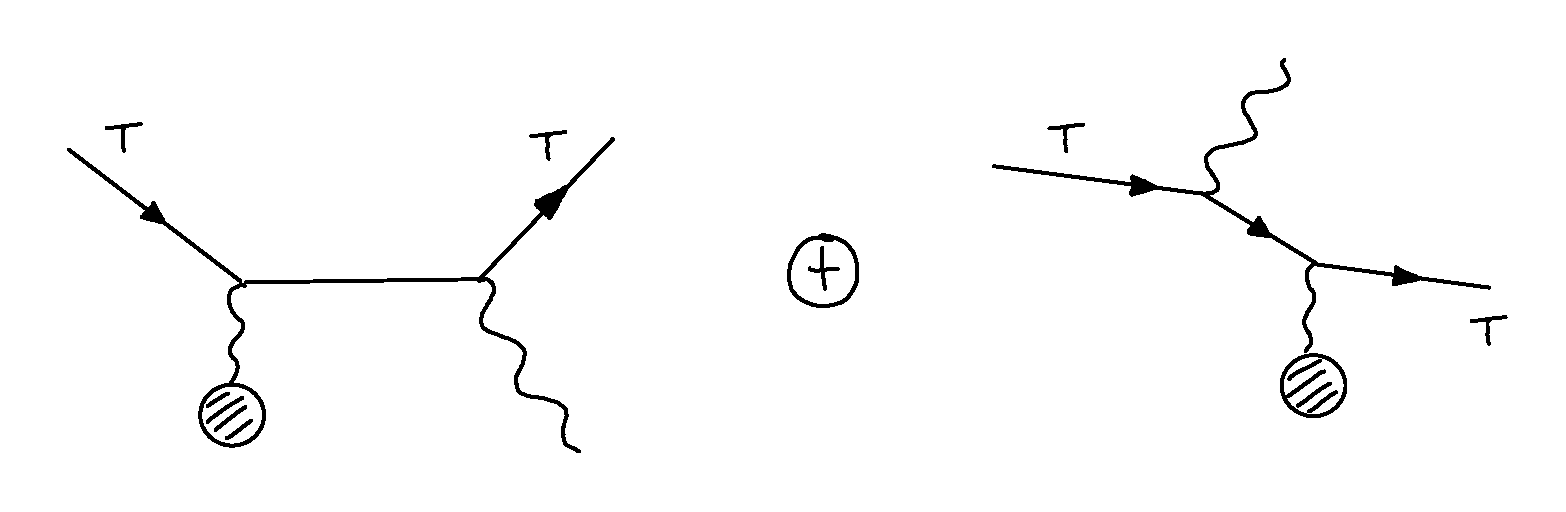
\includegraphics[width=.6\textwidth]{imgs/ep5-fig-3-10.pdf}
	\caption{Feynmandiagramme der Bremsstrahlung (für $T=e^-$, \glqq topologisch äquivalent zu Paarerzeugung\grqq ) \label{fig:3.10}}
	\end{figure}

\tb{Cherenkov-Strahlung}
	\begin{align}
	v_{\text{Teilch}}>v_{\text{Phase}}
	\end{align}
Durchgang geladener Teilchen durch transparente Medien (Brechungsindex n) mit $\beta >\frac{1}{n}$\\
Lichtemission. Aus Abb. \ref{fig:3.11} folgt geometrisch der Zusammenhang
\begin{align}
\boxed{cos\theta_c=\frac{1}{\beta n}}
\end{align}
\begin{itemize}
\item[$\ra$] Winkel für den Teilchennachweis verwendet
\item[$\ra$] Beitrag $2u\frac{dE}{dx}$ ist sehr klein
\end{itemize}
	\begin{figure}[!ht]
	\centering
	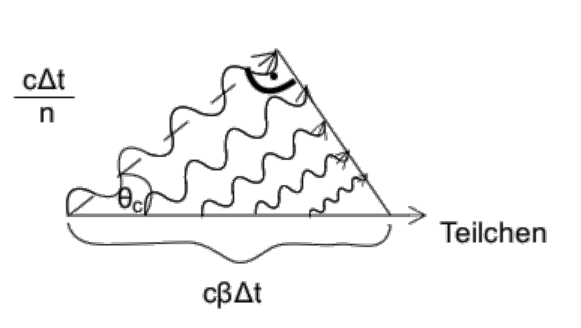
\includegraphics[width=.5\textwidth]{imgs/ep5-fig-3-11.pdf}
	\caption{Cherenkov-Strahlung mit charakteristischem Cherenkovkegel \label{fig:3.11}}
	\end{figure}

\textbf{Absorption von Photonen}
\begin{align}
\begin{split}
\Pa N =-W_a\cdot N =-\frac{\sigma \cdot N_T}{A}\cdot N=-\frac{\sigma n_T A\Pa x}{A}\cdot N\\
\Rightarrow \frac{dN}{dx}=-\underbrace{\sigma n_T}_{= \mu} N\\
\Rightarrow \boxed{N(x)=N_0 e^{-\mu x}}
\end{split}
\end{align}
\begin{compactitem}
\item[mit] $W_a$: Absorptionswahrscheinlichkeit
\item[] $\mu$ Absorptionskoeffizient
\end{compactitem}
\begin{itemize}
\item[$\ra$] Mittlere freie Weglänge
\begin{align}
\boxed{\lambda=\frac{1}{\mu}=\frac{1}{\sigma n_T}}
\end{align}
\item[$\ra$] Häufig angegeben:
\begin{align}
\boxed{\mu'=\frac{\mu}{\rho}=\frac{n_T}{\rho}\cdot \sigma=\frac{N_A}{M_m}\sigma}
\end{align}
\end{itemize}
	\begin{figure}[!ht]
	\centering
	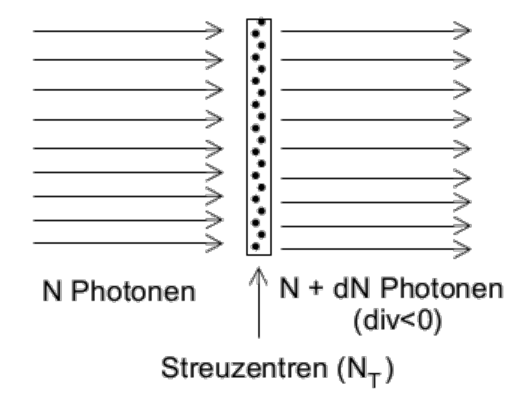
\includegraphics[width=.45\textwidth]{imgs/ep5-fig-3-12.pdf}
	\caption{Absorption von Photonen beim Durchgang durch ein Medium\label{fig:3.12}}
	\end{figure}

\section{Grundbegriffe der Dosimetrie}
Hier lediglich einige Grundbegriffe, \textbf{keine} Messverfahren.
Einfluss von Strahlenbelastung auf biologische Organismen
\begin{itemize}
\item[$\ra$] \textbf{Aktivität}
\begin{align}
\boxed{A=\left\langle\left|\frac{dN}{dt}\right|\right\rangle=
\frac{\text{mittlere Zahl von Zerfällen}}{\mr s}}
\end{align}
\begin{itemize}
\item[$\ra$] charakterisiert Stärke einer Strahlungsquelle
\item[$\ra$] $[A]=\nicefrac{1}{\mr{s}}=\mr{Bq}=$Becquerel
\item[$\ra$] Bsp.: $^{40}K$-Zerfall im menschlichen Körper $A\sim 10^4\,Bq$ (ca. $10\,\%$ der nat. Strahlenbelastung)\\
\end{itemize}
\item[$\ra$] \textbf{Strahlungsleistung} $A\cdot E$, mit $E$ als freigesetzter Energie pro Zerfall
\item[$\ra$] \textbf{Energiedosis}\\
In Absorber deponierte Energie/Masse
\begin{align}
\boxed{D=\frac{dE}{dM}=\frac{1}{\rho}\frac{\Pa E}{\Pa V},[D]=\mr{\frac{J}{kg}}=\mr{Gy}=\text{Gray}}
\end{align}
(alt: $1\,\mr{Gy}=100\,\mr{rad}$)
\begin{itemize}
\item[$\ra$] Produktion von Sekundärteilchen, chemische Radikale
\item[$\ra$] Schädigung der DNA $\rightarrow$ Mutationen
\item[$\ra$] $\alpha-,\beta-,\gamma-$Strahlung ($\rightarrow$ Kap 5) wirken sehr unterschiedlich schädigend
\end{itemize}
\item[$\ra$]\textbf{Äquivalentdosis}
\begin{align}
\begin{split}
H=D\cdot Q\\
[H]=\mr{\frac{J}{kg}}=\mr{Sv}=\text{Sievert}\\
Q=\begin{cases}
1 & \text{für } e^\pm,\gamma\\
10 & \text{für schnelle }n \\
20 & \text{für }\alpha-\text{Teilchen, Kerne}
\end{cases}
\end{split}
\end{align}
$Q$ = relative, biologische Wirksamkeit=\glqq Qualitätsfaktor\grqq\\
(alt: $1\,\mr{Sv}=100\,\mr{rem}$)
\item[$\ra$] \textbf{Typische Dosen}\\
Natürliche Strahlenbelastung (Gestein): $1\,\mr{\frac{mSv}{a}}$\\
Transatlantikflug: $50-100\,\mu \mr{Sv}$\\
Computertomographie: $10\,\mr{mSv}$\\
Höchstgrenze Strahlenschutzverordnung $20\,\mr{\frac{mSv}{a}}$\\
Letale Dosis: $6\,\mr{Sv}$

Achtung: Gesundheitswirkung:
\begin{itemize}
\item[$\ra$] hängt davon ab, in welchem Organ Strahlung deponiert wird
\item[$\ra$] ist besonders stark bei inkorporierten Quellen
\end{itemize}
\end{itemize}
\chapter{Atomkerne und Kernmodelle}
\begin{itemize}
\item[$\ra$] Geometrie von Kernen
\item[$\ra$] Kernzusammensetzung
\item[$\ra$] Modelle für Kernmassen etc.
\end{itemize}

\section{Kernradien und Formfaktor}
\begin{itemize}
\item Experimentelle Untersuchung der Kerngrößen durch Streuexperimente
\begin{align}
\begin{matrix}
(e^- , \alpha) & A & \ra & (e^- , \alpha)\ A & \text{(el. Ladung)}\\
\underbrace{\ n \ } & \underbrace{\ A \ } & \underbrace{\ \ra \ } & n\ A & \text{(Massendichte)} \\
 \text{\glqq Sonde\grqq} & \text{Kern} & \text{el. Streuung} & & 
\end{matrix}
\end{align}
Typische Energien: $E_\mr{kin}\sim 1 \text{ bis } 100\,\mr{MeV}$\\
Gute Näherung: $E_\mr{kin} \ll M_A$\\
$\Rightarrow$ Energieübertrag auf Kern ist vernachlässigbar
\begin{figure}[!ht]
	\centering
	\begin{tikzpicture}
	\begin{feynman}
	\vertex (a1);
	\node[right = 3cm of a1, blob] (a2) {A};
	\vertex[above right = 3cm of a2] (c1);
	\vertex[below right = 3cm of a2] (d1);
	
	\diagram*{
	(a1) -- [fermion, edge label = {$e$,$\alpha$,$\vec p$}] (a2),
	(a2) -- [fermion, edge label = {$e$,$\alpha$,$\vec p^{\;\prime}$}] (c1),
	(a2) -- [fermion] (d1)
	};
	\end{feynman}
	\end{tikzpicture}
	\caption{Energieübertrag auf Kern durch Stoß\label{fig:4.1}}
\end{figure}
\begin{align}
E^A_\mr{kin}=\frac{q^2}{2M_A} \ll \frac{p^2}{2m_{\alpha,e}}=E^{\alpha,e}_\mr{kin}
\end{align}
(Achtung: für $\alpha$-Streuung an leichten Kernen nicht gültig, da $\labs\vec{p}\rabs = \labs \vec{p}^\prime\rabs$)\\
\begin{figure}[!ht]
	\centering
	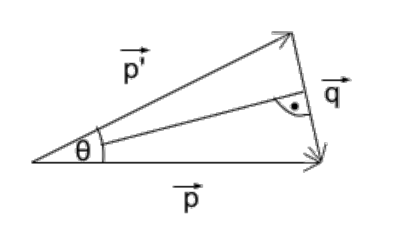
\includegraphics[width=.35\textwidth]{imgs/ep5-fig-4-2.pdf}
	\caption{Impulsübertrag $q$ eines elastisch gestreuten Teilchens \label{fig:4.2}}
	\end{figure}
Aus Abb. \ref{fig:4.2} ergibt sich für $q^2= (\vec p - \vec{p}^\prime)^2$:
\begin{align}
q^2=\lb 2\labs \vec{p}\rabs \sin\frac{\theta}{2}\rb ^2 = \lb  2 p \sin \frac{\theta}{2}\rb ^2
\end{align}
\begin{figure}[!ht]
	\centering
	\begin{tikzpicture}
    \begin{feynman}
    \vertex (a1);
    \vertex [below right= 3cm of a1] (a2);
    \vertex [above right= 3cm of a2] (a3);
    \node [below= of a2, blob] (b2);
    
    \diagram*{
    (a1) -- [fermion, edge label = $e^-$] (a2),
    (a2) -- [fermion, edge label = $e^-$] (a3),
    (a2) -- [photon, edge label = $\gamma$] (b2),
    };
    \end{feynman}
    \end{tikzpicture}
	\caption{Feynman-Diagramm der elektromagnetischen Wechselwirkung mit dem Kern $A$\label{fig:4.3}}
	\end{figure}
    
$\Rightarrow$ der WQ ist elm. (vgl.Abb.\ref{fig:4.3}), daher Coulomb-Streuung
\begin{align}
\begin{split}
\frac{\Pa \sigma}{\Pa \Omega}\sim (e^2)(Ze^2)\frac{1}{q^4}\sim Z^2\alpha^2\frac{1}{q^4}\\
q^2 \text{ in } q^4 \text{ gegeben durch } q^2=\underbrace{\lb E-E^\prime \rb ^2}_{=0}-\vec{q}^2\\
\Rightarrow q^2=-4p^2\sin^2\frac{\theta}{2}\\
\Rightarrow \boxed{\frac{d\sigma}{d\Omega}\sim \frac{Z^2\alpha^2}{16p^4 \sin^4 \frac{\theta}{2}}}\\
\sim\text{ Rutherford-WQ}
\end{split}
\end{align}
\begin{itemize}
\item[$\ra$] starke $p$- und $\theta$-Abhängigkeit
\item[$\ra$]  maximales $\labs \vec{q} \rabs$ für $\theta=180^{\circ}$
\begin{itemize}
\item[$\ra$]  stärkste Annäherung
\item[$\ra$]  kleinster WQ
\end{itemize}
\item[$\ra$]  $e^-$ relativistisch
\item[$\ra$]  $\alpha$ nicht-relativistisch
\end{itemize}

\item Was ändert sich, wenn A ausgedehnte Ladungsverteilung $\rho\lb \vec{r}\rb $ hat?
\begin{align}
\left. \frac{\Pa \sigma}{\Pa \Omega}\right|_\mr{Coul}\rightarrow \left. \frac{\Pa \sigma}{\Pa \Omega}\right|_\mr{Coul}\cdot \left|F\lb \vec{q}\rb \right|^2
\end{align}

Hierbei ist der Formfaktor $F\lb \vec{q}\rb $ eingeführt worden. Er errechnet sich als Fouriertransformierte der Ladungsverteilung.
\begin{align}
\boxed{F\lb \vec{q}\rb =\frac{1}{Ze}\int e^{i\vec{q}\vec{r}}\rho \lb \vec{r}\rb  \Pa^3 r}
\end{align}
(Offenbar gleich zu Beugungseffekt: QM Störungsrechnung (mehr in Kap. 6))
\begin{itemize}
\item Messung von $\frac{\Pa \sigma}{\Pa \Omega}$
\item[$\ra$] Bestimmung von $\labs F\lb \vec{q}\rb  \rabs ^2$
\item[$\ra$] Bestimmung von $\rho(\vec{r})$
\end{itemize}

Ergebnis für $\rho(\vec{r})=\rho\lb r\rb $ bei homogener Ladungsverteilung (Abb. \ref{fig:4.4}):
\begin{align}
\boxed{\rho\lb r\rb =\frac{\rho_0}{1+e^{\frac{r-a}{b}}}}
\end{align}
Typische Werte der Parameter $a$, $b$:
\begin{align}
\boxed{a=1.07 \mr{A^{\nicefrac{1}{3}}\,fm} \qquad b=0.54\,\mr{fm}}
\end{align}
Gleiches $\rho_0$ homogener Ladungsverteilung, scharfer Rand:
\begin{align*}
\boxed{R_A=1.21 A^{\nicefrac{1}{3}}\,\mr{fm}}
\end{align*}
\end{itemize}
\begin{figure}[!ht]
	\centering
	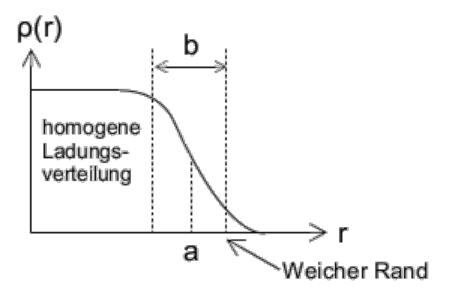
\includegraphics[width=.35\textwidth]{imgs/ep5-fig-4-4.pdf}
	\caption{Homogene Ladungsverteilung in einem Teilchen/Kern\label{fig:4.4}}
	\end{figure}

\section{Kernaufbau und Bindungsenergie}
Ein Atomkern besteht aus
\begin{align*}
\boxed{ \begin{matrix}
Z & \text{Protonen (p)}\\ N & \text{Neutronen (n)}\\ Z + N = A & \text{Nukleonen (p+n)}
\end{matrix} \ A: \ \text{Massenzahl} }
\end{align*}
Schreibweise: $^A_Z X_N$ mit $X$ als Elementsymbol\\
z.B. $^{12}_6 C_6$, auch $^{12}_6 C$, $^{12}C\ \lsb C12,12C\rsb $ \\
\begin{figure}[!ht]
	\centering
	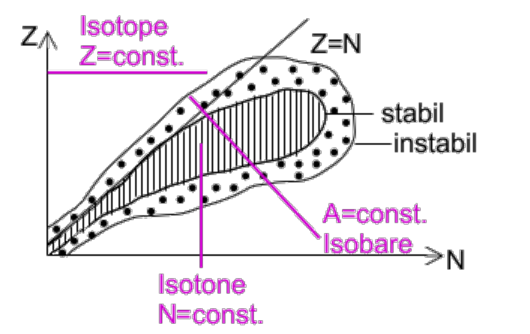
\includegraphics[width=.5\textwidth]{imgs/ep5-fig-4-5.pdf}
	\caption{Nuklidkartenskizze in der N-Z-Ebene \label{fig:4.5}}
	\end{figure}

\begin{itemize}
\item[$\ra$] \textbf{Bindungsenergie}\\
Energie $\mathcal{O}(10\,MeV)$ nötig, um Nukleonen aus Kern zu lösen.\\
Gesamte Bindungsenergie eines Atoms:
\begin{align}
E_B(A,Z)=\underbrace{E(Zp+Nn+Ze^-)}_{ZM_p+NM_n+Zm_e}-\underbrace{E(^A_Z X_N)}_{M(^A_Z X_N)=M(A,Z)}
\end{align}
Oft:
\begin{align}
\boxed{\Delta M=-E_B \,\widehat{=}\, \text{Massendefekt}}
\end{align}
Messung von $E_B$ erfordert präzise Messung von Atom/Kernmassen
\begin{itemize}
\item[$\Ra$] Massenspektroskopie (Ablenkung in $E$- und $B$-Feldern, $\frac{\Delta M}{M}\sim \mathcal{O}(10^{-6})$)
\item[$\Ra$] Ergebnis: $E_B \simeq 1\%$ von $M(A,Z)$
\item[$\lt$] viel größer als bei elm. WW ($10^{-6}$ bis $10^{-8}$ bei Atomen)
\end{itemize}
\begin{figure}[!ht]
	\centering
	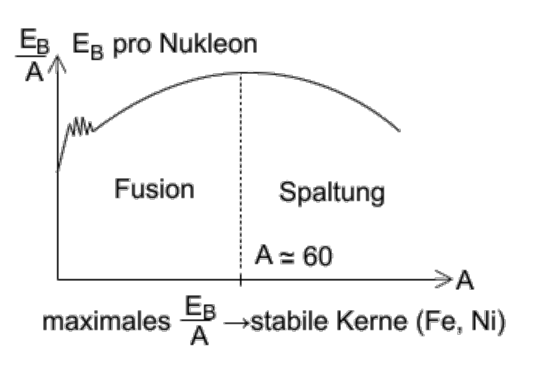
\includegraphics[width=.5\textwidth]{imgs/ep5-fig-4-6.pdf}
	\caption{Bindungsenergie pro Nukleon über die Nukleoenenzahl aufgetragen. Erkennbar ein Maximum, zu welchem Kerne fusioniert werden können zur Energiegewinnung und oberhalb dessen Kerne gespalten werden \label{fig:4.6}}
	\end{figure}
\begin{itemize}
\item[$\ra$] stabile Kerne mit $A\leq 60$:\\
Energiegewinn durch Fusion (Sonne!)
\item[$\ra$] stabile Kerne mit $A>60$:\\
Energiegewinn durch Spaltung (Kernkraftwerke, -waffen)
\end{itemize}
Können wir $\frac{E_B}{A}$ verstehen?
\begin{itemize}
\item[$\ra$] wenn starke WW langreichweitig (wie Coulomb)\\
$E_B\sim \frac{1}{2}A(A-1)\leftarrow$ Zahl der Nukleonenpaare\\
Aber: $E_B\sim A$
\item[$\Ra$] $\boxed{\text{starke WW kurzreichweitig (Nukleon \glqq sieht\grqq nur nächste Nachbarn)}}$
\end{itemize}
\end{itemize}

\section{Tröpfchenmodell und Weizsäcker-Massenformel}
Das sogenannte Tröpfchenmodell war das erste Modell der Kernphysik zur Beschreibung deren Eigenschaften. Da es das erste ist, ist es auch durchaus inkomplett.\footnote{Der Physiker Weizsäcker ist der Bruder des ehemaligen Bundespräsidenten}

\begin{itemize}
\item[$\rightarrow$] Kerndichte $\approx \ const.$
\item[$\rightarrow$] Kerne sphärisch
\item[$\rightarrow$] \glqq Verdampfungsenergie\grqq{} $\sim \ M$
\item[$\Rightarrow$] Wie bei (Wasser)tröpfchen!
\end{itemize}
Modell aus 1930er Jahren (formuliert von Weizsäcker, Williams, Gamov, Bohr):
\begin{align}
\boxed{ E_B = a_v A - a_s A^{\nicefrac{2}{3}} - a_c \frac{Z^2}{A^{\nicefrac{1}{3}}} - a_a \frac{(N-Z)^2}{A} - \frac{\delta}{A^{\nicefrac{1}{2}}}}
\end{align}
\begin{compactitem}
\item[mit] $a_vA \ =$ \textbf{Volumenterm}\\
$a_v$ Bindung der Nukleonen an ihre Nachbarn
\item[] $-a_sA^{\nicefrac{2}{3}}\ = $ \textbf{Oberflächenterm}\\
$a_s \approx 18\,$MeV, Nukleonen an der Oberfläche haben weniger Nachbarn, Effekt $\sim R^2 \sim A^{\nicefrac{2}{3}}$ mit $R^3 \sim A$
\item[] $-a_c \frac{Z^2}{A^{\nicefrac{1}{3}}} \ =$ \textbf{Coulombterm}\\
$a_c \approx 0.7\,$MeV, Energie einer homogen geladenen Kugel $\sim \frac{Q^2}{R}$ (Abstoßung der p)
\item[] $-a_a\frac{(N-Z)^2}{A}\ = $ \textbf{Asymmetrieterm}\\
$a_a \approx 23$\,MeV, p, n haben Spin $\nicefrac{1}{2}$ (Fermionen)\\
$\Rightarrow$ Pauli-Prinzip
\item[] $-\frac{\delta}{A^{\nicefrac{1}{2}}} \ =$ \textbf{Paarungsterm},
\begin{align}
\delta = \left\lbrace \begin{matrix} -11\,\mathrm{MeV}& gg\\ 0 & gu,\ ug\\ +11\,\mathrm{MeV} & uu \end{matrix}\right.
\end{align}
$u=$ ungerade, $g=$ gerade, $gg=$ $N$ gerade und $Z$ gerade
\end{compactitem}

\begin{figure}[!ht]
\centering
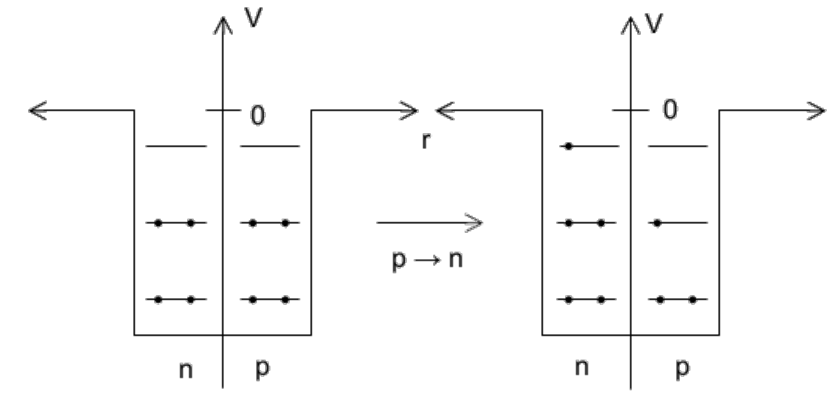
\includegraphics[width=.5\textwidth]{imgs/ep5-fig-4-7.pdf}
\caption{Umwandlung eines Protons in ein Neutron \label{fig:4.7}}
\end{figure}

Gepaarte Nukleonen sind stärker gebunden als \glqq einzelne\grqq{}
\begin{itemize}
\item[$\leadsto$] Modell kann $E_B(A,Z)$ grob beschreiben (insbesondere auch die Region der stabilen Kerne).
\item[$\rightarrow$] Aber:
\begin{compactitem}
\item QM-Effekte \glqq von Hand\grqq
\item Keine Dynamik (Nukleonen im Kern bewegen sich: $\Delta x \cdot \Delta p \gtrsim \hbar$)
\item Keine feineren Strukturen in $E_B(A,Z)$
\item keine Aussagen über Spin, magn. Moment, Parität
\end{compactitem}
\item[$\leadsto$] Interessant: Mit Gravitations- statt Coulombterm $\rightarrow$ Neutronenstern $\approx$ stabile Lösung
\end{itemize}

\section{Das Fermigasmodell}
\begin{figure}[!ht]
\centering
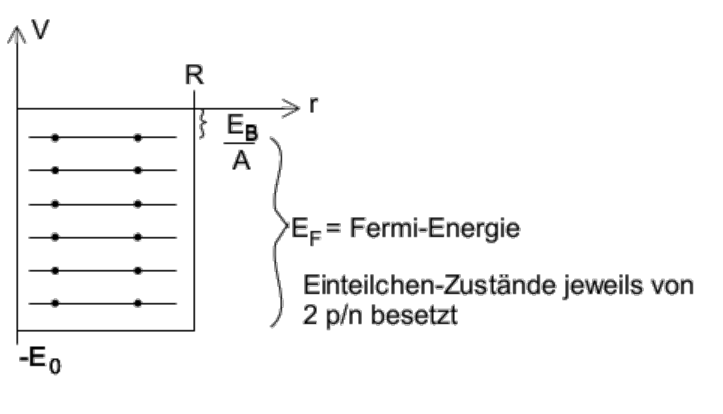
\includegraphics[width=.5\textwidth]{imgs/ep5-fig-4-8.pdf}
\caption{Potentialtopf nach dem Fermigasmodell \label{fig:4.8}}
\end{figure}
Nukleonen gebunden durch WW mit allen anderen Nukleonen.
\begin{itemize}
\item[$\rightarrow$] Effektives Potential
\item[$\rightarrow$] Einfache Näherung: Kastenpotential
\item[$\leadsto$] Wie groß sind $E_F$, $p_F= \sqrt{2M_NE_F}$, $E_0$, $\nicefrac{E_B}{A}$
\item[$\leadsto$] Achtung: $E_0^{(n)} < E_0^{(p)}$ wegen Coulomb-WW der $p$
\begin{compactitem}
\item[$\leadsto$] zunächst vernachlässigt
\end{compactitem}
\end{itemize}
Erinnerung an Quantenmechanik:
\begin{center}
$\boxed{\text{QM: 1 Zustand pro Phasenraumvolumen }(\Delta x\, \Delta p)^3 = \mathrm{h}^3}$
\end{center}
Gesamtes Phasenraumvolumen im Kern:
\begin{align}
\Delta x^3 \rightarrow V_K = \frac{4 \pi}{3} R_n^3\\\Delta p^3 \rightarrow V_p = \frac{4 \pi}{3}p_F^3
\end{align}
\begin{itemize}
\item[$\Rightarrow$] Zahl der Zustände
\begin{align}
\boxed{n= \frac{1}{h^3} \lb  \frac{4\pi}{3} R_n^3\rb \lb \frac{4\pi}{3} p_F^3\rb = \frac{N+Z}{4}= \frac{A}{4}}
\end{align}
\begin{compactitem}
\item[mit] $R_n = R_0 A^{\nicefrac{1}{3}}$, $R_0 = 1.21$\,fm
\end{compactitem}
\begin{align}
\Rightarrow\ \boxed{p_F = \frac{\hbar}{R_0}\lb \frac{9 \pi}{8}\rb ^{\nicefrac{1}{3}} = \frac{197\,\mathrm{MeV\,fm}}{1.21\,\mathrm{fm}}\lb \frac{9 \pi}{8}\rb ^{\nicefrac{1}{3}} = 250\,\mathrm{MeV}}
\end{align}
\item[$\leadsto$] hoher Impuls, etwa wie von Unschärferelation erwartet $\lb \Delta p \sim \frac{\hbar}{R_0}\rb $
\item[$\leadsto$] durch $eA$-Streuung bestätigt
\begin{align}
\lt \ \boxed{{E_F} = \frac{p_F^2}{2M_N} \approx 33\,\mathrm{MeV} \Rightarrow\ E_0 = E_F+ \frac{E_B}{A} \approx 40 \, \mathrm{MeV}}
\end{align}
\item[$\leadsto$] Genauer: mit Coulombpotential
\item[$\leadsto$] Rechnung mit $p_F^{(n)} \neq p_F^{(p)}$ ergibt:
\begin{align}
E_\mathrm{min}^\mathrm{tot} \sim A + \frac{5}{9} \frac{(N-Z)^2}{A}
\end{align}
zweiter Summand erklärt Asymmetrieterm
\item[$\leadsto$] Paarungsterm: Beispiel $^{40}$K, $^{40}$Ca
\end{itemize}

\begin{figure}[!ht]
\centering
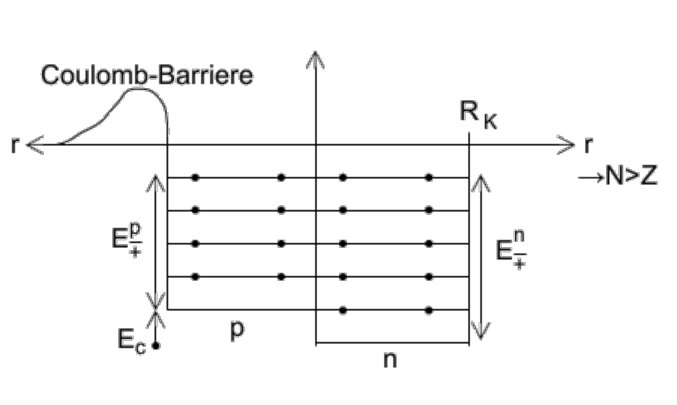
\includegraphics[width=.5\textwidth]{imgs/ep5-fig-4-9.pdf}
\caption{Potentialtopf mit Berücksichtigung der verschiedenen Bindungsenergien für Neutronen und Protonen \label{fig:4.9}}
\end{figure}

\begin{figure}[!ht]
\centering
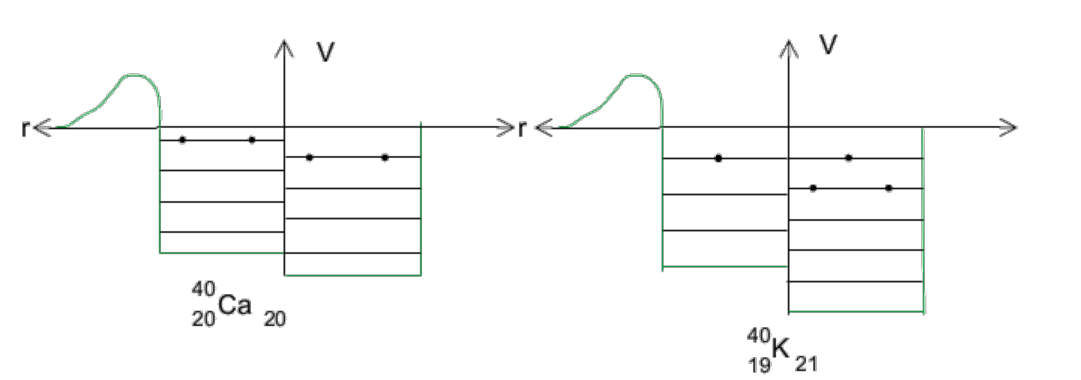
\includegraphics[width=.5\textwidth]{imgs/ep5-fig-4-10.pdf}
\caption{Potentialtopf am Beispiel für Kalium und Calcium \label{fig:4.10}}
\end{figure}

Fermigasmodell:
\begin{compactitem}
\item einfachstes QM-Modell von Kernen
\item erklärt qualitativ QM-Terme in Weizsäcker-Formel
\item aber: keine Vorhersagen zu Spin, magn. Moment und Parität
\end{compactitem}

\section{Das Schalenmodell}
Einteilchen-Wellenfunktion in effektivem Kernpotential $\lt$ Schrödinger-Gleichung
\begin{itemize}
\item \textbf{Potential}\\
$V_S (r) \sim \varrho_K (r) \ =$ Nukleonendichte
\begin{figure}[!ht]
\centering
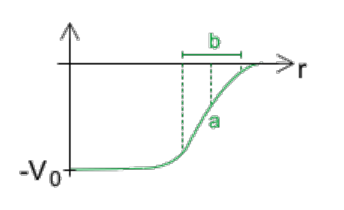
\includegraphics[width=.5\textwidth]{imgs/ep5-fig-4-11.pdf}
\caption{Skizze des Woods-Saxon-Potentials \label{fig:4.11}}
\end{figure}
\begin{align}
\boxed{
V_S(r) = -V_0 \frac{1}{1+e^{\nicefrac{(r-a)}{b}}}
}\\
\sim \text{ Woods-Saxon-Potential}\nonumber
\end{align}
Achtung:
\begin{compactitem}
\item effektives Potential
\item keine zentrale \glqq Kraftquelle\grqq
\item Kräfte \textbf{viel} stärker als in Atom
\end{compactitem}
\item[$\lt$] SG analytisch nicht lösbar
\item[$\lt$] Näherung als harmonischer Oszillator\\
$V_S\lb r\rb  = -V_0 + \frac{1}{2}kr^2, \ r \leq R_k$
\item[$\lt$] In jedem Fall: $V_S\lb  \vec{r}\rb  = V_S(r)$ (sphärisch symmetrisch)
\begin{compactitem}
\item[$\Ra$] Winkelanteil $Y_{lm} (\vartheta, \varphi )$
\item[$\Ra$] Hauptquantenzahl $n$
\item[$\Ra$] $E= \underbrace{E(n,l)}_{2(2l+1)\text{-fach entartet}}$\\
Vorfaktor 2 durch 2 Fermionen pro WF, $2l+1$ Werte für $m$
\end{compactitem}
\begin{align}
\boxed{ E(n,l) = \lb N+\frac{3}{2}\rb  E_0 + \underbrace{\Delta E \lb  n,l\rb }_{=0\text{ für h.O.}}}\\
N=2(n-1)+l\nonumber \\
\Delta E(n,l) = \llb \begin{matrix} \text{klein für kleine } n \text{ und große } l \\ \text{groß für große } n \text{ und kleine } l \end{matrix} \right.
\end{align}
\item[$\Ra$] Baue \glqq Schalen\grqq{} (wie in Atomphysik)
\begin{table}
\centering
\begin{tabular}[!ht]{c|cccc}
$N$ & $nl$ & $2(2l+1)$ & $\sum 2(2l+1)$ & beob?\\
\hline
0 & 1s & 2 &2 & Ja\\
1 & 1p & 6 & 8 & Ja\\
2 & 1d & 10 & 18 & Nein\\
2 & 2s & 2 & 20 & Ja\\
3 & 1f & 14 & 34 & Nein\\
3 & 2p & 6 & 40 & Nein
\end{tabular}
\end{table}
\item[$\ra$] Was fehlt? LS-Kopplung\\
\textbf{Wichtig:} Erfolgt durch \textbf{starke} WW $\Ra$ großer Beitrag zu $V(r)$
\begin{compactitem}
\item[$\lt$] $V_{LS}(r) = \underbrace{\lla V_{LS}\rra}_{<0}\lla \vec{l}\vec{s}\rra$
\item[$\lt$] $\vec{j} = \vec{l} + \vec{s}$ wird bevorzugt maximal\\
$\Ra \ \lla \vec{l}\vec{s}\rra = \frac{1}{2} \lsb  \lla \vec{j}^2\rra - \lla \vec{l}^2\rra - \lla \vec{s}^2 \rra \rsb $\\
$\lla \vec{j}^2\rra = j(j+1)$, $\lla \vec{l}^2\rra = l(l+1)$, $\lla \vec{s}^2\rra = s(s+1)$
\end{compactitem}
\begin{align}
\Ra \ \boxed{ \lla \vec{ls} \rra = \llb \begin{matrix}
\frac{l}{2} \text{ für } j = l+\frac{1}{2}\\
-\frac{l+1}{2} \text{ für } j = l - \frac{1}{2}
\end{matrix} \right. }
\end{align}
\item[$\Ra$] Termschema mit besonders großen Lücken bei
\begin{align*}
\boxed{
\begin{matrix}
 & \text{He} & \text{O} & \text{Ca} & \text{Ni} & \text{Sn} & \text{Pb}\\
 Z = & 2, & 8, & 20, & 28, & 50, &82\\
 N= & 2, & 8, & 20, & 28, & 50, & 82, & 126
\end{matrix}
}
\end{align*}
sogenannte \glqq magische Zahlen\grqq{} $\lt$ Schalen
\item[$\Ra$]  Kerne mit abgeschlossenen Schalen besonders stabil (\glqq magisch\grqq)
\item[$\Ra$] Noch stabiler: \glqq doppelt-magische\grqq{} Kerne:\\
$\boxed{^4_2\text{He}_2, \ ^{16}_8\text{O}_8, \ ^{40}_{20}\text{Ca}_{20}, \ ^{48}_{20}\text{Ca}_{28}, \ ^{208}_{82}\text{Pb}_{126}}$
\item[$\Ra$] Nomenklatur $nL_j$\\ z.B. 2$P_{\nicefrac{3}{2}}$
\item[$\Ra$] Wie in Atomphysik: abgeschlossene Schalen haben Spin, magnetisches Moment $=0$
\item[$\Ra$]  Verhalten von Kernen mit 1 zusätzlichen Nukleon wird durch dieses bestimmt (\glqq Leuchtnukleon\grqq)\\
\textbf{Beispiel:}
\begin{align*}
^{17}_8\text{O}_9, \ Z= 8:\qquad \underbrace{\underbrace{(1S_{\nicefrac{1}{2}})}_2 \underbrace{(1P_{\nicefrac{3}{2}})}_4 \underbrace{(1P_{\nicefrac{1}{2}})}_2}_{\text{abgeschlossen}}\\
N= 9 :\qquad (1S_{\nicefrac{1}{2}})(1P_{\nicefrac{3}{2}})(1P_{\nicefrac{1}{2}}) + (1D_{\nicefrac{5}{2}})\\
\Ra \text{ Spin} \lb  ^{17}_8\text{O}_9\rb  = \underbrace{\text{Spin}\lb  ^{16}_8\text{O}_8\rb }_{=0} + \frac{5}{2}\\
\Ra \text{ magn. Mom.: } \mu\lb  ^{17}_8\text{O}_9\rb  = \mu\lb  ^{16}_8\text{O}_8\rb  + \mu_n  = -1.91\mu_N
\end{align*}
\end{itemize}

\chapter{Kernzerfälle und -spaltung}
\begin{compactitem}
\item Verschiedene Zerfallsmoden
\item (Historisch) erster Zugang zur schwachen WW
\item Kernspaltung $\lt$ Kettenreaktionen
\end{compactitem}
\section{\texorpdfstring{$\alpha$}{}-Zerfall von Kernen}
Emission eines $\alpha$-Teilchens $= \ ^4_2\text{He}_2$-Kern (He-Kern doppelt magisch)
\begin{align}
\boxed{
^A_Z X_N \ra ^{A-4}_{Z-2} Y_{N-2} + \alpha
}
\end{align}
\begin{figure}[!ht]
\centering
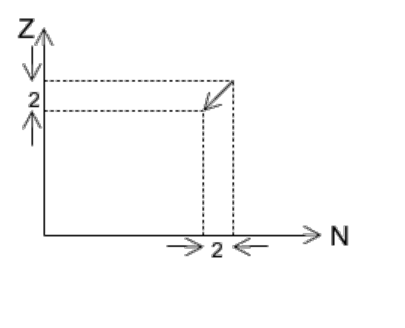
\includegraphics[width=.4\textwidth]{imgs/ep5-fig-5-1.pdf}
\caption{$\alpha$-Zerfall in der Nuklidebene \label{fig:5.1}}
\end{figure}
\begin{itemize}
\item Energiebilanz:
\begin{align}
\boxed{
M(A,Z) = M(A-4, Z-2) + M_\alpha + Q
}
\end{align}
$Q\ =\ Q$-Wert
\item[$\lt$] Zerfall ist möglich, wenn $Q>0$
\item[$\lt$] Wegen $M_\alpha \overset{\text{i.d.R.}}{\ll} M(A-4, Z-2)$ ist $Q\approx T_\alpha$
\item[$\lt$] Bei p, n-Emission ist $Q$ um $E_B(\alpha)$ kleiner
\begin{compactitem}
\item[$\lt$] kommt nur sehr selten vor
\end{compactitem}
\item[$\lt$] 2-Körper-Endzustand
\begin{itemize}
\item[$\Ra$] für gegebenen Zerfall hat $T_\alpha$ immer den gleichen Wert
\item[$\Ra$] \glqq Linienspektrum\grqq
\end{itemize}
Deutung/Interpretation:\\
Im Kern formiert sich $\alpha$-Teilchen, das Kern durch Tunnelvorgang verlassen kann

\begin{minipage}[c]{.45\textwidth}
\captionsetup{type=figure}
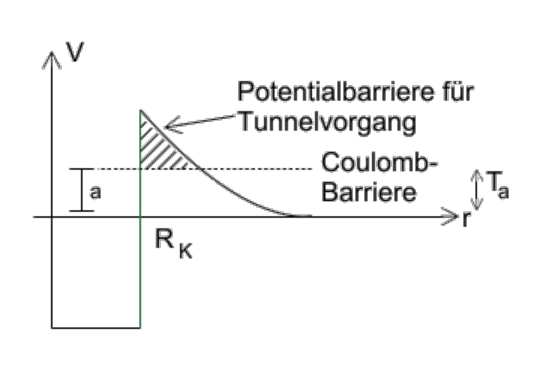
\includegraphics[width=\textwidth]{imgs/ep5-fig-5-2.pdf}
\captionof{figure}{Potentialtopf mit Coulomb- und Tunnelbarriere \label{fig:5.2}}
\end{minipage}
\begin{minipage}[c]{.45\textwidth}
\captionsetup{type=figure}
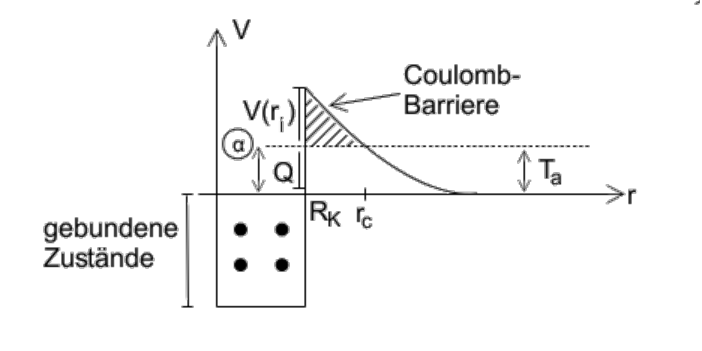
\includegraphics[width=\textwidth]{imgs/ep5-fig-5-3.pdf}
\captionof{figure}{Tunnelbarriere für ein $\alpha$-Teilchen aus dem Kernpotential \label{fig:5.3}}
\end{minipage}

\item \textbf{Tunnelwahrscheinlichkeit} für Barriere mit Breite $\Pa r$ und Höhe $v(r)$
\begin{align}
\boxed{
\Pa p_i = \exp \left( - \frac{2}{\hbar} \sqrt{2 m_\alpha (v(r) -Q)}\ \Pa r \right)
}
\end{align}
Damit ergibt sich die gesamte Tunnelwahrscheinlichkeit zu 
\begin{align}
P \ = \prod_i \Pa p_i = \exp \left( - \frac{2}{\hbar} \int_{R_k}^{r_C} \sqrt{ 2 m_\alpha \left(v(r) -Q\right)} \Pa r \right) = \exp \left(-2G\right)\\
\boxed{G = \frac{1}{\hbar} \int_{R_k}^{r_C} \sqrt{2 m_\alpha \left(v(r) -Q\right)}\Pa r}\\
\sim \ \text{Gamov-Faktor}\nonumber
\end{align}
Annahme (starke Näherung):
\begin{align}
\begin{split}
V(r) = V_C(r), \ r>R_k\\
\Ra V(r) = \frac{2 \left( Z-2\right)\alpha}{r} = \frac{r_C}{r} \underbrace{V\left(r_C\right)}_Q = \frac{r_C}{r} \underbrace{Q}_{T_\alpha}
\end{split}
\end{align}
Hier ohne Rechnung:
\begin{align}
\begin{split}
G = \sqrt{\frac{2 m_\alpha}{T_\alpha}}\cdot 2 \cdot \left(Z-2\right) \cdot \alpha \cdot f\left(\frac{r_C}{R_k}\right)\\
G \approx \frac{2 \pi \alpha \left(Z-2\right)}{\beta_\alpha}
\end{split}
\end{align}
\item Zerfallskonstante:
\begin{align}
\boxed{ \lambda = \omega \cdot \frac{\beta_\alpha}{2 R_k} \cdot e^{-2G}}
\end{align}
\begin{compactitem}
\item[mit] $\omega$: Wskt., dass ein $\alpha$ im Kern gebildet wird
\item[] $\frac{\beta_\alpha}{2R_k}$: Rate der Tunnelversuche
\item[] $e^{-2G}$: Tunnelwahrscheinlichkeit
\end{compactitem}
\begin{align}
\ln \lambda = - \ln \tau = - a_1 \frac{Z-2}{\sqrt{T_\alpha}} + a_2 \dots\\
\sim \ \text{Geiger-Nutall-Regel}\nonumber
\end{align}
\item \tb{Anmerkungen:}
\begin{itemize}
\item $V_C$, $T_\alpha$ sind sehr unterschiedlich für $\alpha$-Strahlung:
\begin{itemize}
\item[$\Ra$] Großer Wertebereich für $e^{-2G}$
\item[$\Ra$] Lebensdauer $\boxed{\tau = 10^{-8}\,\mr{s} \dots 10^{17}\,\mr{a}}$
\end{itemize}
\item Die Rechnung hängt von der genaueren Form von $V(r)$ ab
\item Nicht berücksichtigt: Bahndrehimpuls (Zentrifugalbarriere)
\end{itemize}
\end{itemize}

\section{Beta-Zerfall von Kernen\label{sec:5.2}}
\begin{itemize}
\item[$\ra$] $\beta \ \hat{=}\ e^-\text{ oder }e^+$
\item[$\ra$] 3 Varianten
\item \tb{$\beta^-$-Zerfall}
\begin{align}
\boxed{ \underbrace{^A_ZX_N}_{M\left(A,Z\right)} \longrightarrow \underbrace{^A_{Z+1} X^\prime_{N-1} + e^-}_{M\left(A,Z+1\right)} + \bar{\nu}_e }
\end{align}
Energetisch möglich, wenn:
\begin{align}
\boxed{ M\left(A,Z\right) > M\left(A,Z+1\right) + m_\nu } \qquad m_\nu \approx 0
\end{align}
\begin{itemize}
\item Zerfall durch schwache Wechselwirkung
\begin{figure}[!ht]
    \centering
    \begin{tikzpicture}
        \begin{feynman}
            \vertex (a1) {$u$};
            \vertex[right=6cm of a1] (a2) {$u$};
            \vertex[right=3cm of a1] (a3);
            \vertex[below=2em of a1] (b1) {$d$};
            \vertex[below=2em of a2] (b2) {$d$};
            \vertex[right=3cm of a1] (b3);
            \vertex[below=2em of b1] (d1) {$u$};
            \vertex[right=3cm of d1] (d2);
            \vertex[below=2em of b2] (d3) {$d$};
            %% Equivalent way to obtain (d):
            % \vertex at ($(b2)!0.5!(b3) + (0, -0.5cm)$) (d);
            \vertex[below=of d3] (c1) {$e^-$};
            \vertex[below=2em of c1] (c3) {$\bar \nu_e$};
            \vertex at ($(c1)!0.5!(c3) - (2cm, 0)$) (c2);
            \diagram* {
            (b1) -- [fermion] (b2),
            (d1) -- [fermion] (d2) -- (d2) -- [fermion] (d3),
            (c3) -- [fermion] (c2) -- [fermion] (c1),
            (d2) -- [scalar, edge label=$W^-$] (c2),
            (a1) -- [fermion] (a2),
            };
            \draw [decoration={brace}, decorate] (d1.south west) -- (a1.north west)
            node [pos=0.5, left] {$n$};
            \draw [decoration={brace}, decorate] (a2.north east) -- (d3.south east)
            node [pos=0.5, right] {$p$};
        \end{feynman}
    \end{tikzpicture}
    \caption{Feynmandiagramm des $\beta^-$-Zerfalls \label{fig:5.4}}
\end{figure}
\item 3-Körper-Zerfall\\
$\Ra$ kontinuierliches Spektrum, kontinuierliche Energieverteilung auf Elektron und Neutrino (später genauer)
\item Möglichkeit, z.B. für freie Neutronen
\begin{align}
n \ra p + e^- + \bar{\nu}_e \qquad \tau = 880\,\mr{s}
\end{align}
\end{itemize}

\item \tb{$\beta^+$-Zerfall:}
\begin{align}
\boxed{ \underbrace{^A_ZX_N}_{M\left(A,Z\right)} \longrightarrow \underbrace{^A_{Z-1} X^\prime_{N+1} + e^+}_{M\left(A,Z-1\right)+2 m_e} + \nu_e }
\end{align}
$2m_e$ durch entstehendes $e^+$ und übriges $e^-$\\
Energetisch möglich:
\begin{align}
\boxed{ M\left(A,Z\right) > M\left(A,Z-1\right) + 2m_e + m_\nu }
\end{align}
\begin{itemize}
\item Feynman-Diagramm (schwacher Zerfall)
\begin{figure}[!ht]
    \centering
    \begin{tikzpicture}
        \begin{feynman}
            \vertex (a1) {$u$};
            \vertex[right=6cm of a1] (a2) {$u$};
            \vertex[right=3cm of a1] (a3);
            \vertex[below=2em of a1] (b1) {$d$};
            \vertex[below=2em of a2] (b2) {$d$};
            \vertex[right=3cm of a1] (b3);
            \vertex[below=2em of b1] (d1) {$u$};
            \vertex[right=3cm of d1] (d2);
            \vertex[below=2em of b2] (d3) {$d$};
            %% Equivalent way to obtain (d):
            % \vertex at ($(b2)!0.5!(b3) + (0, -0.5cm)$) (d);
            \vertex[below=of d3] (c1) {$\nu_e$};
            \vertex[below=2em of c1] (c3) {$e^+$};
            \vertex at ($(c1)!0.5!(c3) - (2cm, 0)$) (c2);
            \diagram* {
            (b1) -- [fermion] (b2),
            (d1) -- [fermion] (d2) -- (d2) -- [fermion] (d3),
            (c3) -- [fermion] (c2) -- [fermion] (c1),
            (d2) -- [scalar, edge label=$W^+$] (c2),
            (a1) -- [fermion] (a2),
            };
            \draw [decoration={brace}, decorate] (d1.south west) -- (a1.north west)
            node [pos=0.5, left] {$p$};
            \draw [decoration={brace}, decorate] (a2.north east) -- (d3.south east)
            node [pos=0.5, right] {$n$};
        \end{feynman}
    \end{tikzpicture}
    \caption{Feynmandiagramm des $\beta^+$-Zerfalls \label{fig:5.5}}
\end{figure}
\item Dieser Zerfall ist nicht möglich für freie Protonen, da $m_p < m_n$. Für gebundene Protonen dagegen wird die Massendifferenz durch die Bindungsenergie kompensiert.
\end{itemize}

\item \tb{Elektron-Einfang} (vgl. Abb.\ref{fig:5.6})\\
Ein $e^-$ aus der Atomhülle wird vom Kern eingefangen.\\
Typisch: \glqq K-Einfang\grqq, Einfang aus der K-Schale
\begin{align}
^A_ZX_N \ra ^A_{Z-1} X_{N+1}^{\prime\,(*)} + \nu_e
\end{align}
Energetisch möglich, wenn
\begin{align}
\boxed{ M\left(A,Z\right) \geq M\left(A,Z-1\right) + \mc{E}}
\end{align}
\begin{compactitem}
\item[mit] $\mc{E}$: Anregungsenergie der Atomhülle des Tochterkerns
\end{compactitem}
\begin{itemize}
\item Auffüllen des Loches in der Elektronenhülle erzeugt charakteristische Röntgenstrahlung

\begin{figure}[!ht]
\centering
    \begin{tikzpicture}
    \begin{feynman}
    \vertex (a1);
    \vertex[below = 5em of a1] (b1) {$u$};
    \vertex[below = 2em of b1] (c1) {$u$};
    \vertex[below = 2em of c1] (d1) {$d$};
    \vertex[right = 6cm of a1] (a2);
    \vertex[below = 5em of a2] (b2) {$d$};
    \vertex[below = 2em of b2] (c2) {$u$};
    \vertex[below = 2em of c2] (d2) {$d$};
    \vertex[right = 3cm of b1] (b3);
    \vertex[above = 4em of b3] (a3);
    
    \diagram*{
    (a1) -- [fermion, edge label = $e^-$] (a3) -- [fermion, edge label = $\nu_e$] (a2),
    (b1) -- [fermion] (b3) -- [fermion] (b2),
    (c1) -- [fermion] (c2),
    (d1) -- [fermion] (d2),
    (a3) -- [scalar, edge label = $W^-$] (b3),
    };
    \draw [decoration={brace}, decorate] (d1.south west) -- (b1.north west)
    node [pos=0.5, left] {$p$};
    \draw [decoration={brace}, decorate] (b2.north east) -- (d2.south east)
    node [pos=0.5, right] {$n$};
    \end{feynman}
    \end{tikzpicture}
\caption{Feynmandiagramm des Elektroneneinfangs \label{fig:5.6}}
\end{figure}
\item Energetisch günstiger als $\beta^+$-Zerfall wegen der fehlenden $2m_e$-Terme
\end{itemize}
\item \tb{Betazerfall und Massenparabeln}\\
Tröpfchenmodell (festes $A$):
\begin{align}
\boxed{ M\left(A,Z\right) \ \hat{=} \ \text{Parabel } \left(Z^2\right)}
\end{align}

\begin{figure}[!ht]
\centering
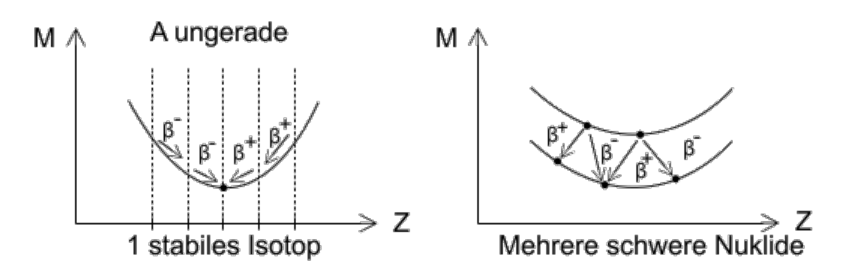
\includegraphics[width=.75\textwidth]{imgs/ep5-fig-5-7.pdf}
\caption{Massenparabel für verschiedene Ausgangsbedingungen\label{fig:5.7}}
\end{figure}

\item \tb{Betazerfall in der Nuklid-Ebene}

\begin{figure}[!ht]
\centering
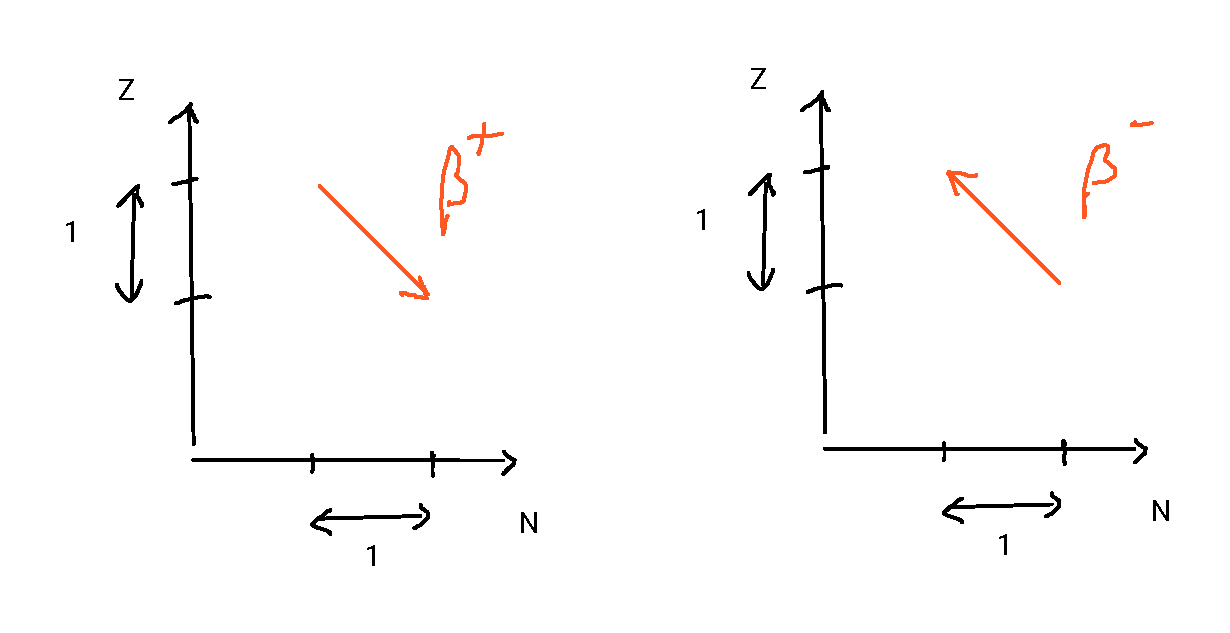
\includegraphics[width=.5\textwidth]{imgs/ep5-fig-5-8.pdf}
\caption{Umwandlung eines Kerns unter $\beta^+$-Zerfall (links) und $\beta^-$-Zerfall (rechts) in der Nuklid-Ebene \label{fig:5.8}}
\end{figure}
\item \tb{$e^{\pm}$-Energiespektrum}\\
Beobachtet: $e^{\pm}$ haben kontinuierliches Energiespektrum
\begin{align*}
0 \leq E_\mr{kin}^e \leq \lno E_\mr{kin}^e\rabs_\mr{max} \approx Q
\end{align*}
\begin{figure}[!ht]
\centering
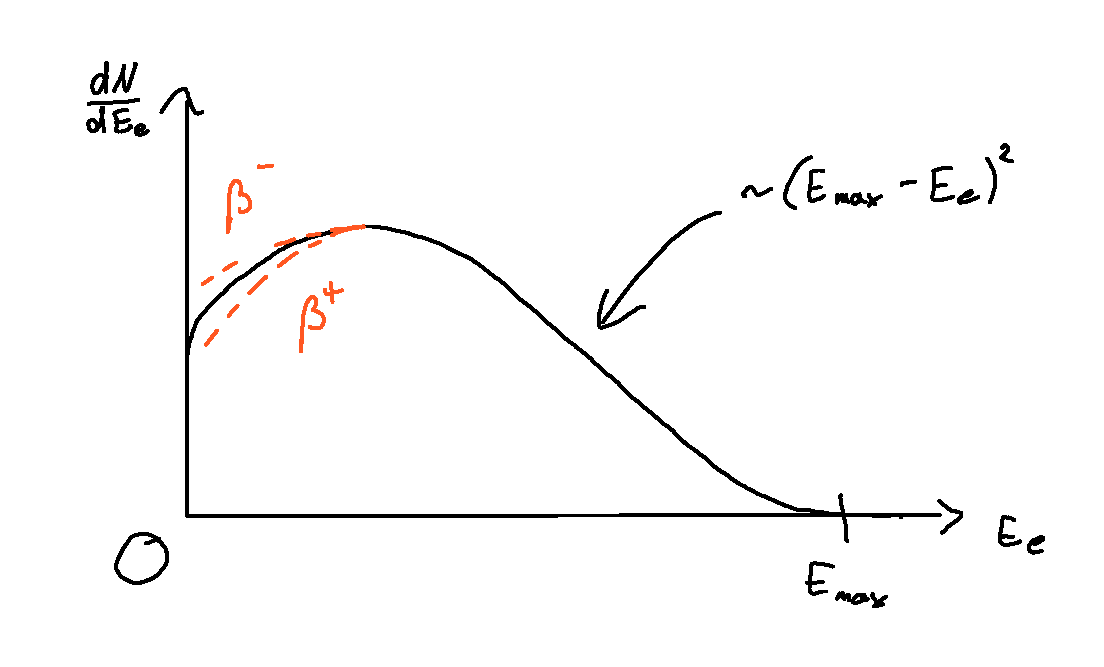
\includegraphics[width=.5\textwidth]{imgs/ep5-fig-5-9.pdf}
\caption{Energiespektrumsgrafik der $e$-Energie\label{fig:5.9}}
\end{figure}
$\leadsto$ 1930: Verletzung von $E$- und $p$-Erhaltung oder neues Teilchen!
\begin{compactitem}
\item[$\Ra$] Pauli postuliert Neutrino
\item[$\Ra$] Nachgewiesen 1956
\end{compactitem}
\item \tb{$\beta$-Zerfall und Neutrinomasse}\\
Wenn $m_\nu > 0$ $\Ra$ $\lno E_\mr{kin}^e\rabs_\mr{max} \approx Q-m_\nu$\\
$\Ra$ Änderung des E-Spektrums bei $\lno E^e_\mr{kin}\rabs_\mr{max}$
\begin{figure}[!ht]
\centering
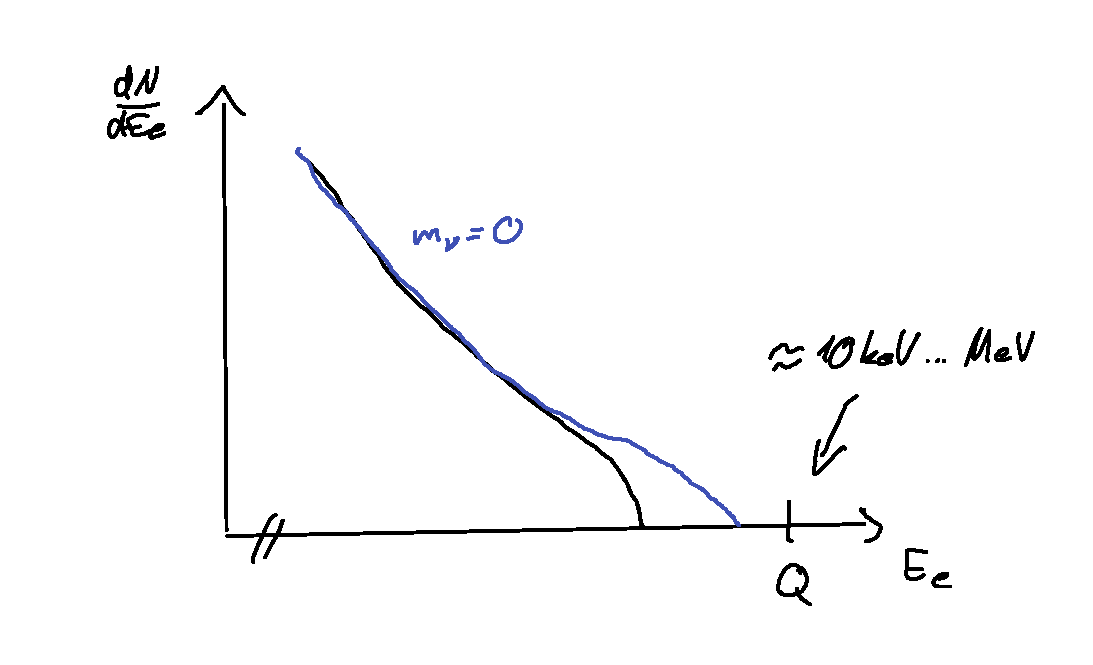
\includegraphics[width=.5\textwidth]{imgs/ep5-fig-5-10.pdf}
\caption{Korrektur (schwarz), wenn Neutrinos massenbehaftet sind\label{fig:5.10}}
\end{figure}

Messung erfordert:
\begin{compactitem}
\item Höchste Messgenauigkeit
\item kleiner $Q$-Wert
\end{compactitem}
Derzeit:
\begin{align}
\boxed{m_\nu < 1.1\,\mr{eV} \text{ mit } 90\,\% C.L.}
\end{align}
aus Tritium-Zerfall
\begin{align*}
^3_1\mr H \underset{Q=18.6\,\mr{keV}}{\ra}\, ^3_2 \mr{He} + e^- + \bar{\nu}_e
\end{align*}
(zukünftig: KATRIN in Karlsruhe: $\sim 0.2\,\mr{eV}$)
\end{itemize}

\section{Doppelbeta-Zerfall}
Falls mehrere stabile Isobare ($\ra$ gg-Kerne):\\
Zerfall durch \glqq 2 simultane Betazerfälle\grqq{} .
\begin{figure}[!ht]
\centering
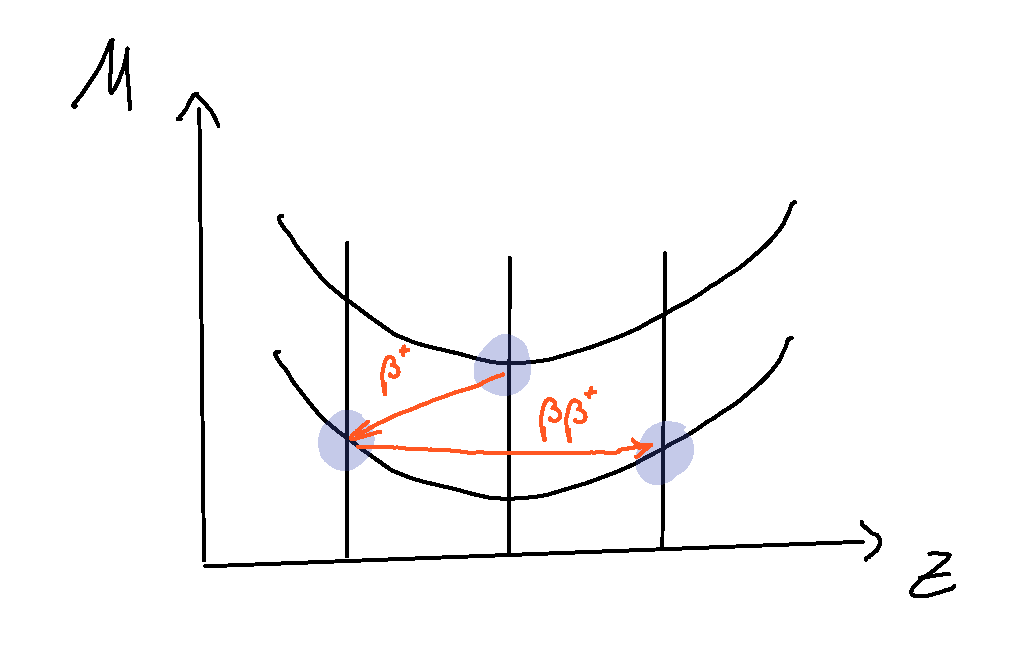
\includegraphics[width=.5\textwidth]{imgs/ep5-fig-5-11.pdf}
\caption{Doppelbeta-Zerfall aufgetragen mit der Masse über die Ordnungszahl\label{fig:5.11}}
\end{figure}
\begin{align}
 ^A_Z X_N \ra ^A_{Z\pm 2} Y_{N\pm 2} + 2e^\pm + 2 \bar{\nu}_e (\text{oder } + 2\nu_e)
\end{align}
\begin{itemize}
\item[$\lt$] Prozess höherer Ordnung (extrem unterdrückt, aber möglich)\\
\begin{figure}[!ht]
    \centering
    \begin{tikzpicture}
        \begin{feynman}
            \vertex (a1) {$u$};
            \vertex[right=6cm of a1] (a2) {$u$};
            \vertex[right=3cm of a1] (a3);
            \vertex[below=2em of a1] (b1) {$d$};
            \vertex[below=2em of a2] (b2) {$d$};
            \vertex[right=3cm of a1] (b3);
            \vertex[below=2em of b1] (d1) {$u$};
            \vertex[right=3cm of d1] (d2);
            \vertex[below=2em of b2] (d3) {$d$};
            \vertex[below=2em of d3] (c1) {$\nu_e$};
            \vertex[below=2em of c1] (c3) {$e^+$};
            \vertex at ($(c1)!0.5!(c3) - (2cm, 0)$) (c2);
            
            \vertex[below=10em of d1] (f1) {$u$};
            \vertex[right=6cm of f1] (f2) {$d$};
            \vertex[right=3cm of f1] (f3);
            \vertex[below=2em of f1] (g1) {$d$};
            \vertex[below=2em of f2] (g2) {$d$};
            \vertex[right=3cm of f1] (g3);
            \vertex[below=2em of g1] (h1) {$u$};
            \vertex[right=3cm of h1] (h2);
            \vertex[below=2em of g2] (h3) {$u$};
            \vertex[above=2em of f2] (i1) {$\nu_e$};
            \vertex[above=2em of i1] (i3) {$e^+$};
            \vertex at ($(i1)!0.5!(i3) - (2cm, 0)$) (i2);

            \diagram* {
            (b1) -- [fermion] (b2),
            (d1) -- [fermion] (d2) -- [fermion] (d3),
            (c3) -- [fermion] (c2) -- [fermion] (c1),
            (d2) -- [scalar, edge label'=$W^+$] (c2),
            (a1) -- [fermion] (a2),
            (g1) -- [fermion] (g2),
            (h1) -- [fermion] (h3),
            (i3) -- [fermion] (i2) -- [fermion] (i1),
            (f3) -- [scalar, edge label=$W^+$] (i2),
            (f1) -- [fermion] (f3) -- [fermion] (f2),
            };
            \draw [decoration={brace}, decorate] (d1.south west) -- (a1.north west)
            node [pos=0.5, left] {$p$};
            \draw [decoration={brace}, decorate] (a2.north east) -- (d3.south east)
            node [pos=0.5, right] {$n$};
            \draw [decoration={brace}, decorate] (h1.south west) -- (f1.north west)
            node [pos=0.5, left] {$p$};
            \draw [decoration={brace}, decorate] (f2.north east) -- (h3.south east)
            node [pos=0.5, right] {$n$};
        \end{feynman}
    \end{tikzpicture}
    \caption{Simultaner $\beta$-Zerfall zweier Protonen \label{fig:5.12}}
\end{figure}
\item[$\lt$] \tb{Beispiel:}
\begin{align}
\begin{split}
^{48}_{20} \mr{Ca} \overset{2\beta^-}{\longrightarrow} ^{48}_{22}\mr{Ti} \qquad \tau = 4\times 10^{19}\,\mr{a}\\
^{76}_{32} \mr{Ge} \overset{2\beta^-}{\longrightarrow} ^{76}_{34}\mr{Se} \qquad \tau = 1.5\times 10^{21}\,\mr{a}
\end{split}
\end{align}
\item \tb{Neutrinoloser Doppelbeta-Zerfall}\\
Hypotetisch, aber höchst interessant
\begin{figure}[!ht]
\centering
    \begin{tikzpicture}
        \begin{feynman}
            \vertex (a1) {$u$};
            \vertex[right=6cm of a1] (a2) {$u$};
            \vertex[right=3cm of a1] (a3);
            \vertex[below=2em of a1] (b1) {$d$};
            \vertex[below=2em of a2] (b2) {$d$};
            \vertex[right=3cm of a1] (b3);
            \vertex[below=2em of b1] (d1) {$u$};
            \vertex[right=3cm of d1] (d2);
            \vertex[below=2em of b2] (d3) {$d$};
            \vertex[below=3em of d3] (c1) {$e^+$};
            \vertex[left=2cm of c1] (c2);
            \vertex[below=8em of d1] (f1) {$u$};
            \vertex[right=6cm of f1] (f2) {$d$};
            \vertex[right=3cm of f1] (f3);
            \vertex[below=2em of f1] (g1) {$d$};
            \vertex[below=2em of f2] (g2) {$d$};
            \vertex[right=3cm of f1] (g3);
            \vertex[below=2em of g1] (h1) {$u$};
            \vertex[right=3cm of h1] (h2);
            \vertex[below=2em of g2] (h3) {$u$};
            \vertex[above=3em of f2] (i1) {$e^+$};
            \vertex[left=2cm of i1] (i2);
            \node[above = .5em of i2, crossed dot] (x1);

            \diagram* {
            (b1) -- [fermion] (b2),
            (d1) -- [fermion] (d2) -- [fermion] (d3),
            (c1) -- [fermion] (c2),
            (d2) -- [scalar, edge label'=$W^+$] (c2),
            (a1) -- [fermion] (a2),
            (g1) -- [fermion] (g2),
            (h1) -- [fermion] (h3),
            (i1) -- [fermion] (i2),
            (f3) -- [scalar, edge label=$W^+$] (i2),
            (f1) -- [fermion] (f3) -- [fermion] (f2),
            (c2) -- (x1),
            (i2) -- (x1),
            };
            \draw [decoration={brace}, decorate] (d1.south west) -- (a1.north west)
            node [pos=0.5, left] {$p$};
            \draw [decoration={brace}, decorate] (a2.north east) -- (d3.south east)
            node [pos=0.5, right] {$n$};
            \draw [decoration={brace}, decorate] (h1.south west) -- (f1.north west)
            node [pos=0.5, left] {$p$};
            \draw [decoration={brace}, decorate] (f2.north east) -- (h3.south east)
            node [pos=0.5, right] {$n$};
        \end{feynman}
    \end{tikzpicture}
\caption{Feynman-Diagramm für neutrinolosen Doppelbeta-Zerfall \label{fig:5.13}}
\end{figure}
\begin{compactitem}
\item[$\lt$] Nur möglich, wenn $\nu = \bar{\nu}$ \glqq Majorana-Neutrinos\grqq{}
\item[$\ra$] Im Standardmodell verboten
\item[$\ra$] Intensive experimentelle Suche, bisher \tb{nicht} gefunden
\begin{compactitem}
\item[$\lt$] $\tau\left(0\nu 2\beta\right) > 10^{25}\,$a
\end{compactitem}
\end{compactitem}
\end{itemize}

\section{Gamma-Strahlung und innere Konversion}
Angeregte Kerne entstehen
\begin{compactitem}
\item als Zerfalls- oder Spaltprodukte
\item durch Beschuss mit $e,\ \gamma, \ p, \ n, \ N,\ \dots$
\end{compactitem}
Zerfall durch $\gamma$-Emission:
\begin{align}
\boxed{\underbrace{^A_Z X^\star_N}_{J_i^P} \ra \underbrace{^A_Z X_N}_{J_f^P} + \underbrace{\gamma}_{J_\gamma^P}} \qquad \mc{O}_\gamma(\mr{MeV})
\end{align}
$J_\gamma^P$ entspricht Drehimpuls $\vec{L}_\gamma$\\
Drehimpuls und Parität erhalten (elm. Prozess) $\Ra$
\begin{align}
\begin{split}
\vec{J}_i = \vec{J}_f + \vec{L}_\gamma \\
P_i = P_f \cdot P_\gamma
\end{split}
\end{align}
Multipolentwicklung: Es gibt elektrische (E) und magnetische (M) Multipolstrahlung
\begin{table}[!ht]
\centering
\begin{tabular}{|c|c|c|c|}
\hline
$L_\gamma$ & E & M & Name\\
\hline
1 & E1 & M1 & Dipol \\
2 & E2 & M2 & Quadrupol\\
3 & E3 & M3 & Oktupol\\
\dots & \dots & \dots & \dots\\
\hline
 & $P_\gamma = (-1)^{L_\gamma}$ & $P_\gamma = (-1)^{L_\gamma +1}$ & \\
 \hline
\end{tabular}
\end{table}

\tb{Auswahlregeln:} 
\begin{align}
\begin{split}
\labs J_i - J_f \rabs \leq L_\gamma \leq J_i + J_f\\
P_\gamma = (-1)^{L_\gamma} \cdot \llb \begin{matrix}
+1 \ (E) \\ -1\ (M) \end{matrix}\rno\qquad \overset{!}{=} \frac{P_i}{P_f}
\end{split}
\end{align}
\tb{Übergangswahrscheinlichkeit:}\\
\glqq klassisches Argument\grqq{}:
\begin{align*}
\labs \vec{L}_\gamma \rabs = L_\gamma \hbar = x \labs \vec{P}_\gamma \rabs = x \frac{E_\gamma}{c}\\
\Ra x = L_\gamma \frac{\hbar c}{E_\gamma} = L_\gamma \frac{197\,\mr{keV\,fm}}{1\,\mr{MeV}}= 200 L_\gamma \cdot \mr{fm} \gg R_k
\end{align*}
$\Ra$ größere $L_\gamma$ stark unterdrückt! QM-Rechnung:
\begin{align}
\boxed{ \lambda \sim E_\gamma (E_\gamma R_k)^{2L_\gamma}\cdot \llb \begin{matrix}
1 \ (E) \\ 0.1 \ (M)\end{matrix} \rno}
\end{align}
$E_\gamma = 1\,\mr{MeV}, \ A = 100$ $\Ra$ $(E_\gamma R_k) \approx 0.03$ $\Ra$ $(E_\gamma R_k)^2 \approx 10^{-3}$
\begin{itemize}
\item[$\Ra$] Niedrigstes erlaubtes $L_\gamma$ dominiert (oder $L_\gamma +1$, wenn $L_\gamma$ M-Übergang, vgl. Tab.\ref{tab:5.1})
\begin{table}[!ht]
\centering
\begin{tabular}{c|c|c|c|c|c}
$\Delta J = \labs J_i - J_f \rabs$ & 0 & 1 & 2 & 3 & \dots \\
\hline
$\frac{P_i}{P_f}$ = +1 & M1, E2 & M1, E2 & E2 & M3, E4 \\
$\frac{P_i}{P_f}$ = -1 & E1 & E1 & M2, E3 & E3 \\
\hline
\end{tabular}
\caption{Verschiedene Multipolstrahlungen verschiedener Werte für $\Delta J$ und $P_\gamma$ \label{tab:5.1}}
\end{table}

\item[$\lt$] $L_\gamma$ nachweisbar über Winkelcharakteristik der Strahlung $Y^l_m\ \dots$
\begin{figure}[!ht]
\centering
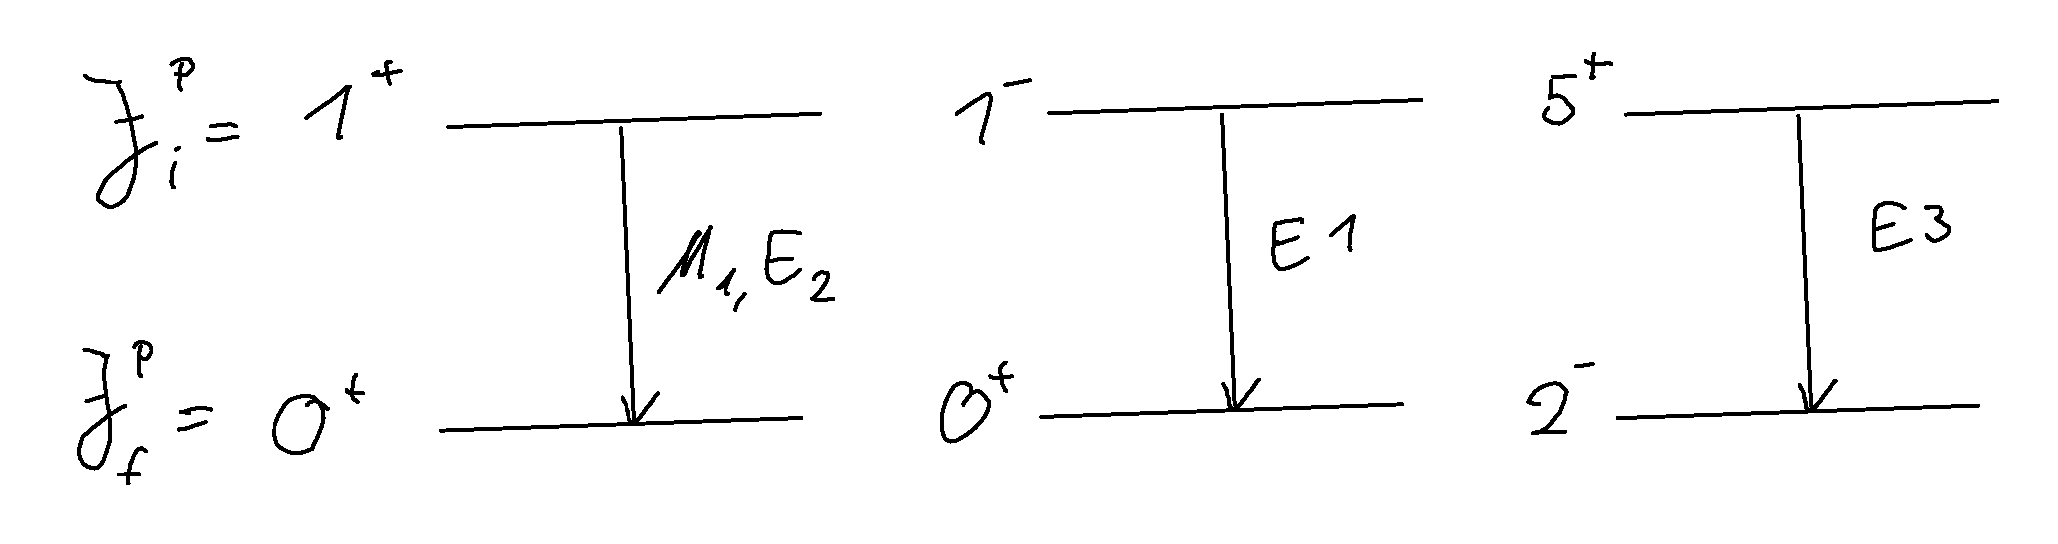
\includegraphics[width=.5\textwidth]{imgs/ep5-fig-5-14.pdf}
\caption{Häufig: Kaskaden über Zwischenzustände\label{fig:5.14}}
\end{figure}\\
\tb{Typische Lebensdauern}\\
$10^{-15} \dots 10^{-9}$\,s\\
Aber: Übergänge mit $\labs \Delta J \rabs \geq 4$ können längerlebig sein, z.B. 
\begin{align*}
^{110}Ag^\star (6^+) \overset{M4}{\ra}\ ^{110}Ag(2^-) + \gamma
\end{align*}
mit $T_{\nicefrac{1}{2}} = 235$\,d (\glqq Isomere\grqq)\\
\tb{Bemerkung:} $6^+$ entspricht $J=6$ und positiver Parität
\item \tb{Innere Konversion}\\
Alternativ zu $\gamma$-Emission
\begin{align}
\boxed{\left( ^A_Z X^\star_N \right)^0 \ra \left( ^A_Z X_N \right)^+ + e^-}
\end{align}
nachfolgend Röntgenstrahlung oder Auger-Elektron
\end{itemize}


\section{Kernspaltung}
Aufbrechen eines Kerns in zwei Tochterkerne und Neutronen:
\begin{align*}
\boxed{^A_ZX_N \ra ^{A_1}_{Z_1}{Y_1}_{N_1} + ^{A_2}_{Z_2}{Y_2}_{N_2} + kn}\\
A = A_1 + A_2 + k; \ Z = Z_1 + Z_2; \ N = N_1 + N_2 +k
\end{align*}
$Q$-Wert $>$ 0 für schwere Kerne, aber: Coulomb-Barriere\\
Kernspaltung kann (in Bezugnahme zum Tröpfchenmodell) beschrieben werden als Verformung:

\begin{figure}[!ht]
	\centering
	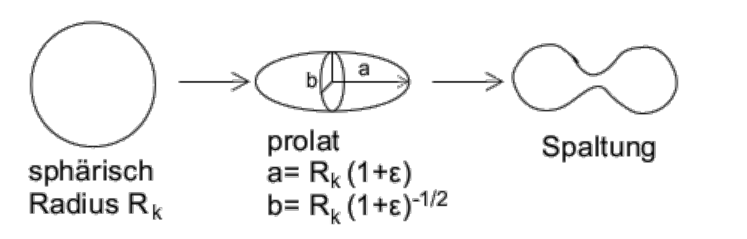
\includegraphics[width=.6\textwidth]{imgs/ep5-fig-5-15.pdf}
	\caption{Verzerrung des \glqq Nukleonentropfens\grqq{} bis hin zur Spaltung in zwei neue \glqq Tropfen\grqq \label{fig:5.15}}
	\end{figure}

\begin{figure}[!ht]
	\centering
	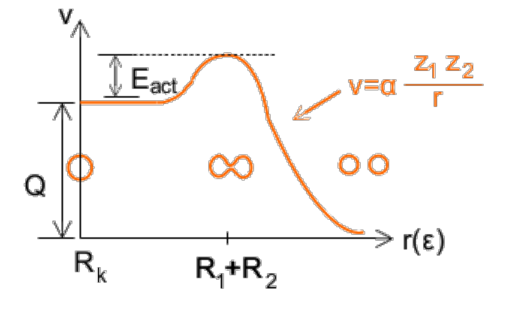
\includegraphics[width=.5\textwidth]{imgs/ep5-fig-5-16.pdf}
	\caption{Schematische Skizze zur Aktivierungsenergie $E_\mr{act}$, die für eine Kernspaltug nötig ist \label{fig:5.16}}
\end{figure}

\tb{3 Fälle:}
\begin{itemize}
\item[(i)] $E_\mr{act} < 0$ $\Ra$ Kern nicht gebunden
\item[(ii)] $E_\mr{act} > 0$, aber klein\\\
$\Ra$ Spontane Spaltung durch Tunnelprozess (ähnlich $\alpha$-Zerfall)
\item[(iii)] $E_\mr{act} > 0$ und groß\\
$\Ra$ Spaltung erfordert Energiezufuhr
\end{itemize}
\tb{Im Tröpfchenmodell:}
$E_s$, $E_c$ hängen von $\epsi$ ab.
\begin{align*}
\lno \begin{matrix}
E_s (\epsi) = a_s A^{\nicefrac{2}{3}} \left( 1+ \frac{2}{5}\epsi^2 + \dots \right) \\ E_c(\epsi) = \underbrace{a_c Z^2 A^{-\nicefrac{1}{3}}}_\text{Weizsäcker-Formel} \left( 1 - \frac{1}{5} \epsi^2 + \dots \right)
\end{matrix} \rrb \text{ohne Rechnung (Taylorentwicklung)}\\
\Ra \Delta E (\epsi) =\lno M(A,Z) \rabs_\epsi - \lno M(A,Z) \rabs_{\epsi=0} = \frac{\epsi^2}{5} \left( 2 a_s A^{\nicefrac{2}{3}} - a_c Z^2 A^{-\nicefrac{1}{3}}\right)
\end{align*}
\begin{itemize}
\item[$\Ra$] \tb{Fall (i)}, wenn $\Delta E (\epsi) < 0$
\begin{align}
\lt \ \boxed{\frac{Z^2}{A} > \frac{2 a_s}{a_c} \approx 48}
\end{align}
\begin{itemize}
\item[$\lt$] erfüllt für $Z \geq 114$, $A \gtrsim 290$
\item[$\lt$] Solche Kerne sind nicht gebunden $\ra$ nicht existent
\end{itemize}
\tb{Fall (ii): Spontane Spaltung}
\begin{align}
\begin{matrix}
 & \nearrow & ^{234}_{90}\mr{Th} & \left(\sim 100 \%\right) \qquad \text{Zerfall}\\
^{238}_{92} \mr U & & & \\
 & \searrow & \dots & \left(5\cdot 10^{-5}\%\right) \qquad \text{Spaltung}
\end{matrix}
\end{align}
\tb{Fall (iii): Induzierte Spaltung}\\
Insbesondere durch Beschuss mit Neutronen.\\
Beispiel:
\begin{align*}
^{238}_{92} \mr U + n \ra ^{239}_{92} \mr U + E_\mr{exc}
\end{align*}
Energiebilanz:
\begin{align}
\boxed{E_\mr{exc} = \underbrace{M(A,Z) + M_n - M(A+1, Z)}_{\Delta M (A,Z)} + T_n}\\
 T_n \ = \ \text{kin. Energie des Neutrons}\nonumber
\end{align}
Spaltung, falls $E_\mr{exc} > E_\mr{act}$\\
$\Ra$ 2 Fälle
\begin{itemize}
\item[(i)] $\Delta M (A,Z) > E_\mr{act}$: $T_n$ wird \glqq nicht benötigt\grqq{}, Spaltung durch langsame Neutronen\\
z.B. $^{235}_{92}\mr U$, $^{233}_{90}\mr{Th}$, $^{239}_{94} \mr{Pu}$
\begin{compactitem}
\item[$\lt$] Kettenreaktion
\item[$\lt$] gu-Kern + n $\ra$ gg-Kern
\end{compactitem}
\item[(ii)] $\Delta M(A,Z) < E_\mr{act}$ $\Ra$ $T_n \geq E_\mr{act} - \Delta M(A,Z)$\\
$\Ra$ Spaltung durch schnelle Neutronen. Z.B.:
\begin{align*}
^{238}_{92}\mr U \ \left( T_n \gtrsim 0.6\,\mr{MeV}\right)
\end{align*}
\end{itemize}
\tb{WQ für n-Einfang} (vgl. Kap.\ref{chap:3})
\begin{align}
\boxed{\sigma_n \sim \frac{1}{j_n} \sim \frac{1}{v_n} \sim \frac{1}{\sqrt{T_n}}}
\end{align}
$\Ra$ n-Einfang \tb{viel} effizienter für thermische als für schnelle Neutronen
\end{itemize}
\section{Das Prinzip von Kernreaktoren}
Kettenreaktion durch n-Einfang
\begin{align*}
^{235}_{92}U + n \ra X + Y + \lla 2.5 n\rra
\end{align*}
\tb{Multiplikationsfaktor}
\begin{align*}
\boxed{k = \frac{\# \text{sekundäre Spaltungen}}{\text{Primärspaltung}}}
\end{align*}
$k<1$: keine Kettenreaktionen (subkritisch)\\
$k=1$: stabile Kettenreaktion (kritisch) $\ra$ KKW\\
$k>1$: exponentielles Wachstum (superkritisch) $\ra$ Kernwaffen\\
Ein Reator muss also auf $k=1$ geregelt werden. Dies erfordert:
\begin{compactitem}
\item[$\ra$] Angereichertes $^{235}_{92}U$
\item[$\ra$] Abbremsen der n
\begin{compactitem}
\item[$\ra$] Stöße mit leichten Kernen (z.B.: $H_2O$, $D_2O$, $C$), genannt \glqq Moderator\grqq{}
\item[$\ra$] Ziel: $\frac{\Pa k}{\Pa T} < 0$
\begin{compactitem}
\item[$\lt$] Stabilisierend, z.B. für $H_2O$, $D_2O$
\end{compactitem}
\end{compactitem}
\item[$\ra$] Regelung der n-Dichte
\begin{compactitem}
\item[$\ra$] n-Absorber (z.b. $Cd$), genannt \glqq Kontrollstäbe\grqq{}
\end{compactitem}
\end{compactitem}
\begin{figure}[!ht]
\centering
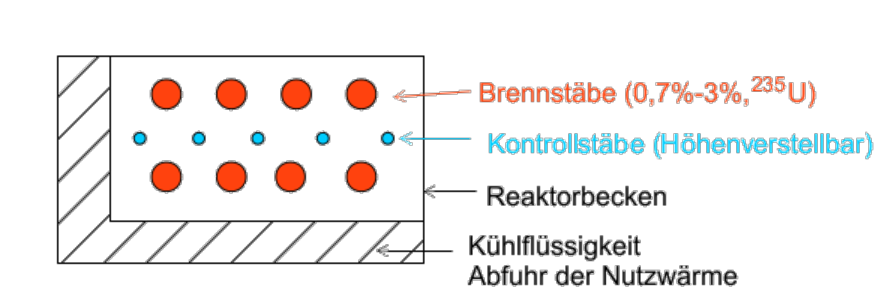
\includegraphics[width=.6\textwidth]{imgs/ep5-fig-5-17.pdf}
\caption{Schematischer Aufbau eines Reaktorbeckens \label{fig:5.17}}
\end{figure}
Nach Abschaltung:
\begin{compactitem}
\item keine Kettenreaktion
\item Aber \glqq Nachzerfallswärme\grqq{} durch radioaktive Zerfälle und Restneutronen
\item[$\ra$] unkontrollierter Anstieg der Temperatur, wenn das Kühlsystem versagt (\glqq Kernschmelze\grqq{}, z.B. Tschernobyl und Fukushima)
\end{compactitem}

\chapter{Die Struktur des Nukleons}
Nukleon ist ausgedehntes Objekt.\\
Radius $\sim \mc{O}(\mr{fm})$. Untersuchung in Lepton-Nukleon-Streuung:
\begin{align*}
ep, \ \mu p , \ \nu(\bar{\nu}) p, eA, \mu A, \nu(\bar{\nu}) A
\end{align*}
Im Folgenden wird die Elektron-Proton-Streuung betrachtet.

Energieskala: $\Delta p \, \Delta x > \hbar \ \Ra \ E \gtrsim 1$\,GeV mit $\Delta p = \labs \vec{q}\rabs$ und $\Delta x = R_N < 1$\,fm\\
Typisch für $E$ sind $1 \dots 400$\,GeV

Bei HERA (DESY, Hamburg) ep-Kollisionen. Entspr. 50\,TeV Strahlenenergie in Fixed-Target-Experiment

\section{eN-Streuung -- Kinematik und WQ}
hier: QM (statt QFT nötig $\Ra$ Näherungen), Schrödingergleichung (obwohl relativistische Kinematik)

\begin{itemize}
\item \tb{Kinematik}\\
\begin{figure}[!ht]\centering
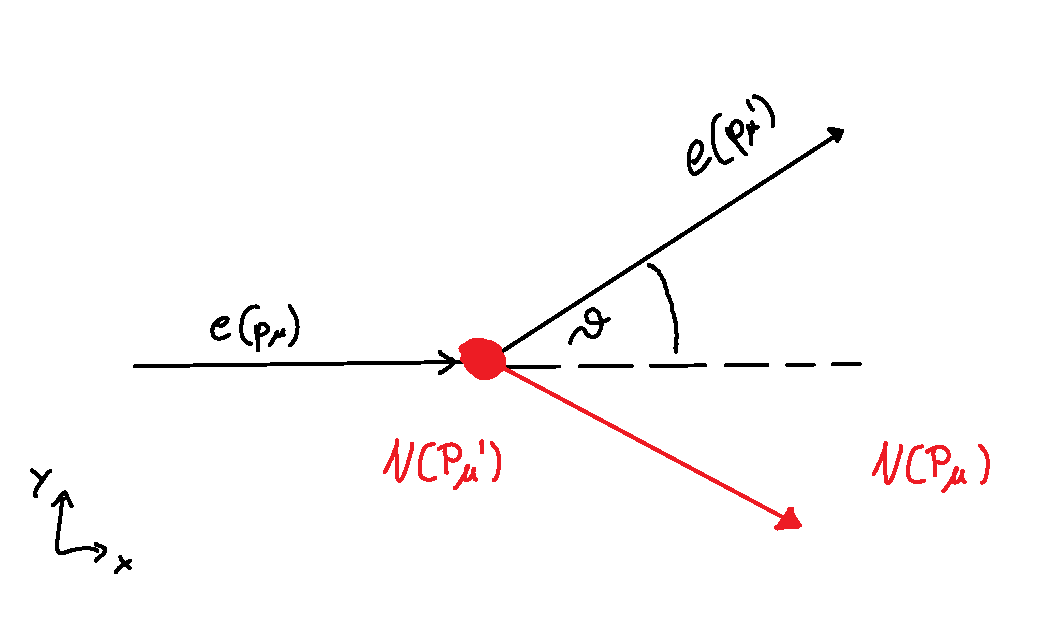
\includegraphics[width=.6\textwidth]{imgs/ep5-fig-6-1.pdf}
\caption{Elektron-Nukleon-Streuung \label{fig:6.1}}
\end{figure}
\begin{align}
\begin{split}
p_\mu = (E,p,0,0)\\
p_\mu^\prime = \lb E^\prime, p^\prime \cos \vartheta,  p^\prime \sin \vartheta,0 \rb \\
P_\mu = (M,0,0,0)
\end{split}
\end{align}
$E$- und $p$-Erhaltung:
\begin{align}
\begin{split}
\lb  p_\mu + P_\mu\rb ^2 = \lb p_\mu^\prime + P_\mu^\prime\rb ^2\\
\Ra \underbrace{p_\mu^2 + P_\mu^2 }_{m^2+M^2} + 2p_\mu P^\mu = \underbrace{{p_\mu^\prime}^2 + {P_\mu^\prime}^2}_{m^2+M^2} + 2p_\mu^\prime P^{\mu\prime}\
\Ra p_\mu P^\mu = p_\mu^\prime \lb  p^\mu + P^\mu - p^{\mu\prime}\rb \\
\Ra EM = \underbrace{p_\mu^\prime p^\mu}_{EE^\prime - pp^\prime \cos \vartheta} + E^\prime M - m^2
\end{split}
\end{align}
\begin{align}
\begin{split}
\boxed{E^\prime = E - \underbrace{\frac{EE^\prime - pp^\prime \cos \vartheta - m^2}{M}}_{>0, \text{ klein wenn } M\gg E}}
\end{split}
\end{align}
\begin{enumerate}
\item Wenn $M\gg E$ $\Ra$ $E^\prime = E$ (Rutherford, eN bei $E\sim 10$\,MeV)
\item Wenn $m\ll E$ $\Ra$ $E=p,\ E^\prime = p^\prime$
\begin{align}
\begin{split}
\Ra \boxed{E^\prime = \frac{E}{1 + \frac{E}{M}\lb  1- \cos \vartheta\rb }}
\end{split}
\end{align}
(eN-Streuung bei $E \gtrsim 10$\,MeV)
\end{enumerate}
\item \tb{Potentialstreuung}\\
Fall (1): $M \gg E$, \glqq kein\grqq{} E-Übertrag auf N
\begin{itemize}
\item[$\Ra$] Wie Streuung in ortsfestem Potential $V\lb \vec{r}\rb $ \\$\ra$ Hamiltonian $\Ham\lb \vec{r}\rb $
\begin{figure}[!ht]
\centering
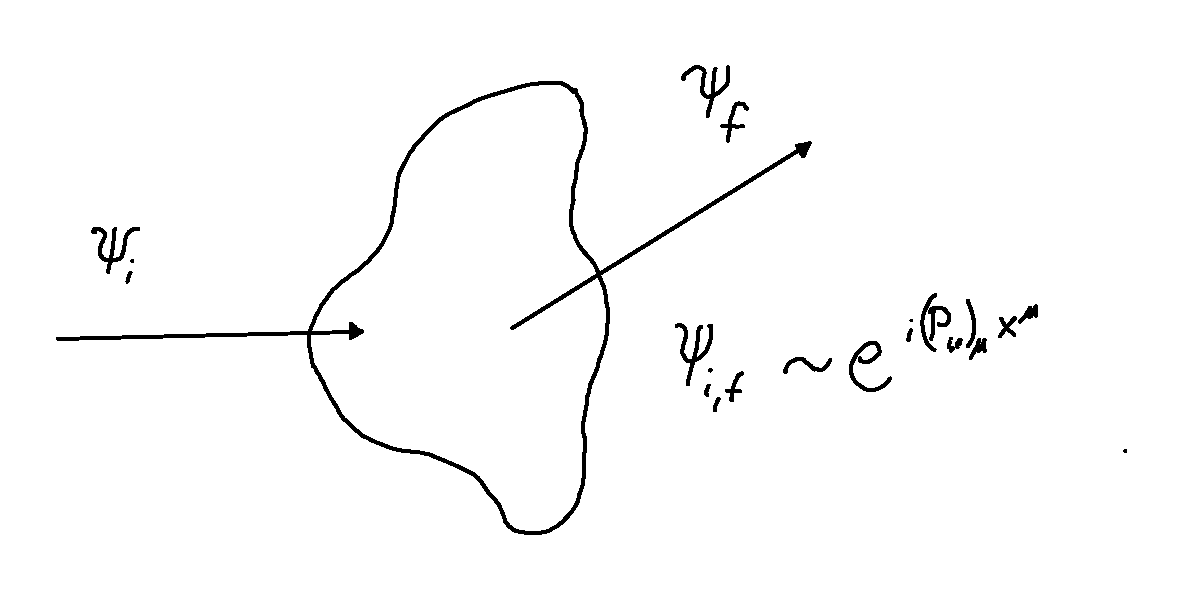
\includegraphics[width=.6\textwidth]{imgs/ep5-fig-6-2.pdf}
\caption{Veranschaulichung des Hamiltonian als WW-Operator\label{fig:6.2}}
\end{figure}
\item[$\Ra$] Nutze: \begin{compactitem}
\item QM-Störungsrechnung
\item Fermis Goldene Regel
\item Zustandsdichte im Endzustand
\end{compactitem}
\begin{align}
\Ra \boxed{ \Pa \sigma = \frac{{E^\prime}^2}{\lb  2\pi\rb ^2} \labs \int \Pa^3 r e^{i \vec{q}\vec{r}} \Ham\lb \vec{r}\rb  \rabs^2 \Pa \Omega }
\end{align}
\begin{compactitem}
\item[mit] $\vec{q} = \vec{p}-\vec{p}^\prime$
\item[] $\Ham\lb \vec{r}\rb  = (-e) V_A\lb \vec{r}\rb $
 \item[] $V_A$ als Coulombpotential des Targets
\end{compactitem}
$V_A\lb \vec{r}\rb $ wird von Ladungsdichte $\rho_A\lb \vec{r}\rb $ erzeugt\\
$\rho_A\lb \vec{r}\rb  = e f_A\lb \vec{r}\rb $ mit $\int \Pa^3 r f_A\lb \vec{r}\rb  = 1$\\
Somit die Poissongleichung (Elektrostatik)
\begin{align}
\boxed{\Lap V_A\lb \vec{r}\rb  = - \frac{\rho_A\lb \vec{r}\rb }{\epso} = -\frac{e}{\epso}f_A\lb \vec{r}\rb }
\end{align}
\begin{align*}
& \Ra \int \Pa^3 r e^{i \vec{q}\vec{r}} \Ham \lb \vec{r}\rb \\
&\qquad \labs\ \Lap e^{i \vec{q}\vec{r}} = - \labs \vec{q}\rabs^2 e^{i \vec{q}\vec{r}} \rno\\
& =  - \int \Pa^3 r \frac{1}{\labs\vec{q}\rabs^2} \lb  \Lap e^{i \vec{q}\vec{r}}\rb  \Ham\lb \vec{r}\rb \\
&\qquad \labs\ \text{2-fache partielle Integration} \rno \\
& = -\frac{1}{\labs \vec{q}\rabs ^2} \int \Pa^3 r e^{i\vec{q}\vec{r}} \underbrace{\lb  \Lap \Ham \lb \vec{r}\rb \rb }_{-e \frac{-\rho_A \lb \vec{r}\rb }{\epso}}\\
& = - \underbrace{\frac{e^2}{\labs \vec{q}\rabs^2 \epso}}_{=\frac{4\pi\alpha}{\labs \vec{q}\rabs^2}} \underbrace{\int \Pa^3 r e^{i\vec{q}\vec{r}} f_A\lb \vec{r}\rb }_\text{= Formfaktor $F\lb \vec{q}\rb $}
\end{align*}
Für punktförmiges Target:
\begin{align}
f_A \lb  \vec{r}\rb  = \delta \lb  \vec{r}\rb  \ \Ra \ F\lb \vec{q}\rb  \equiv 1,
\end{align}
also
\begin{align}
\boxed{ \begin{matrix}
\frac{\Pa \sigma}{\Pa \Omega} & = \frac{{E^\prime}^2}{\lb 2\pi\rb ^2} \labs \int \Pa^3 r e^{i\vec{q}\vec{r}}\Ham\lb \vec{r}\rb  \rabs^2\\
& = \frac{4 \alpha^2}{\labs \vec{q}\rabs^4}{E^\prime}^2 = \lno \frac{\Pa \sigma}{\Pa \Omega}\rabs_\text{Rutherford}
\end{matrix} }
\end{align}
Hierbei eigentlich: Faktor $Z_e^2 Z_p^2$

Erinnerung:
\begin{align}
\labs \vec{q}\rabs ^2 = \labs \vec{p} - \vec{p}^\prime \rabs^2 \overset{p= p^\prime}{=} 2 p^2 - 2p^2 \cos \vartheta = 4 p^2 \sin^2 \frac{\vartheta}{2}\nonumber \\
p^2 \llb \begin{matrix}
E_{kin} \cdot 2m & \text{nicht-relativistisch (Rutherford)}\\ EE^\prime & \text{relativistisch } (E \approx E^\prime = p)
\end{matrix} \rno \nonumber\\
\Ra \boxed{ \lno \frac{\Pa \sigma^\mathrm{eN}}{\Pa \Omega}\rabs _\mathrm{Rf} = \frac{Z_e^2 Z_p^2 \alpha^2 }{4 E^2 \sin^4 \frac{\vartheta}{2}} }
\end{align}
\end{itemize}
\item \tb{Korrekturen}
\begin{itemize}
\item[$\ra$] Ausgedehntes Target:
\begin{align}
\frac{\Pa \sigma}{\Pa \Omega} = \lno \frac{\Pa \sigma}{\Pa \Omega}\rabs_\mathrm{Rf} \cdot \labs F\lb  \vec{q} \rb  \rabs ^2
\end{align}
\item[$\ra$] Rückstoß-Korrektur (Energieübertrag)
\begin{align}
\frac{\Pa \sigma}{\Pa \Omega} = \lno \frac{\Pa \sigma}{\Pa \Omega}\rabs_\text{Rf} \frac{E^\prime}{E}
\end{align}
\item[$\ra$] Magnetisches Moment des $e^-$ (ohne magn. Moment des $N$)
\begin{align}
\frac{\Pa \sigma}{\Pa \Omega} = \lno \frac{\Pa \sigma}{\Pa \Omega}\rabs_\text{Rf} \cdot \lb  1 - \beta_e^2 \sin^2 \frac{\vartheta}{2}\rb 
\end{align}
für $\beta_e \ \ra \ 1$ (relativistisches $e^-$):
\begin{align*}
1-\beta_e^2 \sin^2\frac{\vartheta}{2} \ \ra \ \cos^2 \frac{\vartheta}{2}
\end{align*}
\item[$\Ra$] Rückstreuung ($\vartheta = 180^\circ$) unterdrückt\\
Grund: Helizitätserhaltung (folgt aus relativistischer QM für $\beta_e \ra 1$)
\begin{align*}
\text{Helizität} =  \frac{\vec \sigma \vec{p}}{\labs \vec{\sigma}\rabs \labs \vec{p} \rabs}
\end{align*}
\begin{align}
\boxed{ \frac{\Pa \sigma}{\Pa \Omega} = \frac{Z_e^2 Z_p^2 \alpha^2 }{4 E^2 \sin^4 \frac{\vartheta}{2}} \frac{E^\prime}{E} \cdot \cos^2 \frac{\vartheta}{2} = \lno \frac{\Pa \sigma}{\Pa \Omega}\rabs_\mathrm{Mott} }\\
\text{zusätzlich } \labs F\lb \vec{q}\rb  \rabs^2
\end{align}
\item[$\ra$] Magnetisches Moment des Targets (punktförmiges Dirac-Teilchen)
\begin{align}
\boxed{ \frac{\Pa \sigma}{\Pa \Omega} \ra \lno \frac{\Pa \sigma}{\Pa \Omega}\rabs_\mathrm{Mott}  \lb  1 + 2 \tau \tan^2 \frac{\vartheta}{2}\rb  }
\end{align}
\begin{compactitem}
\item[mit] $\tau = \frac{Q^2}{4 M^2} = \frac{- q_\mu q^\mu}{4 M^2}$
\end{compactitem}
Jetzt: Spin-Flip von Target möglich, $\lno \nicefrac{\Pa \sigma}{\Pa \Omega} \rabs_{\vartheta = 180^\circ} > 0$
\end{itemize}
\end{itemize}

\section{Elastische eN-Streuung}
N ist \tb{nicht} punktförmig $\Ra$ Formfaktor\\
\tb{2} Formfaktoren
\begin{compactitem}
\item $G_E\lb q^2\rb  \ra $ Verteilung der Ladung
\item $G_M\lb q^2\rb  \ra $ Verteilung der magnetischen Momente
\end{compactitem}
\begin{itemize}
\item[$\Ra$] WQ ist (nach Rosenbluth-Formel)
\begin{align}
\boxed{ \frac{\Pa \sigma}{\Pa \Omega} = \lno \frac{\Pa \sigma}{\Pa \Omega} \rabs_\mr{Mott} \lsb  \frac{G_E^2 +\tau \cdot G_M^2}{1 + \tau} + 2 \tau G_M^2 \tan^2 \frac{\vartheta}{2} \rsb  }
\end{align}
\item[$\ra$] Messung von $\frac{\Pa \sigma}{\Pa \Omega}\lb q^2\rb $ ergibt $G_{E,M}$
\begin{align}
\boxed{
G_{E,M}^p \lb Q^2\rb  = \frac{G_{E,M}^p \lb 0\rb }{\lb  1+ \frac{Q^2}{0.71\,\mr{GeV}^2}\rb ^2}
}
\end{align}

Auch:
\begin{align}
G_M^n = \frac{G_M^n \lb  0\rb }{\lb 1+ \frac{Q^2}{0.71\,\mr{GeV}^2}\rb ^2}
\end{align}
\item[$\Ra$] Ladungsverteilung
\begin{figure}[!ht]
\centering
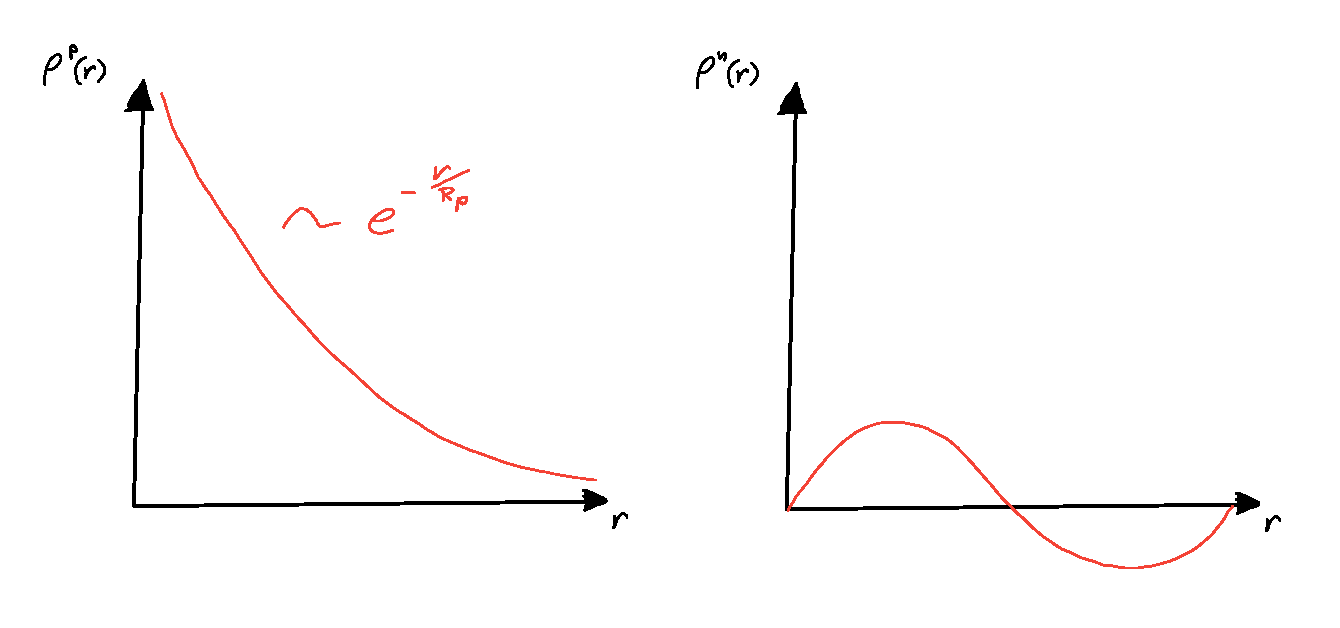
\includegraphics[width=.5\textwidth]{imgs/ep5-fig-6-3.pdf}
\caption{Ladungsverteilung eines Protons\label{fig:6.3}}
\end{figure}

Es gilt hierbei: $R_p \approx 0.86$\,fm
\item[$\ra$] $G_{M,E} \lb  Q^2 = 0\rb $ ist Ladung bzw. magnetisches Moment des Nukleons
\begin{align*}
\begin{matrix}
G_E^p(0) = 1 & \text{Ladung 1}e\\
G_E^n(0) = 0 & \text{Ladung 0}e\\
G_M^p(0) = 2.79 & \text{magnetisches Moment }\mu_p= 2.79\frac{e\hbar}{2M_p}\\
G_M^n(0) = -1.91 & \mu_n = - 1.91\frac{e\hbar}{2M_n}
\end{matrix}
\end{align*}
\end{itemize}

\section{Anregungszustände der Nukleonen}
Inelastische Streuung:
\begin{figure}[!ht]
\centering
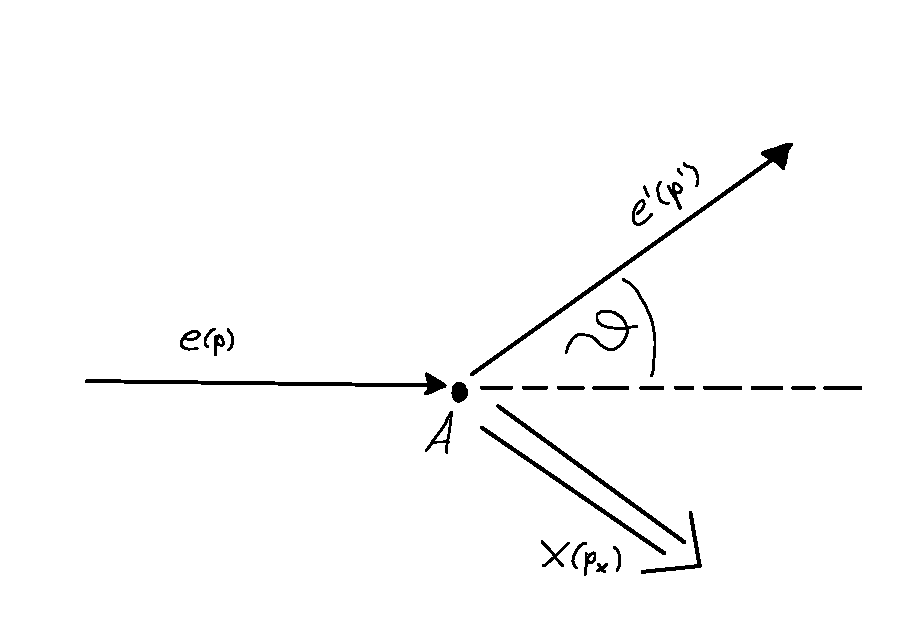
\includegraphics[width=.6\textwidth]{imgs/ep5-fig-6-4.pdf}
\caption{Skizze zur inelastischen Streuung eines $e^-$ an einem Teilchen A\label{fig:6.4}}
\end{figure}
Aus \autoref{fig:6.4}
\begin{align*}
q_\mu = p_\mu - p_\mu^\prime\\
p_{X,\mu} = p_{A,\mu} + q_\mu
\end{align*}
Es gilt also somit:
\begin{align}
\begin{split}
\underbrace{p_X^2}_{W^2} = \underbrace{p_A^2}_{M_A^2} + \underbrace{q_\mu q^\mu}_{-Q^2} + \underbrace{2 p_{A,\mu}q^\mu}_{2M_A\lb E-E^\prime\rb =2 M\nu}\\
\Ra W^2 = -Q^2 + M^2 + 2 \nu M = Q^2 \lsb  \frac{2 \nu M}{Q^2} -1 \rsb  +M^2\\
\frac{2\nu M}{Q^2} = \frac{1}{x}
\end{split}
\end{align}
$x$ = \glqq Bjorken-x\grqq
\begin{itemize}
\item[$\lt$] elastisch: $W^2 = M^2 \Ra x=1$
\item[$\lt$] inelastisch: $W^2 > M^2 \Ra x<1$
\item[$\lt$] $\boxed{2}$ Variablen erforderlich, um inelastische Kinematik festzulegen\\
$\lt$ $\lb x, Q^2\rb $, $\lb x, W\rb $, $\lb E^\prime, \vartheta\rb $
\item[$\Ra$] Messung von $\dfrac{\sigma}{W}$

\begin{figure}[!ht]
\centering
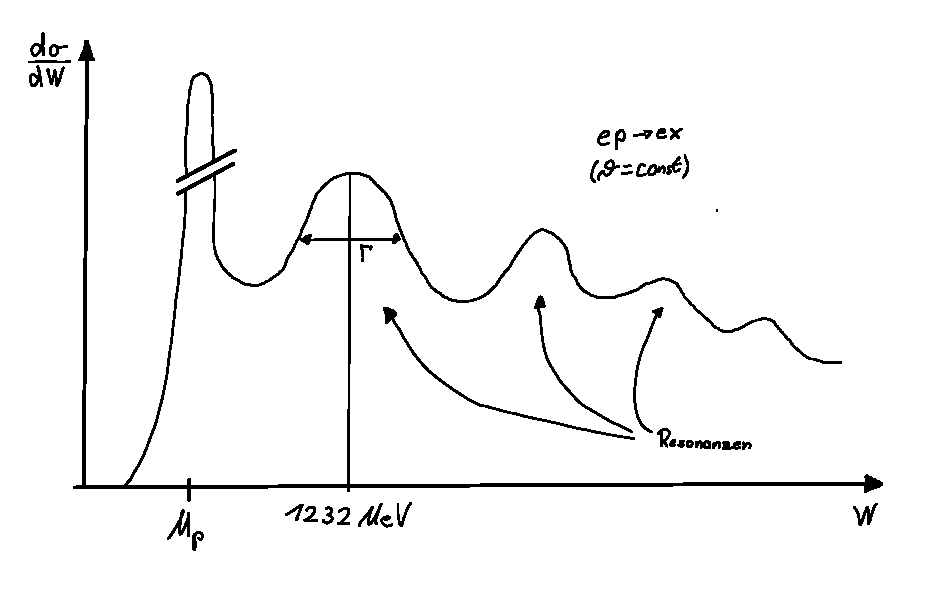
\includegraphics[width=.6\textwidth]{imgs/ep5-fig-6-5.pdf}
\caption{Resonanzpeaks der $eN$-Streuung\label{fig:6.5}}
\end{figure}

\item[$\ra$] Peaks = \glqq Resonanzen\grqq{}
\begin{compactitem}
\item[$\Ra$] kurzlebige Zustände
\item[$\Ra$] Nukleonanregungen
\item[$\Ra$] Prominent: $\Delta^+\lb 1232\rb $
\begin{align}
\begin{split}
M\lb \Delta^+\lb 1232\rb \rb  = 1.232\,\mr{GeV}\\
\Gamma_{\Delta^+} \approx 120\,\mr{MeV}
\end{split}
\end{align}
$\ra$ Lebensdauer des $\Delta^+\lb 1232\rb $:
\begin{align}
\tau = \frac{1}{\Gamma}= \frac{197\,\mr{\nicefrac{MeV}{fm}}}{120\,\mr{MeV}}\frac{1}{c} \approx 0.5\cdot 10^{-23} \,\mr s
\end{align}
$\tau$ ist typischer Wert für starke Wechselwirkung
\end{compactitem}
\item[$\lt$] Genauere Untersuchung:
\begin{align*}
\ket{\Delta^+\lb 1232\rb } = \ket{uud} \ \ \ \text{wie $p$}\\
J^p\lb \Delta^+\lb 1232\rb \rb  = \lb  \frac{3}{2}\rb ^+; \ \ \ J^p \lb p\rb  = \lb  \frac{1}{2}\rb  ^+
\end{align*}
\item[$\lt$] $\Delta$-Zerfall
\begin{figure}[!ht]
\centering
    \begin{tikzpicture}
        \begin{feynman}
            \vertex (a1) {$u$};
            \vertex[right=2cm of a1] (a2);
            \vertex[right=3cm of a1] (a3);
            \vertex[right=5cm of a1] (a4) {$u$};
            \vertex[below=2em of a1] (b1) {$u$};
            \vertex[right=2.5cm of b1] (b2);
            \vertex[right=5cm of b1] (b3) {$u$};
            \vertex[below=2em of b1] (c1) {$d$};
            \vertex[right=5cm of c1] (c2) {$d$};
            \vertex[above=2.667em of a4] (d1) {$\bar u$};
            \vertex[above=4em of a4] (e1) {$u$};
            
            \vertex[right=8cm of a1] (f1) {$u$};
            \vertex[right=2cm of f1] (f2);
            \vertex[right=3cm of f1] (f3);
            \vertex[right=5cm of f1] (f4) {$d$};
            \vertex[below=2em of f1] (g1) {$u$};
            \vertex[right=2.5cm of g1] (g2);
            \vertex[right=5cm of g1] (g3) {$u$};
            \vertex[below=2em of g1] (h1) {$d$};
            \vertex[right=5cm of h1] (h2) {$d$};
            \vertex[above=2.667em of f4] (i1) {$\bar d$};
            \vertex[above=4em of f4] (j1) {$u$};

            \diagram* {
            (a1) -- (a2) -- (e1),
            (a2) -- [gluon] (a3) -- (d1),
            (b1) -- (b3),
            (a3) -- (a4),
            (c1) -- (c2),
            
            (f1) -- (f2) -- (j1),
            (f2) -- [gluon] (f3) -- (i1),
            (g1) -- (g3),
            (f3) -- (f4),
            (h1) -- (h2),
            };
            \draw [decoration={brace}, decorate] (c1.south west) -- (a1.north west)
            node [pos=0.5, left] {$\Delta^+$};
            \draw [decoration={brace}, decorate] (a4.north east) -- (c2.south east)
            node [pos=0.5, right] {$p$};
            \draw [decoration={brace}, decorate] (e1.north east) -- (d1.south east)
            node [pos=0.5, right] {$\pi^0$};

            \draw [decoration={brace}, decorate] (h1.south west) -- (f1.north west)
            node [pos=0.5, left] {$\Delta^+$};
            \draw [decoration={brace}, decorate] (f4.north east) -- (h2.south east)
            node [pos=0.5, right] {$n$};
            \draw [decoration={brace}, decorate] (j1.north east) -- (i1.south east)
            node [pos=0.5, right] {$\pi^+$};
        \end{feynman}
    \end{tikzpicture}
\caption{Zerfallsgrafiken für $\Delta^+$ zu p bzw. n}
\end{figure}
\end{itemize}

\section{Tiefinelastische Streuung}
Frage: Was passiert bei höheren Energien?\\
Erwartung: Bessere räumliche Auflösung $\Ra$ Bestandteile des Nukleons
\begin{itemize}
\item Beobachtung 1\\
Bei $W \gtrsim 2.5$\,GeV: Kontinuum von hadronischen Endzuständen
\begin{itemize}
\item[$\lt$] keine Resonanzen
\item[$\lt$] unterschiedliche Hadronenkombinationen
\item[$\lt$] Differentieller WQ hängt von zwei Variablen ab, z.B.
\begin{align*}
\underbrace{Q^2 = - q_\mu q^\mu; \ \ \ x = \frac{Q^2}{2M\nu} = \frac{- q_\mu q^\mu}{2 P_{A,\mu}q^\mu}}_\text{Lorentz-Invariant}
\end{align*}
\item[$\lt$] Darstellung des WQ:
\begin{align}
\dfrac{^2 \sigma}{\Omega \Pa E^\prime} = \lno \dfrac{\sigma}{\Omega}\rabs_\mr{Mott} \lb  W_2\lb x, Q^2\rb  + 2 W_1 \lb x, Q^2\rb  \tan^2 \frac{\vartheta}{2}\rb  
\end{align}
\begin{compactitem}
\item[mit] $W_2\lb x, Q^2\rb $: Ladungs-WW
\item[] $2 W_1 \lb x, Q^2\rb  \tan^2 \frac{\vartheta}{2}$: magnetische WW
\item[] $W_{1,2}$: \tb{\glqq Strukturfunktion\grqq}
\end{compactitem}
Achtung:
\begin{align*}
\underbrace{G_{E,M}\lb Q^2\rb }_\text{elastisch} \ \longrightarrow \ \underbrace{W_{1,2} \lb  x, Q^2\rb }_\text{tiefinelastisch}
\end{align*}
\item[$\lt$] Dimensionslose Strukturfunktionen:
\begin{align}
F_2\lb x, Q^2\rb  = \nu W_2 \lb x, Q^2\rb \\
F_1 \lb x, Q^2\rb  = MW_1 \lb  x, Q^2\rb 
\end{align}
\end{itemize}
\item Beobachtung 2\\
Erste Messungen 1968 ff.
\begin{itemize}
\item[$\Ra$] $F_2\lb  x, Q^2\rb $ hängt (nur sehr schwach) von $Q^2$ ab (\glqq Skaleninvarianz\grqq)
\item[$\Ra$] Interpretation: $Q^2$-Abhängigkeit aus Fourier-Transformation um $\rho (\vec r)$
\begin{itemize}
\item[$\Ra$] $\rho \lb \vec{r}\rb  = \delta \lb  \vec{r}\rb $
\item[$\Ra$] Streuung an \tb{punktförmigen} Teilchen (Konstituenten des Nukleons)
\item[$\Ra$] \tb{Quarks!} Bewegen sich \glqq quasi-frei\grqq{} im Nukleon
\end{itemize}
\item[$\ra$] Kinematik
\begin{figure}[!ht]
\centering
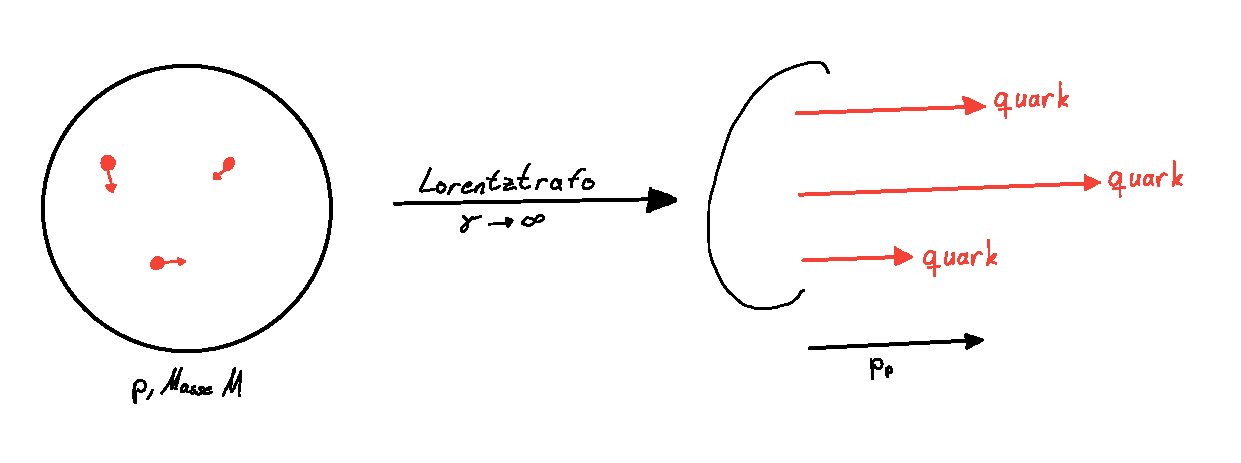
\includegraphics[width=.6\textwidth]{imgs/ep5-fig-6-7.pdf}
\caption{Strukturskizze eines Protons\label{fig:6.7}}
\end{figure}

\ni Aus \autoref{fig:6.7}: alle Massen und Transversalimpulse sind vernachlässigbar\\
Quark-Impuls:
\begin{align}
p_i = \xi_i p_p= \xi_i \lb \gamma M , \gamma M, 0, 0\rb 
\end{align}

\item[$\lt$] ep-Streuung $\hat{=}$ elastische eq-Streuung

\begin{figure}[!ht]
\centering
    \begin{tikzpicture}
        \begin{feynman}
            \vertex (a1);
            \vertex[right = 3cm of a1] (a2);
            \vertex[above right = 3cm of a2] (b1);
            \vertex[below right = 3cm of a2] (c1);
            
            \diagram*{
            (a1) -- [fermion, edge label = $q_i(p_i)$] (a2),
            (a2) -- [boson, edge label = $\gamma(q)$] (b1),
            (a2) -- [fermion, edge label = $q_f(p_f)$] (c1),
            };
        \end{feynman}
    \end{tikzpicture}
\caption{Feynmandiagramm zur Quarkstreeung\label{fig:6.8}}
\end{figure}

\begin{align}
p_f^2 = \lb  p_i + q\rb ^2 =p_i^2 - Q^2 + 2p_{i_\mu}q^\mu \nonumber \\
2p_{i,\mu} q^\mu = 2 \xi_i p_{p,\mu} q^\mu \overset{!}{=}Q^2 \nonumber\\
\boxed{ \xi_i = \frac{Q^2}{2 p_{i,\mu}q^\mu} = \frac{Q^2}{2 M \nu} = x }
\end{align}
\item[$\Ra$] $x=$ Anteil an p-Impuls, den das getroffene Quark trägt!
\end{itemize}
\item Beobachtung 3\\
$F_{1,2} \lb x, Q^2\rb  \approx F_{1,2}\lb x\rb $ ergeben \glqq Quark-Dynamik im Nukleon\grqq{}\\
Vereinfacht:
\begin{align}
\boxed{ \sigma \lb  e, p \rb   = \sum_{q \in p } \sigma \lb eq_i \rb   q_i\lb x\rb }
\end{align}
\begin{compactitem}
\item[mit] $q_i(x)$: \glqq Parton-Verteilungsfunktion\grqq{} (PDF)
\item[] $\sigma \lb ep\rb , \ \sigma\lb eq_i\rb $: eigentlicher differentieller WQ
\end{compactitem}
\tb{\glqq Parton\grqq}: Quark oder Gluon\\
für $q_i$ mit $x$ im Parton:
\begin{align}
\boxed{q_i\lb x\rb  = \dfrac{\lb WS\rb }{x}}
\end{align}
\end{itemize}

\vorlesung{12. Januar 2018}

\begin{figure}[!ht]
\centering
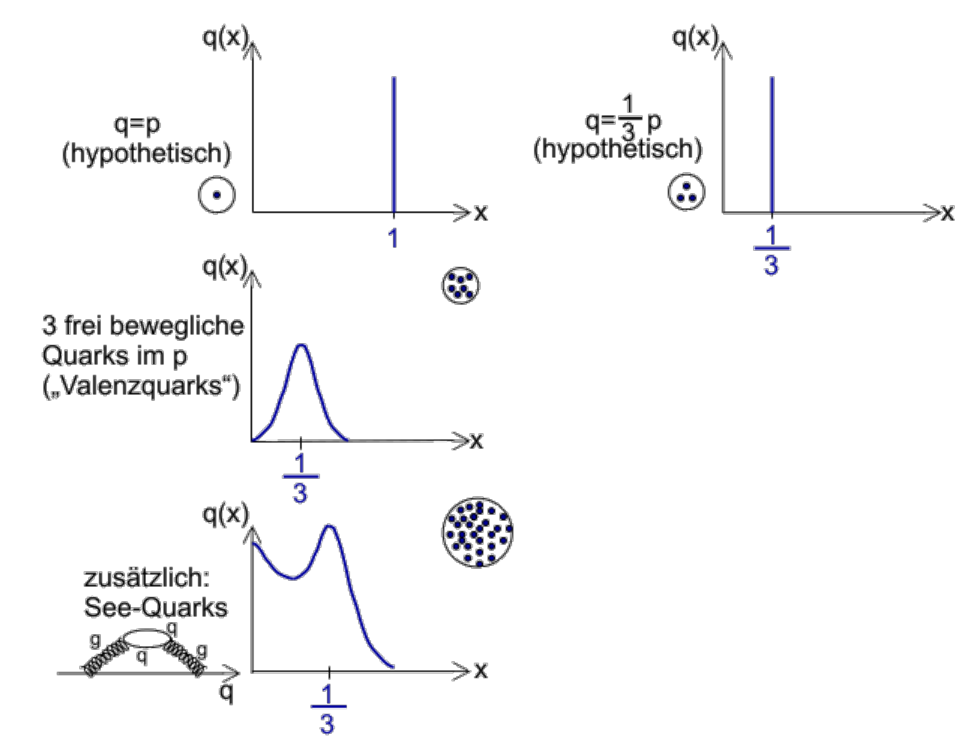
\includegraphics[width=.9\textwidth]{imgs/ep5-fig-6-9.pdf}
\caption{Erwartete Verteilungen für $q_i(x)$\label{fig:6.9}}
\end{figure}
\begin{itemize}
\newpage
\item \tb{Beobachtung 4}\\
$F_1$-Term im WQ kommt vom magnetischen Moment des Targets
\begin{itemize}
\item[$\Ra$] Erwartung:
\begin{align}
F_1\lb  x, Q^2\rb  = \begin{cases}0, \text{ wenn Spin}(q) = 0\\ 
\frac{F_2\lb x, Q^2\rb }{2x}, \text{ wenn Spin}(q) = \frac{1}{2} \end{cases}
\end{align}
\item[$\Ra$] Messung (Callen-Gross-Relation):
\begin{align}
\boxed{ 2xF_1\lb x, Q^2\rb  = F_2 \lb  x, Q^2\rb  }
\end{align}
$\ra$ Quarks sind Fermionen
\end{itemize}
\item \tb{Beobachtung 5}
\begin{align}
\int_0^1 \sum_{q\text{ in } p} x q_i(x) \Pa x \approx 0.5 \neq 1
\end{align}
1 erwartet, wenn nur Quarks q im Proton p wären.\\
$\Ra$ weitere Partonen = Gluonen in p
\newpage

\item \tb{Beobachtung 6}\\
Skaleninvarianz ist verletzt $\Ra$ Effekt der starken WW

\begin{figure}[!ht]
\centering
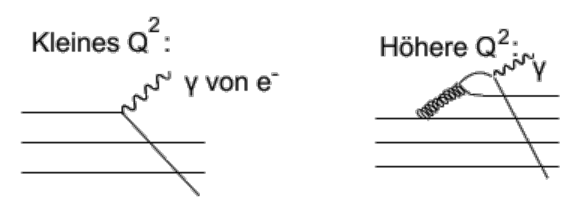
\includegraphics[width=.6\textwidth]{imgs/ep5-fig-6-10.pdf}
\caption{Verschiebung der Partonen-Verteilung mit zunehmenden $Q^2$ zu kleinen $x$\label{fig:6.10}}
\end{figure}
\end{itemize}

\chapter{Die starke Wechselwirkung}
\begin{itemize}
\item[$\ra$]  bindet Nukleonen im Atomkern
\item[$\ra$] bindet Quarks in Hadronen
$\Ra$ Starke WW ist auf Quark/Gluon-Niveau theoretisch exakt beschreibbar
\end{itemize}
\section{Grundlegende Struktur}
Theorie der starken WW: Quantenchromodynamik\\
\glqq chromo\grqq{} wegen der Farbe (von Farbladungen)
\begin{figure}[!ht]
\centering
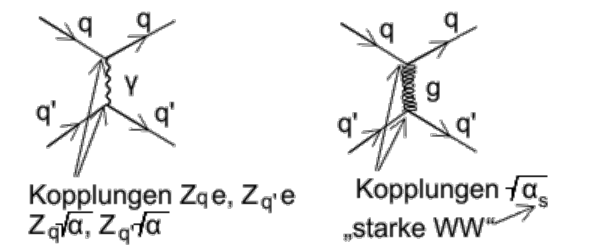
\includegraphics[width=.6\textwidth]{imgs/ep5-fig-7-1.pdf}
\caption{Feynmandiagramme zum Vergleich der starken und elm. WW \label{fig:7.1}}
\end{figure}
\begin{itemize}
\item[$\lt$] Gluonen sind masselos und koppeln an Farbladungen
\item[$\lt$] Es gibt 3 Farbladungen: r = rot, g = grün und b= blau
\item Theoretischer Hintergrund: Lokale Eichinvarianz\\
$\Ra$ fordere Invarianz unter:
\begin{align}
\text{elm. } & \Psi \ra \underbrace{e^{i\Phi\lb x_\mu\rb  } \Psi}_{\in Li(1)} & \Ra \ 1 \text{ \glqq Eichfeld\grqq{} = Photon}\\
\text{stark } & \Psi \begin{pmatrix}
r\\g\\b\end{pmatrix} \ra \underbrace{C\lb x_\mu\rb }_{\in SU(3)} \Psi \begin{pmatrix}r\\g\\b\end{pmatrix} & \Ra \ 8 \text{ Eichfelder = Gluonen, farbgeladen}
\end{align}
\item \tb{Farbladungen}
\begin{itemize}
\item[$\lt$] alle Leptonen, $\gamma$, $Z$, $W^{\pm}$ = 0
\item[$\lt$] alle Quarks: r,g,b
\item[$\lt$] alle Antiquarks: $\mr{\bar{r}, \bar{g}, \bar{b}}$
\item[$\lt$] alle Gluonen: $\mr{r\bar{g}, b \bar{r}, \dots}$
\newpage
\begin{figure}[!ht]
\centering
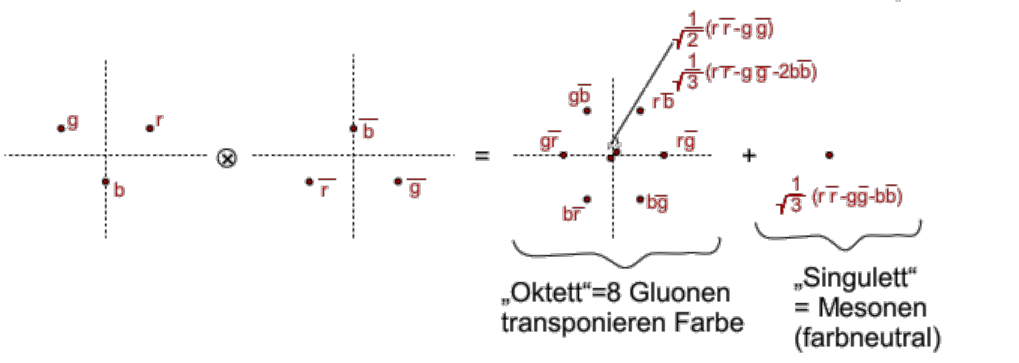
\includegraphics[width=.75\textwidth]{imgs/ep5-fig-7-2.pdf}
\caption{Kombination von Farbe und Antifarbe\label{fig:7.2}}
\end{figure}

\end{itemize}
\item Hadronen sind farbneutrale gebundene Systeme
\begin{itemize}
\item[$\lt$] Mesonen $\ket{q\bar{q}}$
\item[$\lt$] Baryonen $\ket{qqq}$
\item[$\lt$] \glqq Pentaquarks\grqq{} $\ket{qqqq\bar{q}}$
\item[$\lt$] \glqq Glueballs\grqq{} $\ket{gg}, \ \ket{ggg}$
\item Achtung Pentaquarks und Glueballs konnten noch nicht nachgewiesen werden!
\begin{figure}[!ht]
\centering
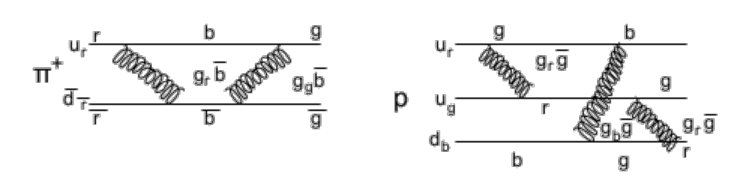
\includegraphics[width=.75\textwidth]{imgs/ep5-fig-7-3.pdf}
\caption{Skizze zur Farbladungserhaltung an jedem Vertex\label{fig:7.3}}
\end{figure}
\end{itemize}
\item Gluonen tragen Farbe

\begin{figure}[!ht]
\centering
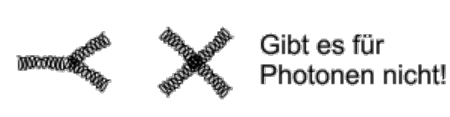
\includegraphics[width=.4\textwidth]{imgs/ep5-fig-7-4Gluonen.pdf}
\caption{Selbstwechselwirkung von Gluonen\label{fig:7.glue}}
\end{figure}

\item Farbgeladenen frei Teilchen (Quarks, Gluonen, Diquarks, \dots ) gibt es nicht\\
$\lt$ Confinement (\glqq Eingeschlossenheit\grqq)
\end{itemize}
\newpage
\section{Evidenzen für Gluonen und Farbe}
\begin{itemize}
\item \tb{Gluonen}
\begin{enumerate}
\item \tb{Tiefinelastische eN-Streuung}
\begin{align}
\int_0^1 \sum{q \text{ in } p } x q_i (x) \Pa x \approx 0.5
\end{align}
\begin{itemize}
\item[$\Ra$] Weitere \glqq Teilchensorte\grqq{} im Nukleon, mit der $e^-$ nicht wechselwirkt
\item[$\Ra$] elektrisch neutral
\end{itemize}
\item \tb{Jets}\\
\glqq Teilchenbündel\grqq\ in Richtung von Quarks oder Gluonen im Endzustand

\begin{minipage}[c]{.39\textwidth}
\captionsetup{type=figure}
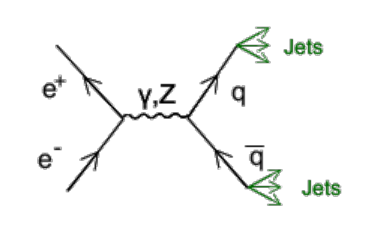
\includegraphics[width=\textwidth]{imgs/ep5-fig-7-4.pdf}
\captionof{figure}{Bsp.1: Feynmandiagramm für $e^+e^- \rightarrow q\bar{q}$ \label{fig:7.4}}
\end{minipage}
\begin{minipage}[c]{.39\textwidth}
\captionsetup{type=figure}
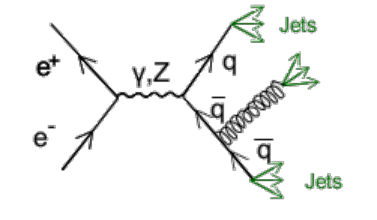
\includegraphics[width=\textwidth]{imgs/ep5-fig-7-5.pdf}
\captionof{figure}{Bsp.2: Feynmandiagramm für $e^+e^- \rightarrow q\bar{q}g$ \label{fig:7.5}}
\end{minipage}

\begin{itemize}
\item[$\rightarrow$] Entstehung von Jets oder auch von Baryonen
\item[$\rightarrow$] nur möglich, wenn einer der Jets von einem Gluon stammt
\item[$\rightarrow$] entdeckt 1979 am DESY
\end{itemize}

\begin{minipage}[c]{.39\textwidth}
\captionsetup{type=figure}
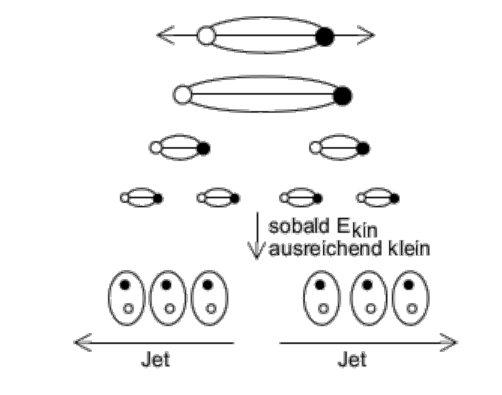
\includegraphics[width=\textwidth]{imgs/ep5-fig-7-6.pdf}
\captionof{figure}{Jet-Entstehung: für $e^+e^-$ entstehen 3 Jets \label{fig:7.6}}
\end{minipage}
\begin{minipage}[c]{.39\textwidth}
\captionsetup{type=figure}
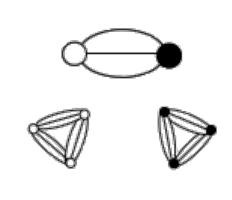
\includegraphics[width=\textwidth]{imgs/ep5-fig-7-7.pdf}
\captionof{figure}{Baryonenenstehung\\ aus Gluon-Jet \label{fig:7.7}}
\end{minipage}

\end{enumerate}
\end{itemize}
\newpage
\begin{itemize}
\item \tb{Farbe}
\begin{itemize}
\item[1.] \tb{Das $\Delta^{++}$-Baryon ($\Delta^{++}(1232))$}\\
Produktion z.B. $\nu_\mu p\rightarrow\mu^-\Delta^{++}$
\begin{align}
\ket{\Delta^{++}}=\ket{u\uparrow u\uparrow u\uparrow};\ J^p=(\frac{3}{2})^+
\end{align}
$\rightarrow$ Bahndrehimpuls $L=0$ (leichterer Q=2e-Baryon)\\
$\rightarrow$ Symmetrische Wellenfunktion (Flavour, Spin, Ort)
$\rightarrow$ symm. unter Tausch von 2 identischen Fermionen $\thor$ Pauli-Prinzip\\
$\rightarrow$ Lösung: $\ket{u_r\uparrow u_b\uparrow u_s\uparrow}$ mit antisymmetrischen Farb-Wellenfkt. %bin nicht sicher ob u_r stimmt konnte es nicht genau lesen!
\item[2.] \tb{WQ für $e^+ e^- \rightarrow q\bar{q} \rightarrow$ Hadronen} (z.B.: Abb.\ref{fig:7.8})
\begin{figure}[!ht]
\centering
\includegraphics[width=.45\textwidth]{imgs/ep5-fig-7-8.pdf}
\caption{Feynmandiagramm zu $e^+e^-\rightarrow f\bar{f}$ \label{fig:7.8}}
\end{figure}

Diese Reaktion $e^+e^-\rightarrow \underbrace{f\bar{f}}_{\text{Fermion/Antifermion-Paar}}$ ist möglich wenn
\begin{align*}
s=(E_{cms})^2 > (2m_f)^2
\end{align*}
$Z^0$-Austausch dominant bei $\sqrt{s}=M_z$, aber klein bei $\sqrt{s}\approx \mathcal{O}(10\,keV)$\\
Wirkungsquerschnitt:
\begin{align}
\frac{\Pa \sigma}{\Pa \Omega}\sim \frac{Z^2_f\alpha^2}{s} (1+cos^2\theta)
\end{align}
Betrachte
\begin{align}
\Pa\frac{\sigma^{Had}}{\Pa\omega}=\sum_{\sqrt{s}>2m_{a_i}\footnotemark}\frac{\Pa \sigma^{a_i}}{\Pa \Omega}
\end{align}
Summenindex hat Schwelle bei $\sim$ 1\,GeV für strange-, $\sim$ 3\,GeV für charme-, $\sim$ 10\,GeV für bottom- und $\sim$ 350\,GeV für top-Quarks.\\
Verwende $e^+e^-\rightarrow\mu^+\mu^-$ als \grqq Eichreaktion\grqq:
\begin{align}
R_\mu=\frac{\nicefrac{d\sigma^{Had}}{d\Omega}}{\nicefrac{d\sigma^\mu}{d\Omega}}=\sum_{\sqrt{s}>2M_{a_i}}Z^2_{a_i}
\end{align}
Summieren über alle Farbzustände (r,g,b)$\rightarrow$ Faktor 3\\
Erhalten also:
\begin{align}\label{eq:7.8}
R_\mu = 3 \bigg[\underbrace{\underbrace{\underbrace{\underbrace{\stackrel{u}{\left(\frac{2}{3}\right)^2}+\stackrel{d}{\left(\frac{1}{3}\right)^2}}_{\sqrt{s}\geq 150\,MeV}+\stackrel{s}{\left(\frac{1}{3}\right)^2}}_{\sqrt{s}\geq 1\,GeV}+\stackrel{c}{\left(\frac{2}{3}\right)^2}}_{\sqrt{s}\geq 3\,GeV}+\stackrel{b}{\left(\frac{1}{3}\right)^2}}_{\sqrt{s}\geq 10\,GeV}+\stackrel{t}{\left(\frac{2}{3}\right)^2}\bigg]
\end{align}
\begin{figure}[!ht]
\centering
\includegraphics[width=.5\textwidth]{imgs/ep5-fig-7-9.pdf}
\caption{Graphische Veranschaulichung der Geichung \ref{eq:7.8} \label{fig:7.9}}
\end{figure}
\begin{itemize}
\item[$\rightarrow$] Faktor 3 durch Messung bestätigt
\item[$\rightarrow$] Es gibt Farbladungen und davor genannt
\end{itemize}
\end{itemize}
\end{itemize}
\section{Die starke Kopplung: Confinement und Asymptotic-Freedom}
Die Kopplungsstärke von Wechselwirkungen hängt von $Q^2$ ab. Grund sind höhere Ordnungen der Störungsreihe
\begin{itemize}
\item Für elektromagnetische WW (QED):
\begin{figure}[!ht]
\centering
\includegraphics[width=.65\textwidth]{imgs/ep5-fig-7-10.pdf}
\caption{Höhere Ordnungen elektromagnetischer Wechselwirkung \label{fig:7.10}}
\end{figure}

$\Rightarrow$ Abschirmung:

\begin{figure}[!ht]
\centering
\includegraphics[width=.5\textwidth]{imgs/ep5-fig-7-11.pdf}
\caption{Dipolwolke um das rechte Elektron schirmt das linke, einfliegende Elektron ab \label{fig:7.11}}
\end{figure}

$\rightarrow$ Ladung umso größer, je \grqq näher man kommt \grqq\, d.h. desto größer $Q^2$
\begin{align}
\Rightarrow\alpha=\alpha(Q^2)=
\begin{cases}
\nicefrac{1}{137} & (Q^2=0)\\
\nicefrac{1}{128} & (Q^2=M^2_z)
\end{cases}
\end{align}

\item Für starke WW (QCD):

\begin{figure}[!ht]
\centering
\includegraphics[width=.5\textwidth]{imgs/ep5-fig-7-12.pdf}
\caption{Höhere Ordnungen der starken Wechselwirkung \label{fig:7.12}}
\end{figure}
\begin{itemize}
\item[$\rightarrow$] dominant!
\item[$\Rightarrow$] $\alpha_s(Q^2)$ wird mit $Q^2$ kleiner!
\begin{align}
\Rightarrow \text{\fbox{$\alpha_s(Q^2)=\frac{12\pi}{(33-2N_f\footnotemark)ln\frac{Q^2}{\Lambda^2\footnotemark}}+h.O.$}} 
\end{align}
\begin{compactitem}
\item[mit] $N_f$: Zahl der Quarkflavours
\item[] $\Lambda$: in QED-Skala $\sim$ 250\,MeV
\end{compactitem}
\begin{align}
\alpha_s(Q^2)=
\begin{cases}
0,1185 & (Q^2=M^2_z)\\
0,3 & (Q^2=m^2_\tau)\\
>1 & (Q^2\leq 0,1\, GeV^2)
\end{cases}
\end{align}
\item[$\Rightarrow$] \textbf{Grenzfläche:}
\begin{itemize}
\item $Q^2\rightarrow 0:\ \alpha_s\rightarrow\infty$
\begin{itemize}
\item[$\rightarrow$] keine Störungsrechnung
\item[$\rightarrow$] keine freien Farbladungen
\item[$\rightarrow$] \grqq Confinement \grqq\
\end{itemize}
\item $Q^2\rightarrow \infty:\ \alpha_s \rightarrow 0$
\begin{itemize}
\item[$\rightarrow$] Störungsrechnung (QCD)
\item[$\rightarrow$] \grqq quasi-freie\grqq{} Quarks in tiefinelastischer Streuung
\item[$\rightarrow$] \grqq Asymptotic-Freedom\grqq\
\end{itemize}
\end{itemize}
\end{itemize}
\end{itemize}

\vorlesung{19. Januar 2018}

\section{Aufbau der Hadronen}
Quark-Gluon-Kopplung unabhängig von Quark-Flavour (u,d,s,c,t,b)
\begin{itemize}
\item[$\ra$] Hadron-Zustände nur von Bindungszustand ($L,J,n$) abhängig?
\item[$\ra$] Nein:            Effekt
\item[$\ra$] Quark-Massen     groß
\item[$\ra$] Quark-Ladungen   klein
\item \tb{Isospin-Symmetrie}\\
u- und d-Quarks haben etwa gleiche Massen (einige MeV)
\begin{itemize}
\item[$\Ra$]u$\leftrightarrow$d lässt die Hadronzustände \textbf{näherungsweise} invariant
\item[$\Ra$] Formel: starke WW \textbf{näherungsweise} invariant unter:
\begin{align*}
\left(\begin{array}{c}u\\d\end{array}\right)\rightarrow SU(2)\left(\begin{array}{c}u\\d\end{array}\right)\\
\Rightarrow \text{\grqq Isospin\grqq}\\
\ket{u}=I, I=\frac{1}{2}, \ket{_3=\frac{1}{2}}\\
\ket{d}=I, I=\frac{1}{2}, \ket{_3=-\frac{1}{2}}
\end{align*}
\item[$\Rightarrow$] Es gibt \grqq Sätze\grqq\ von Hadronen die aus $\stackrel{\leftrightarrow}{u},\stackrel{\leftrightarrow}{d}$ bestehen und mit $SU(2)$-Isospin in  sich selbst übergehen $\rightarrow$ \grqq Isospin-Multipletts\grqq
\begin{itemize}
\item gleiches $I$
\item $\sim$ gleiche Massen
\item Ladung = $f(I_3)$
\end{itemize}
\end{itemize}
$\Rightarrow$ Beispiel: Mesonen

\begin{figure}[!ht]
\centering
\includegraphics[width=.75\textwidth]{imgs/ep5-fig-7-13.pdf}
\caption{Isospinzusammensetzung bei Mesonen \label{fig:7.13}}
\end{figure}

Entstehendes Meson aus
\begin{align*}
L=0;\ S=0\rightarrow J^{PC}=0^{-+}:\ \pi^+,\pi^-,\pi^0\\
L=0;\ S=1\rightarrow J^{PC}=1^{--}:\ \rho^+,\rho^-,\rho^0\\
(M_\rho\approx 770\,MeV)
\end{align*}
\item \tb{Erweiterung auf 3 Quark-Flavours:}\\
$(u,d,s)$, $SU(2)\rightarrow SU(3),d.h.:$
\begin{figure}[!ht]
\centering
\includegraphics[width=.75\textwidth]{imgs/ep5-fig-7-14.pdf}
\caption{Erweiterung der Isopspinsymmetrie um den dritten Quarkflavour s \label{fig:7.14}}
\end{figure}
\begin{align}\begin{split}
A&=\frac{1}{\sqrt{2}}(u\bar{u}-d\bar{d})=\ket{\pi^0}\\
B&=\frac{1}{\sqrt{6}}(u\bar{u}+d\bar{d}-2s\bar{s})\approx\ket{\eta}\\
C&=\frac{1}{\sqrt{3}}(u\bar{u}+d\bar{d}+s\bar{s})\approx\ket{\eta^\prime}
\end{split}\end{align}
Wobei $B$ und $C$ mischen!

Wegen $m_s\gg m_{u,d}$: Massen \textbf{nicht} ähnlich $(M_\pi=139\,\mr{MeV},\ M_K=485\,\mr{MeV})$
\begin{itemize}
\item[$\Rightarrow$] SU(3) keine \grqq gute\grqq Symmetrie, aber bietet gute Ordnungsschema, auch für Baryonen
\end{itemize}
\item \tb{Erweiterung auf c-Quarks}
\begin{itemize}
\item[$\rightarrow$]$SU(3)\rightarrow SU(4)$
\item[$\rightarrow$] 3D-Multipletts
\item[$\rightarrow$] wichtig als Ordnungsschema
\end{itemize}
\end{itemize}

\section{Erzeugung und Zerfall von Hadronen}
\begin{itemize}
\item \tb{Erzeugung}\\
In hadronischen Reaktionen
\begin{itemize}
\item[$\ra$] \grqq Umwandlung von Quark-Linien\grqq\, z.B. $\pi^- p\rightarrow\pi^0 n$

\begin{figure}[!ht]
\centering
\includegraphics[width=.5\textwidth]{imgs/ep5-fig-7-15.pdf}
\caption{Feynmandiagramm zur Umwnadlungsreaktion \label{fig:7.15}}
\end{figure}

\item[$\ra$] Erzeugung/Vernichtung von Quark-Antiquark-Teilchen\\
z.B. $\pi^- p \rightarrow \Delta^0(1232)\rightarrow\pi^0 n$

\begin{figure}[!ht]
\centering
\includegraphics[width=.5\textwidth]{imgs/ep5-fig-7-16.pdf}
\caption{Feynmandiagramm zur $\pi^0n$ Erzeugung\label{fig:7.16}}
\end{figure}

z.B. $\pi^- p \rightarrow \Lambda k^0$
\begin{figure}[!ht]
\centering
\includegraphics[width=.5\textwidth]{imgs/ep5-fig-7-17.pdf}
\caption{Assoziierte Produktion \label{fig:7.17}}
\end{figure}

\item[$\ra$] Inelastisch, z.B. in Jet-Bildung (\grqq Fragmentation\grqq, \grqq Hadronisation\grqq)
\end{itemize}
In $e^+ e^-$-Streuung:
\begin{itemize}
\item[$\ra$] Hadronische $q\bar{q}$-Resonanzen, z.B. $e^+ e^- \rightarrow \nicefrac{J}{\Psi}$

\begin{figure}[!ht]
\centering
\includegraphics[width=.5\textwidth]{imgs/ep5-fig-7-18.pdf}
\caption{Inelastische Erzeugung von $\nicefrac J\Psi$ \label{fig:7.18}}
\end{figure}

Auch für
\begin{align*}
u\bar{u},d\bar{d}: \rho^0\\
s\bar{s}: \phi\\
b\bar{b}: \gamma 
\end{align*}
\item[$\ra$] $e^+ e^- \rightarrow qq(g)$, Jet-Bildung
\end{itemize}
%hier ist iwas zerschossenes es sieht auf jeden fall kackeeee aus
\item \tb{Zerfälle}\\
Alle 3 WW kommen vor
\begin{itemize}
\item[1.] starke WW, z.B. $\rho^0\rightarrow\pi^+\pi^-$
\begin{figure}[!ht]
\centering
\includegraphics[width=.5\textwidth]{imgs/ep5-fig-7-19.pdf}
\caption{Zerfall von $\rho$ durch die starke WW \label{fig:7.19}}
\end{figure}

wenn erlaubt: dominant\\
Typisch : $\Gamma\approx 100...150\,\mr{MeV}$, $\tau\approx 10^{-23}\,\mr{s}$
\item[2.] Elektromagnetische WW (wenn Zerfall über starke WW nicht möglich ist)\\
z.B. $\pi^0\rightarrow\gamma\gamma$ (vgl. Abb. \ref{fig:7.20})

\begin{figure}[!ht]
\centering
\includegraphics[width=.5\textwidth]{imgs/ep5-fig-7-20.pdf}
\caption{Zerfall von $\pi^0$ durch elektromagnetische WW \label{fig:7.20}}
\end{figure}

$\pi^0$ leichteres Hadron, starker Zerfall nicht möglich
$\tau\approx 10^{-16}\,\mr{s}$\\
auch: $\sum^0\rightarrow \Lambda\gamma$
\item[3.] schwache WW (wenn starke und elm. verboten sind)\\
Insbesondere für leichte/leichteste Hadronen mit $S\neq 0,C\neq 0, B\neq 0$\\
z.B. $K^+\rightarrow \mu^+\nu_\mu$ (vgl. Abb.\ref{fig:7.21})

\begin{figure}[!ht]
\centering
\includegraphics[width=.5\textwidth]{imgs/ep5-fig-7-21.pdf}
\caption{Zerfall von $K^+$ durch Austausch eines $W^+$-Bosons \label{fig:7.21}}
\end{figure}

genauso: $\Pi^+(s\leftrightarrow d)$
\item[$\rightarrow$] Spezieller Fall: Quarkonium\\
Zustände aus einem Quark und seinem Antiquark, Mesonen ohne elektrische Ladung oder Flavour.

Für die Lebensdauer gilt: $\tau \sim 0.7\cdot 10^{-20}\,s$ 

\begin{figure}[!ht]
\centering
\includegraphics[width=.5\textwidth]{imgs/ep5-fig-7-22.pdf}
\caption{Feynmandiagramm zum Quarkonium \label{fig:7.22}}
\end{figure}
\end{itemize}
\end{itemize}

\vorlesung{25. Januar 2018}

\chapter{Die Schwache Wechselwirkung}
Bisher haben wir gesehen:
\begin{itemize}
\item $\beta$-Zerfälle von Kernen
\item Hadron-Zerfälle
\item Neutrinos
\end{itemize}
\tb{Jetzt: }Systematisch
\section{Grundlegende Struktur}
\begin{itemize}
\item WW durch Austausch von Bosonen (wie QED, QCD)
\item Austauschteilchen sind massiv und geladen:\\
$W^\pm$, $M_W = 80.4\,$GeV\\
$Z^0$, $M_Z = 91.2$\,GeV
\item koppelt an \tb{alle} Fermionen (einzige WW von Neutrinos)
\item Immer: $W$- oder $Z$-Propagator
\begin{align}
\boxed{\mc{M} \sim \frac{1}{Q^2 + M_{W,Z}^2} \, \Ra \, \sigma,\ \Gamma \overset{Q^2 \ll M_{W,Z}^2}{\sim} \frac{1}{M_{W,Z}^4}}
\end{align}
Nenner $M_{W,Z}^4$ ist der Grund dafür, warum die schwache WW schwach ist.
\item Eichstruktur (angedeutet)
\begin{align}
\underbrace{SU(2)\begin{pmatrix}\cdot\\ \cdot\end{pmatrix}_L}_{\substack{\text{Eichbosonen:}\\W^-, W^0, W^+}} \hspace*{1cm} \underbrace{U(1) (\cdot)_R}_{\substack{\text{Eichboson:}\\B}}
\end{align}
$SU(2)$ ist linkshändig, $U(1)$ dagegen rechtshändig.\\
Die Eichbosonen $W^0$ und $B$ können mischen. Es gilt dafür:
\begin{align}
\begin{pmatrix}
Z^0 \\ \gamma
\end{pmatrix} = \begin{pmatrix}
\cos \theta_W & - \sin \theta_W\\  \sin \theta_W & \cos \theta_W
\end{pmatrix} \begin{pmatrix}
W^0 \\ B
\end{pmatrix}
\end{align}
(\glqq elektroschwache Vereinigung\grqq{})
\begin{compactitem}
\item[mit] $\theta_W$: Weinberg-Winkel
\item[] $\sin^2 \theta_W \approx 0.222$
\item[] $\Ra$ $Z^0$ hat \glqq elektromagnetischen Anteil\grqq{}
\end{compactitem}
\item Higgs-Boson:\\
Notwendig, um massive Eichbosonen zu erklären, ohne Eichsymmetrie zu verletzen
\end{itemize}

\section{Der geladene Strom}

$W^\pm$-Austausch, koppelt an alle Fermionen:

\begin{figure}[!ht]
\centering
\includegraphics[width=.5\textwidth]{imgs/ep5-fig-8-1.pdf}
\caption{$W$-Kopplung an ein Lepton und das zugehörige Neutrino bzw. an ein Quark \label{fig:8.1}}
\end{figure}

\begin{itemize}
\item Kopplungsstärke
\begin{align}
g_W = \frac{e}{\sin \theta_W}
\end{align}
$\Ra$ \tb{stärker} als bei elm. WW!
\item \tb{Quark-Mischung}\\
Beobachtet z.B. bei Zerfall der leichtesten Mesonen/Baryonen mit $S\neq 0$

\begin{figure}[!ht]
\centering
\includegraphics[width=.5\textwidth]{imgs/ep5-fig-8-2.pdf}
\caption{Quark-Mischung am Beispiel $\Lambda^0 \ra n \pi^0$\label{fig:8.2}}
\end{figure}
\newpage
Erklärung:
\begin{framed}
\begin{center}
Quark-EZ der schwachen WW $\neq$ Quark-EZ der starken WW
\end{center}
\end{framed}
QM: Beide EZ-Vektoren durch unitäre Transformation verknüpft. Für d,s ergibt sich:
\begin{align}
\boxed{ \underbrace{\begin{pmatrix}
d^\prime \\ s^\prime 
\end{pmatrix}}_\text{schwach} = \underbrace{\begin{pmatrix}
\cos \theta_C & \sin \theta_C\\ -\sin\theta_C & \cos \theta_C \end{pmatrix}}_\text{Cabibbo-Matrix} \underbrace{\begin{pmatrix}
d \\ s
\end{pmatrix}}_\text{stark}
 }
\end{align}
Hierbei ist $\theta_C$ der sogenannte Cabibbo-Winkel.
\begin{align*}
\sin \theta_C \approx 0.22, \sin^2 \theta_C \approx 0.05
\end{align*}
\begin{itemize}
\item[$\Ra$] Geladener Strom hat Terme:
\begin{align}
\begin{pmatrix}
u \\ c
\end{pmatrix}^\top U_\mr{Cab} \begin{pmatrix}
d \\ s
\end{pmatrix}=\quad \begin{cases}\quad 
\lno \begin{matrix}
ud \cdot \cos \theta_C & +\\ cs \cdot \cos\theta_C & +
\end{matrix} \rrb \labs \mc{M}\rabs^2 \sim \cos^2 \theta_C \approx 0.95\\ \ \\
\quad \lno \begin{matrix}
us \cdot \sin \theta_C & -\\ cd \cdot \sin\theta_C & -
\end{matrix} \rrb \labs \mc{M}\rabs^2 \sim \sin^2 \theta_C \approx 0.05 \end{cases}
\end{align}
\item[$\lt$] $U_\mr{Cab}$ kann auch als Mischung von $(u,c)$ interpretiert werden
\item[$\Ra$] \glqq Nicht diagonale\grqq{} Terme sind mit Faktor 20 unterdrückt.
\begin{figure}[!ht]
\centering
\includegraphics[width=.5\textwidth]{imgs/ep5-fig-8-3.pdf}
\caption{Offidiagonale ($\sin \theta_C$ Zerfälle unterdrückt \label{fig:8.3}}
\end{figure}

$\Ra$ Verallgemeinerung auf 3 Quark-Familien
\begin{align}
\boxed{ \begin{pmatrix}
d^\prime \\ s^\prime \\ b^\prime 
\end{pmatrix} = U(3) \cdot \begin{pmatrix}
d \\ s\\ b
\end{pmatrix} }
\end{align}
$U(3)$ = unitäre Matrix, genannt Cabibbo-Kobayashi-Maskawa-Matrix (CKMM)
\begin{itemize}
\item[$\lt$] 3 reelle Parameter (\glqq Drehwinkel\grqq{})
\item[$\lt$] komplexe Phase
\item[$\lt$] Beträge der Matrixelemente
\begin{align}
\begin{pmatrix}
0.974 & 0.225 & 0.004 \\
0.225 & 0.973 & 0.041\\
0.009 & 0.040 & 0.999
\end{pmatrix} \approx \begin{pmatrix}
U_\mr{Cab} & \begin{matrix}
0.004 \\ 0.041
\end{matrix} \\
\begin{matrix}
0.009 & 0.040
\end{matrix} & 0.999
\end{pmatrix}
\end{align}
sehr stark diagonaldominant
\item[$\ra$]  Aus unterer Zeile
\begin{align*}
\Gamma \lb  t \ra d\rb : \Gamma \lb t \ra s\rb  : \Gamma\lb t \ra b\rb  = (0.009)^2 : (0.040)^2 : (0.999)^2
\end{align*}

\begin{figure}[!ht]
\centering
\includegraphics[width=.5\textwidth]{imgs/ep5-fig-8-4.pdf}
\caption{Feynmandiagramme zu WW bezüglich der unteren Zeile der CKMM \label{fig:8.4}}
\end{figure}
\end{itemize}
\end{itemize}
\end{itemize}
\section{Paritätsverletzung in der schwachen WW}
Erinnerung: Parität ist verletzt, wenn
\begin{align}\begin{split}
&\hat{P}^\dagger \Ham_{WW} \hat{P} \neq \Ham_{WW}\\
\Ra \mc{M}_P &= \braket{\Psi_f | \hat{P}^\dagger \Ham_{WW} \hat{P} | \Psi_i}\\
& = \braket{\hat{P}\Psi_f | \Ham_{WW} | \hat{P} \Psi_i}\\
& \neq \braket{\Psi_f | \Ham_{WW} | \Psi_i}
\end{split}\end{align}
raumgespiegelten Prozess $\neq$ Wahrscheinlichkeit für ungespiegelten Prozess.

Bis $\sim$1955: Fester \glqq Glaube\grqq{} an Paritätserhaltung.\\Dann: Experiment von C.S. Wu (1956)
\begin{align*}
\underset{\text{Spin 5}}{^{60}_{27} Co} \ra \underset{\text{Spin 4}}{^{60}_{28} Ni^\star} + e^- + \bar{\nu}_e
\end{align*}

\begin{figure}[!ht]
\centering
\includegraphics[width=.5\textwidth]{imgs/ep5-fig-8-5.pdf}
\caption{Experiment zur Paritätsverletzung bei schwacher WW\label{fig:8.5}}
\end{figure}
\newpage
Achtung: $\hat{P} \vec{B} = \vec{B}$, $\hat{P} \vec{J} = \vec{J}$, $\hat{P}\vec{p} = - \vec{p}$
\begin{itemize}
\item[$\Ra$] Paritätsverletzung!
\item[$\Ra$] Interpretation $\bar{\nu}$ ist rechtshändig, denn:

\begin{figure}[!ht]
\centering
\includegraphics[width=.5\textwidth]{imgs/ep5-fig-8-6.pdf}
\caption{$\bar{\nu}$ ist rechtshändig, da die rechten Prozess unterdrückt ist \label{fig:8.6}}
\end{figure}
\item[$\Ra$] Schwache WW koppelt an linkshändige $\nu$'s und an rechtshändige $\bar{\nu}$'s\\
(1957 bestätigt in Goldhader-Experiment)

\begin{figure}[!ht]
\centering
\includegraphics[width=.65\textwidth]{imgs/ep5-fig-8-7.pdf}
\caption{Skizze zum Goldhader-Experiment \label{fig:8.7}}
\end{figure}

\item[$\lt$] $\underbrace{\text{maximale}}_{\begin{pmatrix}
\nu_l\\l\end{pmatrix}_L, \ \begin{pmatrix}
q^\prime \\ q \end{pmatrix}_L}$ $\underbrace{\text{Paritätsverletzung!}}_{\substack{(l)_R, \ (q)_R\\\text{Koppeln nicht an $W$}}}$
\item[$\Ra$] Bisher: Helizität $h$
\begin{align}
h = \frac{\vec{\sigma}\vec{p}}{\labs \vec{\sigma}\rabs \labs \vec{p} \rabs}
\end{align}
In der Theorie der schwachen WW entscheiden \glqq Chiralität\grqq{} $\hat{C}_{L,R}$
\begin{align*}
\ket{\Psi} = \ket{\Psi_L} + \ket{\Psi_R} = \hat{C}_L \ket{\Psi} + \underbrace{\hat{C}_R}_{= (1-\hat{C}_L)}\ket{\Psi}\\
\ket{\bar{\Psi}} = \ket{\bar{\Psi}_R} + \ket{\bar{\Psi}_L} = \hat{C}_L \ket{\bar{\Psi}} + \hat{C}_R\ket{\bar{\Psi}}
\end{align*}
Hierbei koppel $\ket{\Psi_L}$ und $\ket{\bar{\Psi}_R}$ an $W^\pm$\\
Helizität:
\begin{align*}
\ket{\Psi_L} = \sqrt{\frac{1+\beta}{2}} \ket{h=-1} + \sqrt{\frac{1-\beta}{2}} \ket{k=+1}\\
\ket{\Psi_R} = \sqrt{\frac{1+\beta}{2}} \ket{h=+1} + \underbrace{\sqrt{\frac{1-\beta}{2}} \ket{k=-1}}_{\substack{\text{\glqq falsche Helizität\grqq{}}\\\text{unterdrückt bei } \beta \ra 1\\\text{(insbesondere für $\nu$'s)}}}
\end{align*}
\item[$\Ra$] \tb{Beispiel: $\pi^+$-Zerfall}

\begin{figure}[!ht]
\centering
\includegraphics[width=.5\textwidth]{imgs/ep5-fig-8-8.pdf}
\caption{Helizitätsverletzung im $\pi^+$-Zerfall \label{fig:8.8}}
\end{figure}

\begin{align*}
\frac{\Gamma \lb  \pi^+ \ra e^+ \nu_e\rb }{\Gamma \lb  \pi^+ \ra \mu^+ \nu_\mu\rb  }= 1.2\cdot 10^{-4}
\end{align*}
Warum? Phasenraumfaktor ist viel größer für $\pi^+ \ra e^+ \nu_e$, weil $m_e\ll m_\mu$

\begin{figure}[!ht]
\centering
\includegraphics[width=.5\textwidth]{imgs/ep5-fig-8-9.pdf}
\caption{falsche Helizität für $e$, $\mu$ \label{fig:8.9}}
\end{figure}
\newpage

\begin{itemize}
\item[$\lt$] $\nu$ muss $h=-1$ haben
\item[$\lt$] $e$, $\mu$ muss $h=-1$ haben (Drehimpulserhaltung)
\begin{itemize}
\item[$\Ra$] $e$, $\mu$ hat \glqq falsche\grqq{} Helizität
\item[$\Ra$] unterdrückt mit $\frac{1 - \beta}{2}$\\
Faktor:
\begin{align}
\frac{m_e^2}{\lb M_\pi + m_e\rb ^2} \ll \frac{\mu_\mu^2}{\lb M_\pi + m_\mu \rb ^2}
\end{align}

\begin{align*}
\Gamma \lb  \pi^+ \ra e^+ \nu_e\rb  \ll \Gamma \lb  \pi^+ \ra \mu^+ \nu_\mu\rb 
\end{align*}
\end{itemize}
\end{itemize}
\end{itemize}

\section{CP-Symmetrie und CP-Verletzung}
\begin{itemize}
\item \tb{Erinnerung:}\\
$\hat{C}$ = Ladungskonjugation
\begin{align*}
\hat{C} \ket{\Psi} = \pm \ket{\bar{\Psi}}\\
\hat{C}\ket{\pi^0} = + \ket{\pi^0}\\
\hat{C}\ket{\pi^+ \pi^-} = \lb -1\rb ^2 \ket{\pi^+ \pi^-}
\end{align*}
\item \tb{CP-Transformation}
\begin{align}\begin{split}
\hat{C}\hat{P} \ket{\pi^0} = - \ket{\pi^0} \hspace*{1cm} (J^\mr{PC} = 0^{-+})\\
\hat{C}\hat{C} \ket{\gamma} \hspace*{1cm} (J^\mr{PC} = 0^{--})\\
\hat{C}\hat{P} \ket{\pi^+\pi^-} = (-1)^L \ket{\pi^+ \pi^-} \overset{\text{alle }L=0}{=} - \ket{\pi^+ \pi^-\pi^0}
\end{split}\end{align}
\newpage

\item \tb{$\hat{C}$- und $\hat{P}$-Transformatioen von Neutrinos}

\begin{figure}[!ht]
\centering
\includegraphics[width=.65\textwidth]{imgs/ep5-fig-8-10.pdf}
\caption{Skizze zur $C$- und $P$-Transformation \label{fig:8.10}}
\end{figure}

\begin{itemize}
\item[$\Ra$] $C$ ist maximal verletzt (wie $P$)
\item[$\Ra$] $CP$ könnte erhalten sein (fester \glqq Glaube\grqq{} bis 1964)
\end{itemize}
\item \tb{Entdeckung der $CP$-Verletzung} 1964 im $K^0$-System
\begin{align*}
\lno \begin{matrix}
\ket{K^0} = \ket{d\bar{s}}\\ \ket{K^0} = \ket{ s\bar{d}}
\end{matrix}\rrb\text{ können sich ineinander umwandeln}
\end{align*}

\begin{figure}[!ht]
\centering
\includegraphics[width=.5\textwidth]{imgs/ep5-fig-8-11.pdf}
\caption{Möglichkeiten zur $K^0$-Umwandlung \label{fig:8.11}}
\end{figure}

\begin{itemize}
\item[$\Ra$] Beobachtet werden $K^0$-$\bar{K}^0$-Mischungen
\item[$\Ra$] Konstruiere $CP$-Eigenzustände
\begin{align}
\lno \begin{matrix}
\hat{C} \ket{K^0} = \ket{\bar{K}^0}\\
\hat{P} \ket{K^0} = - \ket{K^0}
\end{matrix}\rrb \hat{C}\hat{P} \ket{K^0} = - \ket{\bar{K}^0}\nonumber \\
\lno \begin{matrix}
\hat{C} \ket{\bar{K}^0} = \ket{K^0}\\
\hat{P} \ket{\bar{K}^0} = - \ket{\bar{K}^0}
\end{matrix}\rrb \hat{C}\hat{P} \ket{\bar{K}^0} = - \ket{K^0}\nonumber \\
\boxed{\begin{matrix}
\ket{K_1} = \frac{1}{\sqrt{2}} \lb  \ket{K^0} - \ket{\bar{K}^0} \rb , & \hat{C}\hat{P} \ket{K_1} = \ket{K_1}\\
\ket{K_2} = \frac{1}{\sqrt{2}} \lb  \ket{K^0} + \ket{\bar{K}^0}\rb , & \hat{C}\hat{P}\ket{K_2} = - \ket{K_2}
\end{matrix}}
\end{align}
Wenn $CP$ erhalten.\\
$K_1$ zerfällt in $CP$-Eigenzustand mit $CP=+1$\\
$K_2$ zerfällt in $CP$-Eigenzustand mit $CP=-1$\\
Insbesondere:
\begin{align*}
K_1 \ra 2\pi \hspace*{1cm} &\lb \tau_1 = 0.9 \cdot 10^{-10}\,\mr{s}\rb \\
K_2 \ra 3 \pi \hspace*{1cm} &\underbrace{\lb  \tau_2 = 5.1\cdot 10^{-8}\mr{s}\rb }_{\substack{\text{Phasenraumeffekt}\\lb M_n - 2M_\pi \gg M_n - 3M_\pi)}}
\end{align*}
\tb{Experiment:}
\begin{figure}[!ht]
\centering
\includegraphics[width=.5\textwidth]{imgs/ep5-fig-8-12.pdf}
\caption{Skizze zum experimentellen Aufbau \label{fig:8.12}}
\end{figure}

Ergebnis:
\begin{align}
& \boxed{ K_2 \ra 2\pi \text{ mit } 0.23\,\% \text{ WS}}\\
& \Ra \ CP\text{-Verletzung}\nonumber
\end{align}
\item[$\lt$] $CP$-Verletzung auch in $B$- und $C$-Systemen
\item[$\lt$] $K^0$-Eigenzustände der schwachen WW:
\begin{align*}
\boxed{ \begin{matrix}
\ket{K_S} = \frac{1}{\sqrt{1+\epsi^2}} \lb  \ket{K_2} + \epsi \ket{K_1}\rb \\
\ket{K_L} = \frac{1}{\sqrt{1+\epsi^2}} \lb  \ket{K_1} - \epsi \ket{K_2}\rb 
\end{matrix}}
\end{align*}
Hierbei $S$ = Short, $L$ = Long und $\epsi = 0.0023$
\item[$\Ra$] $CP$-Verletzung bricht Symmetrie zwischen Materie und Antimaterie.\\
Aber: gemessener Effekt zu klein, um Materie Überschuss im Universum zu erklären.
\item[$\Ra$] Gemessene $CP$-Verletzung kann erklärt werden durch komplexe Phase in $CKMM$
\end{itemize}
\end{itemize}


\section{Neutraler Strom und Z-Boson}

\begin{itemize}
\item[$\lt$] $Z$-Austausch:

\begin{figure}[!ht]
\centering
\includegraphics[width=.5\textwidth]{imgs/ep5-fig-8-13.pdf}
\caption{Möglichkeiten des $Z$-Austausches \label{fig:8.13}}
\end{figure}

\item[$\lt$] Kopplungsstärke:
\begin{align}
\boxed{g_Z = \frac{g_W}{\cos \theta_W} = \frac{e}{\sin \theta \cos \theta}}
\end{align}
\item[$\lt$] Wenn keine $\nu$'s beteiligt sind, sind $Z^0$- und $\gamma$-Austausch beide möglich (vgl. Abb.\ref{fig:8.14}).

\begin{figure}[!ht]
\centering
\includegraphics[width=.5\textwidth]{imgs/ep5-fig-8-14.pdf}
\caption{Beispiel zum $Z$- und $\gamma$-Austausch \label{fig:8.14}}
\end{figure}

\begin{align*}
\Ra \ \sigma, \Gamma \sim \labs \mc{M}_Z + \mc{M}_\gamma \rabs^2
\end{align*}
\begin{itemize}
\item[$\Ra$] Interferenzterme, Unterscheidung $Z$- und $\gamma$-Austausch ist für einzelne Prozesse nicht möglich
\item[$\Ra$] Bei $Q^2 \ll M_Z^2$ dominiert $\gamma$-Austausch
\end{itemize}
\item[$\lt$] $Z$ koppelt an $\ket{\Psi_L}$ und $\ket{\Psi_R}$ (ladungsabhängig)\\
$Z$ koppelt nur an $\nu_L$, $\bar{\nu}_R$
\item[$\lt$] $Z$-Quark-Kopplungen:\\
\glqq Algebraisch\grqq{}
\begin{align*}
\begin{pmatrix}
d^\prime\\ s^\prime \\ b^\prime
\end{pmatrix}^\top \ \ \begin{pmatrix}
d^\prime \\ s^\prime \\ b^\prime
\end{pmatrix} = \begin{pmatrix}
d\\ s\\ b\end{pmatrix}^\top \underbrace{U_\mr{CMK}^\dagger U_\mr{CMK}}_{\mb{1}_3} \begin{pmatrix}
d \\ s\\ b
\end{pmatrix} = \begin{pmatrix}
d \\ s \\ b 
\end{pmatrix}^\top \begin{pmatrix}
d \\ s\\ b
\end{pmatrix}
\end{align*}
$\Ra$ \tb{Keine} \glqq Flavour-changing neutral currents\grqq{} (FCNC)

\begin{figure}[!ht]
\centering
\includegraphics[width=.5\textwidth]{imgs/ep5-fig-8-15.pdf}
\caption{Beispiel des Zerfalls $K^0 \ra \mu^+ \mu^-$ mit Branchingratio $BR=1.5\times 10^{-6}$ \label{fig:8.15}}
\end{figure}

\dots weil $\underbrace{\sim V_{du} V_{su}^\star + V_{dc}V_{sc}^\star + V_{dt}V_{st}^\star}_\text{Elemente der $CKMM$} =0$\\
(der sog. GIM-Mechanismus: Glashow, Iliopoulos, Maiami)\\
\dots trotzdem möglich, weil $m_u \ll m_c \ll m_t$
\end{itemize}

\section{Direkte Produktion von \texorpdfstring{$W$}- und \texorpdfstring{$Z$}-Bosonen}
\begin{itemize}
\item \tb{Geschichte:}
\begin{itemize}
\item[1968:] Theorie der elktroschwachen Wechselwirkung (Glashow, Weinberg, Salam Nobel-Preis 1979)
\item[1973:] Erster Nachweis von Reaktionen mit $Z$-Austausch ($\nu A \ra \nu A$, CERN)
\item[1983:] Direkter Nachweis von $Z,\ W$ (CERN) (NP 1984: Rubbia, van der Meer)
\item[199er:] $Z$-Präzisionsmessungen (CERN) 
\end{itemize}
\item \tb{Entdeckung von $W$ und $Z$}\\
$p - \bar{p}$-Collider Sp$\bar{\mr{p}}$S, CERN
\item \tb{$W$-Erzeugung}

\begin{figure}[!ht]
\centering
\includegraphics[width=.5\textwidth]{imgs/ep5-fig-8-16.pdf}
\caption{$W$ Erzeugung bei Wechselwirkung von Proton und Antiproton \label{fig:8.16}}
\end{figure}

\glqq Reste\grqq{} von $p$ und $\bar{p}$ (also $uu$ und $\bar{u}\bar{d}$) bilden Jets im Strahlrohr.\\
Das $W$ hat einen Impuls $E_p \lb xd - x\bar{u}\rb $ in Strahlrichtung
\item \tb{$W$-Zerfall:}
\begin{align*}
\begin{matrix}
\text{leptonisch } & \llb \begin{matrix} W^\pm \ra & e^+ \nu_e, e^- \bar{\nu}_e\\ & \mu^+ \nu_\mu, \mu^- \bar{\nu}_\mu\\ &\tau^+ \nu_\tau, \tau^- \bar{\nu}_\tau \end{matrix} \rrb & \text{ je 10.9\,\% (Lepton-Universalität)}\\ & & \\
\text{hadronisch } & W^\pm$ $\ra\ \underbrace{q \bar{q}^\prime}_{ud^\prime, cs^\prime} \ra  2\text{ jets} & 67.2\,\%
\end{matrix}
\end{align*}

$ud^\prime,\ cs^\prime$ schwache EZ, 3 mögliche Farben. Somit $2 \cdot 3 \cdot 11.2\,\%$\\
-- Achtung: $W^\pm \ra t+x,\bar{t}+x$ verboten wegen $m_t > M_W$
\item[$\ra$] \tb{$W$-Identifikation}\\
Zuerst in leptonischen Zerfällen
\begin{itemize}
\item \glqq missing $p_T$\grqq{} von $\nu$
\item einzelne Teilchenspur $(e)$
\item charkteristisches Signal im Kalorimeter $(e)$
\end{itemize}
\item[$\ra$] \tb{$W$-Eigenschaften}\\
$M_W= 80.385$\,GeV, $\Gamma_W = 2.085$\,GeV, $\tau = 3\times 10^{-25}$\,s
\item \tb{$Z$-Erzeugung: Wie $W$}

\begin{figure}[!ht]
\centering
\includegraphics[width=.5\textwidth]{imgs/ep5-fig-8-17.pdf}
\caption{$Z$-Erzeugung bei Proton-Antiproton-Streuung\label{fig:8.17}}
\end{figure}

\item \tb{$Z$-Zerfall}
\begin{align*}
\begin{matrix}
\text{leptonisch } & \llb Z^0 \ra  \begin{matrix}
\lno\begin{matrix}
e^+e^-\\ \mu^+\mu^- \\ \tau^+ \tau^-
\end{matrix}\rrb &\text{ je 3.4\,\% (Lepton-Universalität)}\\
\lno\begin{matrix}
\nu \bar{\nu}\\ \text{(invisible)\grqq{}}
\end{matrix}\rrb & 20\,\%
\end{matrix}\rno \\
\text{hadronisch: } & Z^0 \ra q\bar{q}\ \ra 2\text{ jets}\qquad \qquad \qquad 69.9\,\% \qquad \qquad
\end{matrix}
\end{align*}

$q\bar{q} = d\bar{d},u\bar{u},s\bar{s},c\bar{c},b\bar{b},\text{ nicht } t\bar{t}$
\item \tb{$Z$-Eigenschaften}\\
$M_Z = 91.1876$\,GeV, $\Gamma = 2.4952$\,GeV, $\tau \approx 2\times 10^{-25}$\,s
\item \tb{Präzisionsmessung des $Z$}\\
LEP: $e^+e^-$-Collider, CERN

\begin{figure}[!ht]
\centering
\includegraphics[width=.5\textwidth]{imgs/ep5-fig-8-18.pdf}
\caption{$e^+e^-$-WW mit Fermion-Antifermionenpaar \label{fig:8.18}}
\end{figure}

wenn $\Gamma_s = M_Z$ (d.h.$E_{e^-} = E_{e^+} = \frac{M_Z}{2}$) $\Ra$ $Z$ ruht im Laborsystem\\
WQ bei $\Gamma_s = M_Z$ ist groß, aber endlich. (Warum endlich?)
\begin{itemize}
\item $Z$ instabil
\begin{align}
\Psi_Z \sim e^{iM_Z} e^{-\frac{\Gamma_s t}{2}}
\end{align}
\item Im Propagator:
\begin{align}
 M_z \ra M_Z - i \frac{\Gamma_Z}{2}\\
 \Ra \labs \frac{1}{S-M_Z^2}\rabs^2 \ra \labs \frac{1}{S- M_Z^2 + i \frac{\Gamma_Z}{2} M_Z}\rabs\\
 = \frac{1}{\lb S- M_Z^2\rb ^2 + M_Z^2 \Gamma_Z^2}
\end{align}
$\Ra$ WQ $\lb e^+e^-\ra Z\rb $ hat Resonanz bei $\Gamma_S = M_Z$

\begin{figure}[!ht]
\centering
\includegraphics[width=.5\textwidth]{imgs/ep5-fig-8-19.pdf}
\caption{Diagramm zur $M_Z$-Resonanz \label{fig:8.19}}
\end{figure}


Bei LEP: $\sim 2 \times 10^7$ $Z$-Ereignisse (4 Experimente)\\
Bei SLAC: $\sim0.5\times 10^6$ $Z$-Ereignisse mit polarisierten $e^+, \ e^-$ (1 Experiment)
\item Präzisionsmessung der $Z$-Resonanz
\item Genaue Messung der elektroschwachen Parameter:\\
z.B. $M_Z$, $\Gamma_Z$, $\sin \theta_W$, Kopplungen, \dots
\begin{itemize}
\item[$\Ra$] $\boxed{\text{Alle Ergebnisse im Einklang mit dem Standardmodell}}$
\item[$\Ra$] Test von höheren Ordnungen!
\item[$\ra$] Besipiel: Bestimmung der Zahl leichter $\nu$-Flavours aus $\Gamma_Z$:
\begin{align}
\Aboxed{\Gamma_Z = \Gamma_\mr{had} + \Gamma_e + \Gamma_\mu + \Gamma_\tau + \underbrace{\Gamma_\nu}_{\sim N \nu}}
\end{align}
Messung von $\Gamma_Z$ aus:
\begin{align}
\Aboxed{\sigma_\mr{had} = \sigma\lb e^+e^- \ra \text{Hadronen}\rb   = A \cdot \frac{S}{\lb S-M_Z^2\rb ^2 + M_Z^2 \Gamma_Z^2}}
\end{align}
$A$ aus Theorie bekannt\\
$S$ von Beschleuniger\\
$M_Z$ von Resonanz-Maximum\\
$\lt$ $\sigma_\mr{had} \lb  \Gamma_S = M_Z \rb  \sim \frac{1}{\Gamma_Z^2}$\\
$\lt$ $\Gamma_S \approx M_Z$ mit MeV-Genauigkeit gemessen ($\Ra$ erfordert Korrekturen auf Gezeiten, Wasserstand in Genfer See, Züge, \dots )\\
$\lt$ Ergebnis:
\begin{align}
\Aboxed{N_\nu = 2.984 \pm 0.08}
\end{align}
\item Nicht besprochen: Strahlungskorrekturen

\begin{figure}[!ht]
\centering
\includegraphics[width=.65\textwidth]{imgs/ep5-fig-8-20.pdf}
\caption{Feynmandiagramm zu Nebenstrahlungen, die korrigiert werden müssen \label{fig:8.20}}
\end{figure}

$\lt$ berechnet mit QED
\end{itemize}
\end{itemize}
\item \tb{$e^+e^- \ra W^+W^-$}\\
LEP-Energie erhöht auf $\sim 110$\,GeV $\Ra \ e^+e^-\ra \underbrace{W^+W^-}_\text{reell}$ möglich

\begin{figure}[!ht]
\centering
\includegraphics[width=.5\textwidth]{imgs/ep5-fig-8-21.pdf}
\caption{Feynmandiagramm zur Wechselwirkung von $e^+e^- \ra W^+W^-$ über ein $Z$-Boson\label{fig:8.21}}
\end{figure}

Ergebnis: beide Graphen erforderlic!ht
\end{itemize}

\vorlesung{08. Februar 2018}

\chapter{Massive Neutrinos}
\begin{itemize}
\item[$\ra$] Im Standardmodell: $m_\nu = 0$
\item[$\ra$] Aus $\nu$-Oszillationen: $m_\nu >0$ (mindestens ein $m_\nu > 0.05$\,eV)
\item[$\ra$] Aus direkten Messungen: $m_\nu < 2$\,eV\\
(Kosmologie: $\sum m_\nu \lesssim 0.12$\,eV)
\end{itemize}
\section{Massen- und Flavoureigenzustände von Neutrinos}
Flavour: $\nu$-EZ der schwachen WW
\begin{align*}
\boxed{\nu_e, \ \nu_\mu, \ \nu_\tau}
\end{align*}
Masse: Eigenzustände der Propagation
\begin{align*}
\boxed{ \begin{matrix}
\nu_1, & \nu_2, & \nu_3\\
\ua & \ua & \ua\\
m_1, & m_2, & m_3
\end{matrix} }
\end{align*}
Oszillationen $\Ra$ $\lb  \nu_e, \ \nu_\mu, \ \nu_\tau\rb  \neq \lb \nu_1, \ \nu_2, \ \nu_3\rb $\\
$\Ra$ Mischungmatrix (ähnlich wie bei Quarks)
\begin{align}
\boxed{ \begin{pmatrix}
\nu_e \\ \nu_\mu \\ \nu_\tau 
\end{pmatrix} = U \lb 3\rb  \cdot \begin{pmatrix}
\nu_1 \\ \nu_2 \\ \nu_3
\end{pmatrix}}
\end{align}
Parameter: 3 Winkel, 1 komplexe Phase (Pontecorro-Maki-Nakagawa-Sakata-Matrix, PMNS)

Aus Oszillationen: Messung von 
\begin{align}
\Delta^2 m_{ij} = m_i^2 - m_j^2
\end{align}
$\lt$ 2 unabhängige Werte
\begin{align}
\labs \Delta m_{23}^2 \rabs \approx 2.4 \cdot 10^{-3}\,\mr{eV^2}\\
\Delta m_{13}^2 \approx 7.6\cdot 10^{-5}\,\mr{eV^2}\\
\Ra \text{ ein } m_i \geq \sqrt{\labs m_{23}^2 \rabs} \approx 0.05\,\mr{eV}
\end{align}
Achtung: $\nu_e, \ \nu_\mu,\ \nu_\tau$ haben \tb{keine} wohldefinierte Masse!\\
Experimentelle Grenzen auf:
\begin{align}
\lla m^2 \lb \nu_e\rb  \rra = \sum \labs U_{e,i} \rabs^2 m_i^2 \qquad (\beta\text{-Zerfall})\\
\lla m_{\beta\beta} \rra = \labs \sum U_{e,i}^2 m_i \rabs \qquad (0\nu 2\beta)\\
\lla m_\mr{kosm.} \rra = \sum m_i \qquad (\text{Kosmologie})
\end{align}
\section{Direkte Messung der Neutrinomasse}
Erinnerung an \ref{sec:5.2}:\\
Messung von $\lla m^2 \lb \nu_e\rb \rra$ aus $e^-$-Spektrum bei $\beta$-Zerfall
\begin{figure}[!ht]
\centering
\includegraphics[width=.6\textwidth]{imgs/ep5-fig-9-1.pdf}
\captionof{figure}{Veränderung der Kurve aus Abb.\ref{fig:5.10} durch massebehaftete Neutrinos \label{fig:9.1}}
\end{figure}
\tb{Erforderlich:}
\begin{itemize}
\item Niedriger $Q$-Wert
\item $e^-$ werden ohne (stochstischen) Energieverlust freigesetzt
\item Hohe Zahl von Zerfällen
\item Extrem präzise Messung des Spektrums
\end{itemize}
Derzeit beste Lösung: Verwende Tritium-Zerfall
\begin{align}
\boxed{ ^3 H \ra ^3He + e^- + \bar{\nu}_e} \qquad Q = 18.6\,\mr{keV}
\end{align}
$\ra$ Spektrometer-MAC-E-Filter (magnetic adiabatic collimation, electrostatic)
\begin{figure}[!ht]
\centering
\includegraphics[width=.5\textwidth]{imgs/ep5-fig-9-2.pdf}
\captionof{figure}{Prinzip des MAC-E-Filters,  mit $\labs \vec{B}\rabs$ bei $A_\mr{min}$ im Bereich von Tesla\label{fig:9.2}}
\end{figure}
Die $e^-$ folgen den Feldlinien und alle solche $e^-$ mit $p_z >0$ werden \glqq eingefangen\grqq{}
\begin{align}
0 < E_\parallel = \frac{p_z^2}{2m_e} \leq Q
\end{align}
In der Mitte der Versuchsanordnung gilt $\labs \vec{B}\rabs$ klein:
\begin{align}
B_\mr{min} = \frac{A_\mr{min}}{A_\mr{max}} B_\mr{max}
\end{align}
Der $e^-$-Transport entlang $\vec{B}$ ist adiabatisch\\
$\Ra$ magnetisches Moent der Kreisbewegung um $\vec{B}$ erhalten\\
$e^-$-Beugung in Ebene $\perp\vec{B}$ erzeugt magnetisches Moment
\begin{align}
\mu = I \cdot a = \pi e \nu R^2
\end{align}
\begin{compactitem}
\item[mit] $I$: Strom $e \cdot \nu$
\item[] $\nu$: Umlauffrequenz
\item[] $a$: Fläche der Kreisbahn
\end{compactitem}
\begin{align}
F_L = F_Z \nonumber\\
e v_T B = \frac{m_e v_T^2}{R} = \frac{2E_T}{R}\\
\Ra \ \mu = \pi e\nu R^2 = \frac{E_T}{B} = const.\\
\Ra E_T \lb B_\mr{min}\rb  = \frac{B_\mr{min}}{B_\mr{max}} E_T \lb B_\mr{max}\rb  = \frac{A_\mr{min}}{A_\mr{max}} E_T \lb B_\mr{max}\rb \\
\text{mit } \Delta E = \frac{B_\mr{min}}{B_\mr{max}} \cdot Q \nonumber
\end{align}
$\Ra$ In Spektrometermitte sind alle $e^-$-Impulse $\parallel\vec{B}$\\
$\Ra$ Zähle $e^-$, die Gegenspannung $V = \frac{Q}{e} - \frac{\delta E}{e}$ überwinden.\\
$\delta E$ einstellbar von 0 bis einige eV.

Bisherige Ergebnisse verträglich mit $m_\nu = 0$. Obergrenze bisher:
\begin{align}
\boxed{ \lla m\lb \nu_e\rb \rra < 2\,\mr{eV} \ @ \ 95\,\% C.L. }
\end{align}
Zukunft: KATRIN-Experiment, Sensitivität 0.2\,eV

Achtung: Auch Einschränkung aus Kosmologie, $\lla m_\mr{kosm.} \rra \lesssim 0.12$\,eV\\
Aber: Modellabhängig
\newpage
\section{Neutrinooszillationen}
\begin{itemize}
\item \tb{Was ist das?}\\
Neutrino-Flavour wandelt sich \glqq im Flug\grqq{} um, \tb{keine} WW involviert
\begin{figure}[!ht]
\centering
\includegraphics[width=.5\textwidth]{imgs/ep5-fig-9-3.pdf}
\captionof{figure}{Schematische Neutrinooszillation\label{fig:9.3}}
\end{figure}
\item Wie funktionieren sie?\\
\tb{Beispiel:} 2-Flavour-Mischung im Vakuum
\begin{align}
\binom{\nu_1}{\nu_2} = \begin{pmatrix}
\cos \theta & - \sin \theta \\ \sin \theta & \cos \theta
\end{pmatrix}\binom{\nu_e}{\nu_\mu}
\end{align}
(nicht relativistisch, aber gut zur Demonstration des Mechanismus)
\begin{itemize}
\item[$\ra$] $t=0$: Produktion eines $\nu_e$
\begin{align}
\Ra \ \ket{\nu \lb t=0\rb } = \ket{\nu_e} = \ket{\nu_1} \cdot \cos \theta + \ket{\nu_2} \cdot \sin \theta
\end{align}
\item[$\ra$] Propagation im Vakuum bis $t=T$
\begin{align}
\ket{\nu\lb t=T\rb } = \ket{\nu_1} \cdot \cos \theta \cdot e^{-iE_1t} + \ket{\nu_2} \sin \theta e^{-iE_2t}
\end{align}
Hierbei entwickelt sich jeder Zustand entsprechend seiner Masse
\item[$\ra$] Amplitude für $\lno \nu_e \rabs_{t=0} \ra \lno \nu_e\rabs_{t=T}$
\begin{align}
A_e = \braket{\nu_e | \nu\lb t=T\rb } = \cos^2 \theta e^{-iE_1t} + \sin^2 \theta e^{-iE_2t}\\
\braket{\nu_i|\nu_j} = \delta_{ij} \nonumber
\end{align}
\item[$\ra$] Wahrscheinlichkeit für $\nu_e \ra \nu_e$:
\begin{align}\begin{split}
P_e \labs A\rabs^2 = A_e \cdot A_e^*\\
P_e = \cos^4 \theta + \sin^4 \theta + \sin^2\theta \cos^2 \theta \underbrace{\lsb  e^{-i\lb E_1-E_2\rb t} + e^{i\lb E_1-E_2\rb t} \rsb }_{2 \cos \lb \Delta E \cdot t\rb }\\
= 1- 2 \sin^2 \theta \cos^2 \theta \lsb 1- \cos \lb \Delta E \cdot t\rb \rsb 
\end{split}\end{align}
Im Folgenden wird in Näherung davon ausgegangen, dass die Impulse identisch sind
\begin{align}
\begin{split}
\Delta E &= \sqrt{p^2+m_1} - \sqrt{p^2 +m_2^2}\\
& = p\lsb  1+ \frac 12 \frac{m_1^2}{p^2} -1- \frac 12 \frac{m_2^2}{p^2}\rsb \\
& = \frac{m_1^2 -m_2^2}{2p} = \frac{\Delta m^2}{2p}
\end{split}
\end{align}
weiterhin gilt für die Näherungen $v_\nu\approx c$, $t=\frac{L}{\mr{c}}$ und $p=E$, dass
\begin{align}
\begin{split}
1- \cos \lb \Delta E \cdot t\rb  = 2 \sin^2 \lb \frac{\Delta E \cdot t}{2}\rb  = 2 \sin^2 \lb  \frac{\Delta m^2 \cdot t}{4p}\rb = 2 \sin^2 \lb \frac{\Delta m^2 \cdot L}{4E}\rb 
\end{split}
\end{align}
und es ist
\begin{align}
2 \sin^2 \theta \cos^2 \theta = \frac 12 \sin^2 \lb 2 \theta\rb \nonumber \\
\boxed{P_e = 1- \sin^2 \lb 2 \theta \rb  \sin^2 \lb  \frac{\Delta m^2 L}{4E}\rb }
\end{align}
\item[$\Ra$] Oszillation nur, wenn $\theta \neq 0$ \tb{und} $\Delta m^2 \neq 0$ !
\item[$\ra$] Oszillationslänge:
\begin{align}
L_0 = \frac{\pi}{\nicefrac{\Delta m^2}{4E}} = 2.48 \, \mr{\frac{\nicefrac{E}{MeV}}{\nicefrac{\Delta m^2}{eV^2}}\cdot m}
\end{align}
\end{itemize}
\item Woher wissen wir, dass es $\nu$-Oszillationen gibt?
\begin{enumerate}
\item Sonnenneutrinos

In Sonne: Kernfusion, dominater Zyklus:
\begin{align}
\begin{split}
2e^- + 4p \ra ^4\mr{He} + 2 \nu_e + 26.73\,\mr{MeV}\\
2\lla E_\nu\rra = 0.59\,\mr{MeV}
\end{split}
\end{align}
Diese Energie entspricht ungefähr 2\,\% der elmag Energie.

Neutrinofluss auf der Erde:
\begin{align*}
\Phi_{\nu_e} = 2\cdot \frac{S}{26.73\,\mr{MeV}} = 6.5\cdot 10^{10} \, \mr{cm^{-2}\cdots^{-1}}\\
S = 8.5\times 10^{11}\,\mr{\nicefrac{MeV}{cm^2s}}
\end{align*}
\begin{compactitem}
\item[mit] $S$: Solarkonstante = Strahlungsleistung der Sonne auf der Erde
\end{compactitem}
Zusätzlich: $\nu$'s von Fusionsreaktionen schwerer Kerne $\ra$ $E$-Spektrum bis $\sim\ 20\,\mr{MeV}$.

\tb{Nachweis:}
\begin{itemize}
\item[$\ra$] Radiochemische Experimente\\
Homestake (1970-94): $\nu_e +^{37}U \ra e^- + ^{37}Ag$\\
GALLEX, SAGE ('90er): $\nu_e + ^{71}Ga \ra e^- + ^{71}Ge$\\
chemische Extraktion, Nachweis über Zerfall
\item[$\ra$] Direkt\\
Kamiokanne (1985-95) und Super-Kamiokanne (1996- : $\nu_ee^- \ra \nu_ee^-$)\\
SNO (1999-2006) $\nu_ed \ra e^-pp$, $\nu_xd \ra np$

Ergebnisse:
\begin{itemize}
\item[$\lt$] weniger $\nu_e$ als von Sonnenmodell erwartet in allen Experimenten
\end{itemize}
Aber: SNO-Experiment findet erwartete $\nu$-Fluss in $\nu_e + \nu_\mu+\nu_\tau$
\begin{itemize}
\item[$\Ra$] $\boxed{\text{Oszillation } \nu_e \ra \nu_{\cancel{e}}}$
\end{itemize}
\end{itemize}
\item Atmosphärische Neutrinos

Werden in Reaktionen kosmischer Strahlung mit Atomkernen der Atmosphäre gebildet
\begin{align}
\begin{split}
(p \text{ oder } A) +A \ra \pi^\pm \pi \pi \dots\\
\pi^\pm \ra \mu^\pm + \nu_e \text{ oder } \bar{\nu}_e\\
\mu^\pm \ra e^\pm + (\nu_e + \nu_\mu \text{ oder } \bar{\nu}_e + \bar{\nu}_\mu)
\end{split}
\end{align}
Damit wird ein Verhältnis erwartet:
\begin{align}
\Ra \frac{\nu_\mu + \bar{\nu}_\mu}{\nu_e + \bar{\nu}_e} \approx 2
\end{align}
\begin{itemize}
\item[$\ra$] Gemessen:
\begin{itemize}
\item[$\ra$] $\nu_\mu$ \glqq von unten\grqq{} fehlen
\item[$\ra$] kein Überschuss an $\nu_e$
\item[$\Ra$] $\boxed{\text{Übergang } \nu_\mu \ra \nu_\tau}$
\end{itemize}
\end{itemize}
\item Reaktor-Neutrinos

Stammen aus Kernspaltung, d.h. Umwandlungen $n\ra p$
\begin{align}
\boxed{n \ra p + e^- + \bar{\nu}_e}
\end{align}
Mit $E_{\bar{\nu}_e}\approx \mc{O}\lb 1\,\mr{MeV}\rb $

\tb{Nachweis} über $\bar{\nu}_e + p \ra e^+ + n$\\
Experimente u.a. KAMLAND (Japan), Daya Bay (China), Double Chooz (Belgien)\\
Information zu: Übergänge $\nu_e \ra \nu_e$
\end{enumerate}
\item \tb{Stand der Messungen}
\begin{align}
\Delta m_{12}^2 = 7.4\times 10^{-5}\,\mr{eV^2}\\
\labs \Delta m_{23}^2\rabs \approx 2.5\times 10^{-3}\,\mr{eV^2}\\
\lno \begin{matrix}
\sin^2 \theta_{12} \approx 0.297\\ \sin^2 \theta_{13} \approx 0.021 \\ \sin^2 \theta_{23} \approx 0.5
\end{matrix}\rrb \text{ PMNS-Matrix nicht diagonal-dominant}
\end{align}
Noch unbekannt:
\begin{itemize}
\item[$\lt$] Vorzeichen von $\Delta m_{23}^2$
\item[$\lt$] komplexe Phase
\item[$\lt$] absoluter Wert von $m_1$, $m_2$, $m_3$
\end{itemize}
\newpage

\item \tb{Neutrinooszillation in Materie}

zusätzliche Feynman-Graphen für $\nu_e$, $\bar{\nu}_e$
\begin{figure}[!ht]
\centering
\includegraphics[width=.8\textwidth]{imgs/ep5-fig-9-4.pdf}
\caption{Feynmandiagramm für die Oszillation in Materie, wobei für Elektronen-(Anti-)Neutrinos auch unter Austausch eines $W^-$-Bosons wechselwirken können.}
\end{figure}
\begin{itemize}
\item[$\Ra$] unterschiedliche Amplitude für Vorwärtsstreuung
\item[$\ra$] unterschiedlicher Brechungsindex
\item[$\ra$] modifiziert $\nu$-Oszillation
\item[$\ra$] Entscheidend für Oszillationen von Sonnenneutrinos
\end{itemize}
\end{itemize}


\listoffigures
\end{document}

